\part{Calculs acoustiques}
	\chapter*{Introduction}
	%\addcontentsline{toc}{chapter}{Introduction}
	 \addstarredchapter{Introduction}
Dans cette partie, nous allons traiter d'acoustique, d'algorithme et de mathématiques. Chacune de ces disciplines permettra de répondre aux questions suivantes : Pourquoi ? Quoi ? Comment ? Voyons donc ces problématiques une par une.\\

\textit{\textbf{Pourquoi ?}} L'objectif de notre projet, maintenant que nous disposons d'une maquette virtuelle du théâtre d'Orange, est d'en étudier l'acoustique. Nous souhaitons simuler, étudier et écouter le son qui était perçu dans ce lieu il y a deux mille ans. En outre, nous avons vu que les restitutions de certaines parties du théâtre étaient plus ou moins hypothétiques. Nous pourrons comparer différentes tentatives de restitution et en mesurer l'impact visuel mais également auditif. Les rares écrits antiques et les récentes études acoustiques sous-entendent que les Romains, et avant eux les Grecs, se basaient sur la physique des matériaux et la géométrie des monuments pour optimiser la propagation sonore. En outre, les moyens d'analyse de résultats devienent également une problématique. Comment visualiser des résultats acoustiques ? Peut-on, par une écoute d'un signal sonore, conclure des résultats de manière non-équivoque ? Peut-on trouver des méthodes ergonomiques d'analyse ? Nous allons donc tenter d'apporter notre pierre à l'édifice au sujet de ces question. 

\textit{\textbf{Quoi ?}} Cet objectif nous a amené à développer un outil de calcul numérique répondant à des problématiques précises. Il complète ainsi la première partie de notre projet en s'interfaçant directement au logiciel Blender. Nous pourrons alors facilement étudier la maquette virtuelle du théâtre d'Orange précédemment présentée. Néanmoins, il est important de noter que cet outil est générique. Il pourra donc agir sur différents types de problèmes. Dans cette partie nous verrons quelle méthode de calcul a été retenue et les raisons qui ont poussé à faire ce choix. Effectivement, le théâtre d'Orange est un problème complexe car le maillage comporte plusieurs centaines de milliers d'éléments et sa géométrie peut inclure des surfaces concaves, convexes ou toutes sortes d'obstacles. Les outils présents sur le marché ont des limites par rapport à ce cas d'utilisation. Par ailleurs, l'une de nos contraintes est d'obtenir des résultats sur l'acoustique selon différentes géométries du bâtiment et divers matériaux. Il faut donc pouvoir effectuer les calculs dans un temps relativement court afin de pouvoir multiplier les configurations.C'est pourquoi un outil adapté à ce cahier des charges a été développé pendant ce projet.


\textit{\textbf{Comment ?}} Tout code informatique présente une part de calcul, et qui dit calcul, sous-entend mathématiques. Ainsi, nous verrons les méthodes et astuces mathématiques qui ont permis de développer ce programme. Nous détaillerons les notions de lancer de rayons statistique, de sources images spatialisées et de réponse impulsionnelle. Aussi, nous verrons comment sont optimisées les performances par un procédé de "\textit{divide and conquer}" utilisant des \gls{octree}. Un chapitre est également consacré à la validation de l'algorithme en utilisant notamment des méthodes analytiques.\\

Pour débuter, nous ferons un tour d'horizon de la physique de l'acoustique et plus concrètement dans le cas qui nous concerne, de l'acoustique de salle. Différentes méthodes permettant d'étudier les lois acoustiques seront présentées ainsi que leurs limites. Nous détaillerons alors les principes physiques utilisés pour notre algorithme avant de passer à la présentation de son architecture et à sa validation. Cette partie présente l'outil dans son contexte général et l'application au théâtre d'Orange sera faite dans la partie suivante.







\chapter{Acoustique de salle}
		\citationChap{
			La musique, c'est 50\% d'un film.}
			{Georges Lucas}
		\minitoc
		\newpage
			
		
\section{Généralités sur l'acoustique de salle}
\subsection{Notion de révérberation}
L'acoustique de salle est une discipline à part entière qui consiste principalement à étudier la réverbération d'une pièce excitée par des ondes sonores. Le principe de cette étude est le suivant : il s'agit en général de placer une source sonore ponctuelle à l'intérieur d'une salle, fermée ou non, et de la faire rayonner. L'onde se propage alors jusqu'aux parois et subit un phénomène de diffusion. Il s'agit en réalité d'une combinaison de trois phénomènes : la réflexion, la réfraction et la diffraction (fig. \ref{schema_absorption}). Par réfraction on entend la notion d'absorption suivant les lois de Descartes sur la propagation entre deux milieux \cite[p. 3]{jouhaneau}. La diffraction quant à elle opère lorsque la longueur d'onde est proche de la taille de l'obstacle. L'interaction entre une onde sonore et une paroi ou un obstacle dépend donc de leur forme et la nature de leur matériau.

\begin{figureth}
	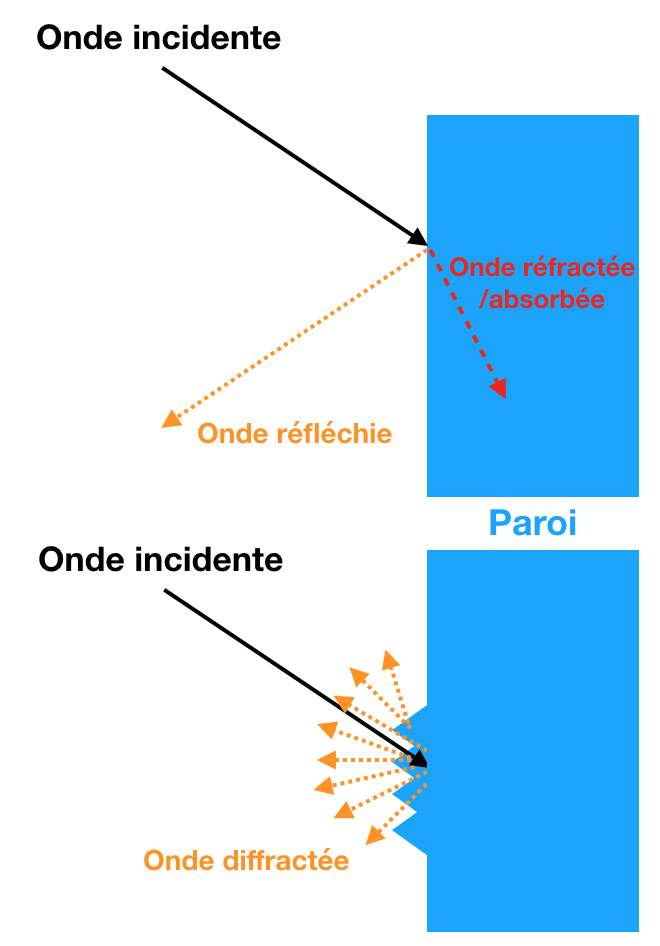
\includegraphics[width=0.5\linewidth]{images/schema_absorption}
	\caption[Les différents comportements d'une onde lorsqu'elle rencontre une paroi]{Les différents comportements d'une onde lorsqu'elle rencontre une paroi} %\footnotemark}
	\label{schema_absorption}
\end{figureth}
%\citefnt[Chap. 1]{aquaterra}

En se plaçant en un point à l'intérieur de la salle, on pourra alors recevoir un signal sonore comme étant la somme d'un champ direct et d’un champ réverbéré. Le son direct provient directement de la source sans avoir touché aucune surface. Le son réverbéré se distingue en deux catégories : les premières réflexions dont l'ensemble forment la texture du son et le champ diffus qui peut être assimilé à une somme infinie d'ondes se propageant dans toutes les directions \cite[p. 9]{jouhaneau}.
On comprend alors que les principaux facteurs qui vont influer sur l'acoustique perçue dans une salle sont : la source sonore, le milieu de propagation et la nature des parois et des obstacles.

\begin{figureth}
	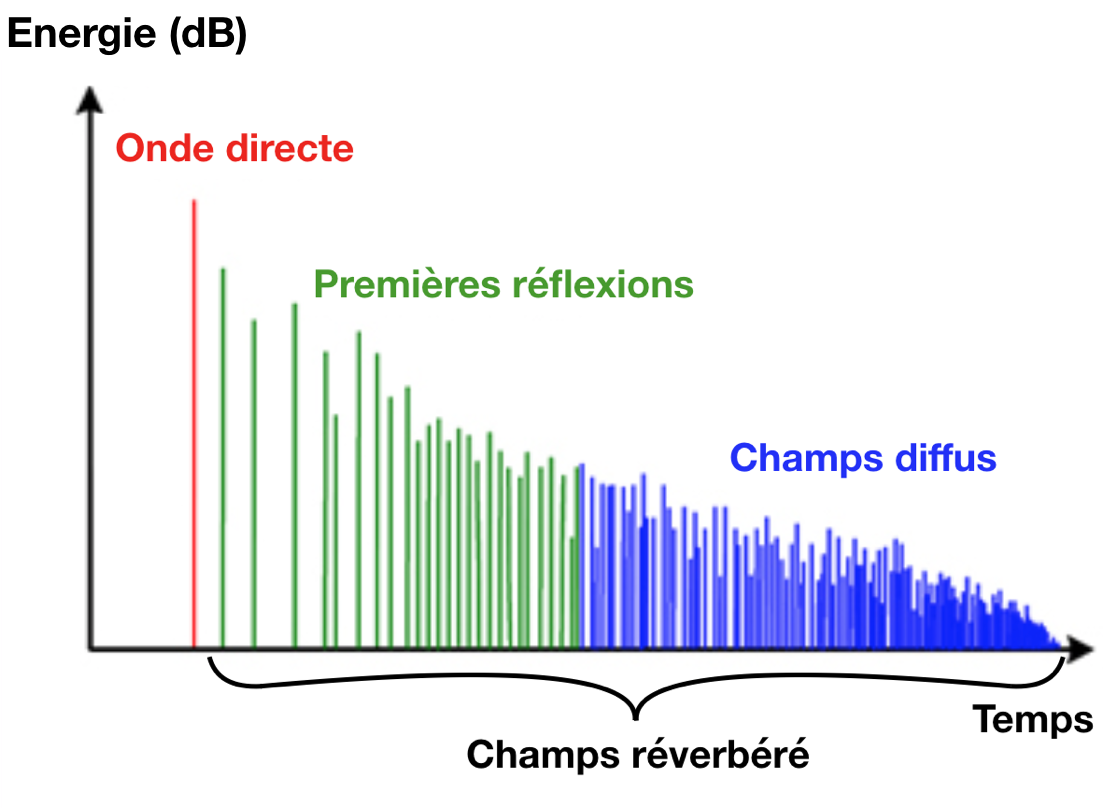
\includegraphics[width=0.7\linewidth]{images/RIR_schematique}
	\caption{Réponse temporelle d'une impulsion sonore dans une salle}
	\label{RIR_schematique}
\end{figureth}

La figure \ref{RIR_schematique}, illustrant la \gls{rir}, montre que l'information perçue est une succession d'ondes sonores arrivant décalées dans le temps. Si l'écart entre ces ondes est long, alors d'auditeur pourra les différencier et entendra le phénomène d'écho. Au contraire, si l'écart est suffisamment restreint et que les ondes sont mélangées au moment d'arriver à l'auditeur, alors celui-ci n'entendra qu'un son prolongé dont l'intensité diminue. Il s'agit de la réverbération \cite[p. 39]{sabine}. 





\subsection{Notion de flux d'intensité acoustique} \label{sect_intensite}
On définit par intensité acoustique la puissance transportée par les ondes sonores, par unité de surface, mesurée perpendiculairement à la direction de ce transfert \cite[IEC 60050]{cei}. Cette notion permet d'étudier le son perçu par les humains en la reliant à la pression acoustique qui va s'exercer de proche en proche dans l'air jusqu'à atteindre le tympan. Ainsi, la puissance sonore transportée par l'onde acoustique sera mesurable en un point de l'espace. Toute la puissance sonore mesurée en un point a une origine (actuelle ou passée) dans un flux d'énergie provenant d'une ou plusieurs directions identifiables. L'intensité acoustique mesure le flux résultant de ces transferts. 

L'intensité acoustique est un vecteur ayant pour origine le point de mesure et de même direction que le vecteur vitesse de l'onde. On peut l'écrire comme la moyenne dans le temps de l'intensité acoustique instantannée :
\begin{equation} 
\overrightarrow{I}(\overrightarrow{d},t) = \frac{1}{T} \int^T_0 p.\overrightarrow{v}dt,
\end{equation}
avec : 
\begin{itemize}
\item $p$ : la pression acoustique exprimée en $N.m^{-2}$ ou Pascal (Pa),
\item $\overrightarrow{v}$  : le vecteur vitesse.
\end{itemize}

Le \gls{spl} repère la valeur efficace de la pression acoustique par rapport à une valeur de référence, $20 \mu Pa$. On utilise, plutôt que le rapport brut, le décibel, qui représente dix fois son logarithme décimal. Ce repère a été choisi parce que, tout en étant simple et utilisant des nombres ronds, un décibel (une variation de 12 \%) représente à peu près la plus faible variation de pression acoustique que les humains puissent distinguer. Le niveau de référence, correspond de la même manière à la pression acoustique (dont l'intensité est de $1 pW/m^2$) au seuil de la perception humaine. On obtient ainsi un repère pratique où tous les niveaux sont des nombres positifs, et se passent de décimales. On a alors :

\begin{equation} 
L_p = 10 \log_{10}\left(\frac{p_{eff}^2}{p_{réf}^2}\right),
\end{equation}
avec :
\begin{itemize}
\item $L_p$ : le niveau de pression en dB,
\item $p_{eff}$ : la valeur efficace de pression \gls{RMS},
\item $p_{réf} = 20 \mu Pa$ : la référence de pression sonore.
\end{itemize}

Le flux de l'intensité acoustique instantanée à travers une surface  $\gamma(t)$ donnée correspond à l'énergie acoustique $E(t)$ transférée à travers cette surface, à l'instant considéré :

\begin{equation} 
E(t) = E_0 \int_{\gamma(t)} \overrightarrow{I(t)}.\overrightarrow{dS} \qquad \forall t > 0.
\end{equation}

L'acoustique suit le premier principe de la thermodynamique selon lequel il y a conservation d'énergie au cours du temps. Ainsi, pour une source sonore ponctuelle, si l'on néglige les effets de pertes liés à l'absorption du milieu de propagation, on a : 
\begin{equation} 
\int_{S(t)} \overrightarrow{I(t)}.\overrightarrow{dS} = 1 \qquad \forall t > 0.
\end{equation}

Après intégration sur la surface sphérique $S(t)$, nous pouvons écrire l'intensité acoustique infinitésimale telle que :
\begin{align} 
 \overrightarrow{I}(t) &= \frac{ \overrightarrow{d}(t)}{4\pi d(t)^3} \qquad \forall t > 0 \nonumber, \\
|| \overrightarrow{I}(t) || &= \frac{1}{4\pi d(t)^2} \qquad \forall t > 0,
\end{align}

\begin{figureth}
	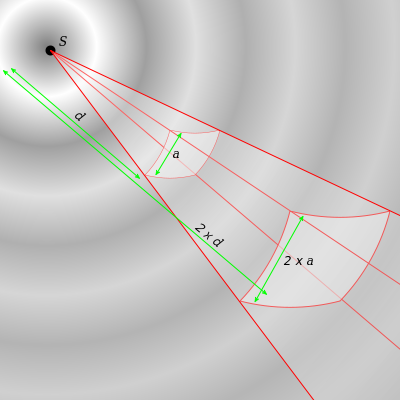
\includegraphics[width=0.5\linewidth]{images/flux}
	\caption{Représentation de la répartition du flux énergétique dans la propagation d'une onde sphérique}
	\label{flux}
\end{figureth}

On comprend que l'intensité décroit comme le carré de la distance et qu'une portion d'énergie considérée va donc être portée par un angle solide (voir fig. \ref{flux}). Ainsi, à une distance $d$ la même quantité d'énergie est répartie sur une surface de $a^2$ que à une distance de $2d$ sur une surface de $(2a)^2$. L'énergie se répartie donc sur une surface proportionnelle au carré de la distance. Sur une portion de $S(t)$ l'énergie est portée par un angle solide $\Omega_{S}$ tel que :

\begin{equation} \label{eq_energie}
E_{S}(t) = E_0 \int_{S(t)}  \frac{1}{4\pi  d(t)^2} dS = \frac{E_0}{4\pi}  \Omega_{S}.
\end{equation}

Cela traduit le fait que l'énergie d'un angle solide est constante au cours du temps et correspond à une portion de l'énergie initiale $E_0$.


%Par ailleurs, l'étude d'un signal sonore qui interagit avec un milieu ou un obstacle tel qu'un tympan par exemple se fait en pression ($N/m^2$ ou $Pa$). En conditions de champ libre, l'énergie acoustique est proportionnelle au carré de la pression acoustique :
%\begin{equation} 
%E_i \propto p^2
%\end{equation}



\subsection{Absorption atmostphérique}
 \label{sect_absAIr}
Pour se rapprocher d'un modèle réaliste de propagation d'onde, il est important de prendre en compte l'absorption atmosphérique. Ce phénomène est dû à la viscosité et la conduction thermique du milieu ainsi qu'à l'absorption des molécules. Ces effets vont provoquer une décroissance exponentielle de l'énergie d'onde \cite[p. 68-70]{jouhaneau}. Selon leur distance parcourue dans l'air, l'intensité acoustique va subir une atténuation en prenant en compte trois facteurs principaux : la température, l'humidité et le pression. La température et la pression atmosphérique de référence sont respectivement de 20°C et 101,325 kPa \footnote{International Standard Atmosphere}. Le coefficient d'atténuation dépend de la fréquence du son et peut être obtenue d'après les formules analytiques de la norme ISO-9613-1. Ces formules assez complexe ont été obtenue à l'aide de tables de mesures expérimentales.

% view-source:http://resource.npl.co.uk/acoustics/techguides/absorption/
Tout d'abord, nous calculons le facteur d'humidité $h$ correspondant à la concentration molaire de vapeur d'eau \cite[Annexe B, B.1]{iso} :

\begin{align*}
	C_h & = 4,6151 - 6,8346 \times \frac{273,15}{T}^{1,261},  \\
	h & = h_r \times 10^{\frac{C_h}{P_r}}, \\ 
\end{align*}
avec :
\begin{itemize}
\item $T$ : La température en Kelvin,
\item $P_r$ : La pression relative telle que $P_r = \frac{P_a}{101,325}$, avec $P_a$ la pression absolue,
\item $h_r$ : L'humidité relative mesurée en \%.
\end{itemize}
Nous exprimons ensuite les fréquences de relaxation de l'oxygène et de l'azote \cite[6.2, eq. 3 et 4]{iso}:

\begin{align*}
	fr_O & =  P_r \times \left(24 + \frac{40400 \times h \times (0,02 + h)}{0,391 + h}\right),  \\
	fr_A & =  \frac{P_r}{\sqrt{T_r}} \times \left(9 + 280 \times h \times \exp^{-4,17 \times (\frac{1}{\sqrt[3]{T_r}} - 1)}\right),
\end{align*}
avec :
\begin{itemize}
\item $T_r$ : La température relative à 20°C $\left(\frac{T}{293,15}\right)$,
\item $f$ : La fréquence en Hz.
\end{itemize}

Nous pouvons alors exprimer le coefficient d'absorption de l'air "$m$" (en dB/m) en fonction de la fréquence  \cite[6.2, eq. 5]{iso} :

\begin{equation*}
	m_{(dB/m)} = 8,686 \times f^2 \times \left(\frac{1,84 \times 10^{-11}}{P_r} \times \sqrt{T_r} + T_r^{\frac{-5}{2}} \times \left(0,01275 \times \frac{\exp{\frac{-2239,1}{T}}}{fr_O + \frac{f^2}{fr_O}} + 0,1068 \times  \frac{\exp{\frac{-3352}{T}}}{fr_A + \frac{f^2}{fr_A}}\right)\right).
\end{equation*}
On obtient le facteur final (en $m^{-1}$) par la formule :
\begin{equation}
	m = 10\log_{10}{\left(\frac{m_{(dB/m)}}{10}\right)} - 1.
\end{equation}

\begin{figureth}
	\begin{subfigureth}{0.8\linewidth}
		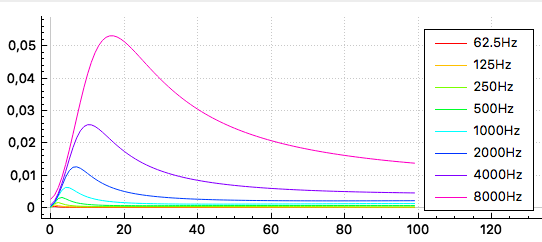
\includegraphics[width=\linewidth]{images/absorption}
		\caption{m(h) - Absorption de l'air en fonction de l'humidité relative (\%) pour différentes fréquences}
		\label{absorption}
	\end{subfigureth}
	\begin{subfigureth}{0.8\linewidth}
		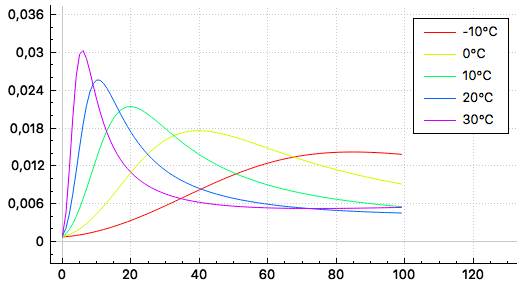
\includegraphics[width=\linewidth]{images/absorptionbis}
		\caption{m(h) - Absorption de l'air en fonction de l'humidité relative (\%) pour différentes températures}
		\label{absorptionbis}
	\end{subfigureth}
	\caption{Courbes d'absorption de l'air en fonction de l'humidité relative (\%) (ISO-9613) }
\end{figureth}

Notons tout de même que l'on aurait pu utiliser une formule simplifiée issue de la norme AFNOR S.30 009 qui donne des résultats similaires entre 20 et 80\% d'humidité relative \cite[p. 68-70]{jouhaneau} :
\begin{equation} \label{afnor}
	m = \frac{0,0275}{h} \times (\frac{f}{1000})^{1,7}.
\end{equation}
Néanmoins cette norme étant obsolète depuis 2016 et les résultats étant légèrement différents (voir fig. \ref{absorptionter}), nous optons pour la norme ISO-9613. \\

\begin{figureth}
	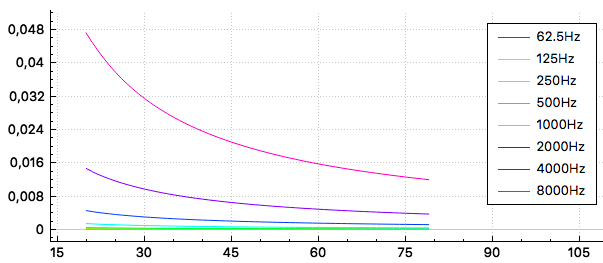
\includegraphics[width=0.8\linewidth]{images/absorptionter}
	\caption{m(h) - Courbes d'absorption de l'air en fonction de l'humidité relative (\%) pour différentes fréquences d'après l'équation \ref{afnor}}
	\label{absorptionter}
\end{figureth}

L'énergie de l'onde acoustique est ensuite déterminée par la formule suivante :
\begin{equation} \label{energie_absAir}
	E = E_0 e^{-m.d},
\end{equation}
avec :
\begin{itemize}
\item $E_0$ : l'énergie initiale,
\item $d$ : la distance parcourue par l'onde.
\end{itemize}
Cela permet donc de représenter l'absorption atmosphérique en fonction de la température et l'humidité pour différentes fréquences. On constate notamment que les basses fréquences sont très peu absorbées par l'atmosphère tandis qu'à partir de $2kHz$ l'absorption devient significative.



\section{Méthodes de calcul acoustique} 
Le calcul de l'acoustique d'une salle peut se faire selon différentes méthodes. Nous allons succinctement en présenter quelques unes afin d'en dégager les grands principes et les limites.

	\subsection{Principe statistique} \label{sect_sabine}

P. E. Sabine écrit en 1932 "\textit{Acoustics and architecture}" en reprenant les principes de son homonyme W. Sabine. Ce dernier décrivait 20 ans plus tôt des protocoles de test pour mesurer des temps de réverbérations dans les salles. P. E. Sabine considère que la réverbération suit un modèle purement statistique. De son point de vue, la densité d'échos à prendre en compte est suffisamment importante pour considérer le phénomène comme pseudo-aléatoire \cite[p. 19]{Kandelman}. Il suppose ainsi que l’énergie sonore et le temps de réverbération sont uniformes en tout point de la salle. Il exprime la notion de libre parcours moyen en ces termes : "\textit{Pour former l’image 2D des réflexions dans une salle, on peut imaginer une boule de billard lancée au hasard sur une table et noter la variation des longueurs des trajets entre deux impacts successifs. (…) La distance moyenne de ces longueurs peut être assimilée au libre parcours moyen d’une onde sonore dans la salle}" \cite[]{sabine2}. Ces considérations permettent d'exprimer le \gls{RT60} en fonction du volume de salle et de l'absorption des parois comme par exemple dans la formule dite "de Sabine" \cite[p. 71-81]{jouhaneau}: 

\begin{equation}
   	RT_{60} = \frac{k.V}{A},
\end{equation}
avec :
\begin{itemize}
\item $k \approx 0,163$,
\item $V$ : le volume de la salle,
\item $A$ : l'aire d'absorption équivalente telle que : 
\begin{equation}
   	A = \sum_{i=1}^N S_{i}\alpha_{i} + 4mV,
\end{equation}
\end{itemize}
où :
\begin{itemize}
\item $\alpha$ est le coefficient d'absorption de la i\up{e} paroi,
\item $m$ est l'amortissement du milieu (par exemple l'air),
\item $S_{i}$ est la surface de la i\up{e} paroi,
\item $N$ est le nombre de parois total.
\end{itemize}

Diminuer le volume sonore de $60dB$ garanti de passer en dessous au seuil audible (voir section \ref{sect_intensite}) c'est pourquoi cette limite est classiquement utilisée. La théorie de Sabine, est encore aujourd'hui couramment employée par les acousticiens des salles. Pourtant, cette hypothèse dite de "champ diffus" n’est plus vérifiée en pratique dès lors :
\begin{itemize}
\item la forme du milieu de propagation n’est plus homogène,
\item l’absorption acoustique devient importante,
\item l’absorption acoustique devient non uniforme,
\item la géométrie présente des ouvertures.
\end{itemize}
Pour remédier à cela, et notamment au critère sur l'absorption, Eyring propose avec le même modèle théorique une formule qui fournit de meilleurs résultats \cite[p. 217-241]{eyring}. Celle-ci, précisée dans les années 1920 et utilisée lors la conception acoustique de bâtiments durant leur phase de construction, est valable pour n'importe quel $\alpha$ :

\begin{equation}
   	RT_{60} = \frac{k.V}{4m.V - S\ln{(1-\alpha)}}.
\end{equation}
%
On constate que pour les faibles valeurs de $\alpha$, $\ln{(1-\alpha)} \simeq -\alpha$ et on retrouve la formule de Sabine.
 
	\subsection{Méthode de résolution exacte} \label{sect_resExacte}

La méthode de calcul exacte d'un champs sonore consiste à résoudre une équation aux dérivées partielles avec comme conditions aux limites, les parois de la pièce. Il s'agit ainsi de mailler le domaine d'étude par des petits éléments surfaciques (\gls{bem}), volumiques (\gls{fem}) ou sur une grille régulière (\gls{fdtd}). Sur chacun de ces éléments, on pourra calculer la pression acoustique $p(x,y,z,t)$ par résolution de l'équation d'onde de D'Alembert :
\begin{align} 
\Delta p-\frac{1}{c^2}\frac{\partial^2p}{\partial t^2} = 0, \ \ \ \footnotemark
\label{alembert}
\end{align}
\citefnt[p. 10]{Kandelman}
avec
\begin{itemize}
\item $\Delta$ : l'opérateur laplacien,
\item $c$ : la célérité de l'onde.
\end{itemize}
%
Pour cela, il faudra se placer dans les conditions de l'acoustique linéaire telles que \cite[p. 19]{jot}:
%
\begin{itemize}
\item l'air est un fluide parfait,
\item la température et la pression restent constantes,
\item la vitesse macroscopique du fluide est faible devant la célérité du son,
\item les fluctuations dues aux déplacements d'air sont faibles devant ces valeurs moyennes.
\end{itemize}
%
On pourra ensuite définir les impédances complexes des parois de la salle comme conditions aux limites (\gls{Dirichlet}, \gls{Neumann}, ...). \\

Les solutions de cette équation sur chacun des axes de l'espace (x, y, z) sont les $p_i$ tels que :
\begin{equation}
p_i(x_i,t) = f_+(t-\frac{x_i}{c}) + f_-(t+\frac{x_i}{c}),
\ \ \ \footnotemark
\end{equation}
\citefnt[p. 214-249]{alembert}
avec :
\begin{itemize}
\item $x_i$ : chacun des axes de l'espace (x, y, z),
\item $ f_+$ et  $f_-$ : des fonctions ne dépendant que d'une variable et définies à partir des conditions initiales. Elles représentent respectivement une onde se propageant sans se déformer vers $+\infty$ et $-\infty$.
\end{itemize}
Si l'on cherche à résoudre cette équation en tout point de l'espace et non seulement sur les axes cela devient beaucoup plus complexe.
L'équation d'Helmholtz apparait lorsque l'on cherche des solutions "stationnaires" de l'équation \ref{alembert} de D'Alembert telles que :
\begin{equation}
p(M) = u(M)e^{i\omega t},
\end{equation}
avec  $\omega = 2\pi f$ : la pulsation (rad/s). On a alors :

\begin{equation} \label{helmoltz}
(\Delta + k^2)u(M) = g(M)	 	\qquad  \forall M  \in \Omega,
\ \ \ \footnotemark
\end{equation}
\citefnt[eq. 2.1]{fem-bem}
avec :
\begin{itemize}
\item $g(M)$ : la distribution des sources,
\item $k$ : le nombre d'onde tel que $k = \frac{\omega}{c}$ avec $c$ la célérité du son,
\item $\Omega  \subset R^n$ : le domaine d'étude (voir fig \ref{schema_green}).
\end{itemize}
La fonction de Green qui s'écrit :
\begin{equation}
G(S,M) = -\frac{\exp^{ikr(S,M)}}{4\pi r(S,M)}
\ \ \ \footnotemark
\end{equation}
\citefnt[eq. 2.29]{fem-bem}
est une solution élémentaire pour la source ponctuelle $S$ de l'équation \ref{helmoltz} de Helmoltz telle que :
\begin{equation} \label{green}
(\Delta + k^2)G(S,M) = \delta_s(M)	 	\qquad  \forall M  \in \Omega,
\ \ \ \footnotemark
\end{equation}
\citefnt[eq. 2.2]{fem-bem}
avec : $\delta_s$ : la mesure de \gls{Dirac} centrée en S.

\begin{figureth}
	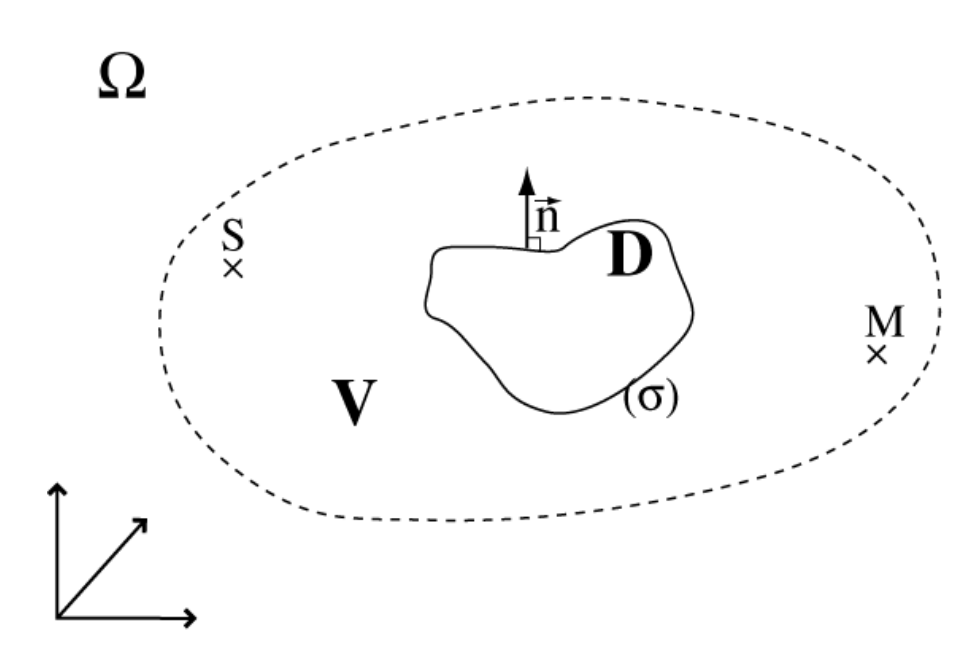
\includegraphics[width=0.6\linewidth]{images/green}
	\caption[Schéma général pour l'établissement de la représentation de Green]{Schéma général pour l'établissement de la représentation de Green \footnotemark}
	\label{schema_green}
\end{figureth}
\citefnt[fig. 2.1]{fem-bem}


%Alors en combinant les équations \ref{helmoltz} et \ref{green}, on obtient :
%\begin{equation}
%G(S,M)f(M)-p(M)\delta_s(M) = G(S,M)\Delta p(M)-p(M)\Delta G(S,M),	 	\qquad  \forall M  \in \Omega
%\ \ \ \footnotemark
%\end{equation}
%\citefnt[eq. 2.4]{fem-bem}
%
%En intégrant alors cette équation sur un volume V englobant le volume D et la source S, il s'ensuit :
%\begin{equation}
%\int_V G(S,M) f(M) dV - \int_Vp(M)\delta_s(M) dV = \int_V [G(S,M)\Delta p(M) - p(M)\Delta G(S,M)] dV,	 	\qquad  \forall M  \in \Omega
%\ \ \  \footnotemark
%\end{equation}
%\citefnt[eq. 2.5]{fem-bem}
%
%La  première  intégrale  dans  l'expression  ci-dessus  représente  le  champ  incident  c'est-à-dire  le  champ  rayonné  si  l'ensemble  de  sources  f(M)  était  seul  en  milieu  infini.  La deuxième  intégrale  est  le  champ  de  pression  en  un  point  M  de  l'espace  pour  une  source ponctuelle  S  (ce  facteur  serait  nul  si  la  source  S  n'était  pas  située  dans  le  volume  V).  Le membre  de  droite  peut  être  transformé  en  une  intégrale  de  surface  en  appliquant  le théorème  de  Green. Lorsque  l'on  fait  tendre  le  volume  V  vers  l'infini,  en  utilisant  la condition de Sommerfeld :
%\begin{equation}
%   \left \{
%	\begin{array}{r c l}
%		\underset{r \to \infty}{\lim} G &=& O(r^{(1-n)/2} \\
%		\underset{r \to \infty}{\lim} (\delta_r G - ikG) &=& O(r^{(1-n)/2} 
%	\end{array}
%   \right .
%   \footnotemark
%\end{equation}   
%\citefnt[eq. 2.3]{fem-bem}
Pour que le problème soit bien posé, il faut ajouter des conditions aux limites pour fixer le sens du temps et fermer le système \cite[p. 92]{BEM}. On introduit alors la condition de radiation de Sommerfield telle que :
\begin{equation}
r(\partial_ru' + iku') \to 0 \qquad r \to +\infty,
\end{equation}
avec $u' = u - \frac{u_i}{f}$, $u_i$ étant la pression incidente. On aboutit à une représentation intégrale sur la surface $\sigma$ du domaine D telle que :
\begin{equation}
u'(M) = p_0(M) - \int_\sigma G(S,M) \frac{\partial u'}{\partial_n}(M)dS -  \int_\sigma u'(M) \frac{\partial G}{\partial_n}(S,M) dS	 	\qquad  \forall M  \in \Omega.
\ \ \ \footnotemark
\end{equation}
\citefnt[eq. 2.6]{fem-bem}
%
Ainsi, si on connait $u$ et $\partial_n u $ la dérivée normale de u sur la surface $\sigma$, on peut calculer $u(M)$ en tout point M de $\Omega$. En acoustique des salles, il est cependant très difficile de calculer $u$ et $\partial_n u $.

%C'est à partir de cette équation que l'on pourra calculer la valeur de pression acoustique en tout point M de l'espace $\Omega$ non situé sur la frontière $\sigma$ du domaine D. Cette formule peut être généralisée pour donner l'équation intégrale de Helmottz-Kirchhoff :
%
%\begin{equation}
%c(M)p(M) = p_0(M) + \int_\sigma [p(M) \frac{\partial G}{\partial n_S}(S,M) - G(S,M) \frac{\partial p}{\partial n_S}(M)] dS,	 	\qquad  \forall M  \in \Omega
%\ \ \ \footnotemark
%\end{equation}
%\citefnt[eq. 2.7]{fem-bem} 
%
%Avec : \\
%\begin{equation}
%c(M) = 1 - \frac{1}{4\pi} \int_\sigma \frac{\partial}{\partial n} (\frac{1}{r})dS
%\ \ \ \footnotemark
%\end{equation}
%\citefnt[eq. 2.8]{fem-bem} 







	\subsection{Méthodes géométriques}
	
Les méthodes géométriques sont largement utilisées dans le domaine de l'acoustique de salle. Elles se basent sur le trajet que parcourt l'onde sonore entre une source et un récepteur (fig. \ref{geometrique}). L'onde, percutant les parois, subit un changement de direction de propagation. Par ailleurs, chaque paroi ou obstacle porte une \gls{impedance} lié à la nature de son matériau qui atténuera l'énergie de l'onde réfléchie en fonction de sa fréquence.

\begin{figureth}
	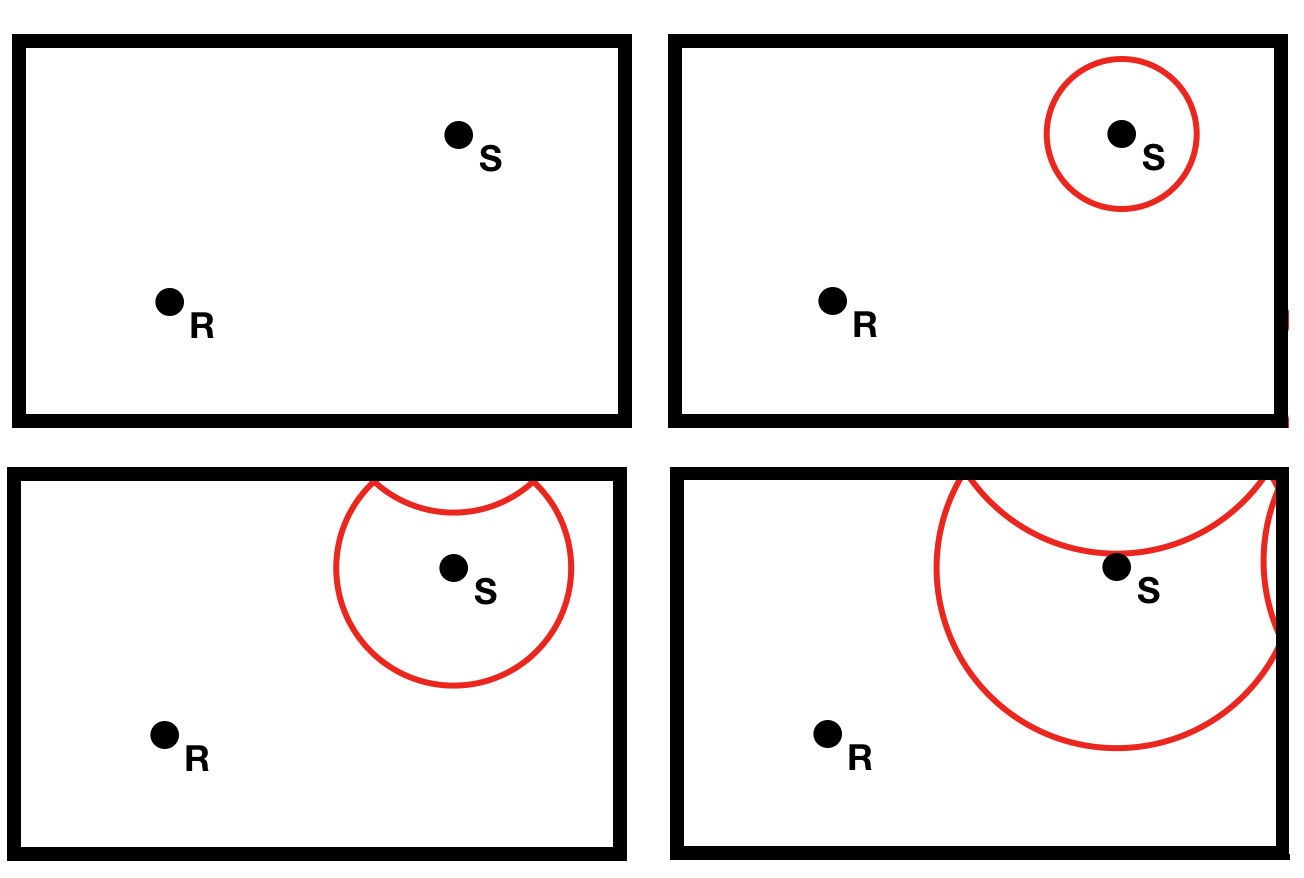
\includegraphics[width=0.8\linewidth]{images/geometrique}
	\caption{Vu 2D de la propagation d'une onde sphérique dans une salle rectangulaire}
	\label{geometrique}
\end{figureth}

En pratique certaines méthodes de calcul permettent de simuler ce comportement. Tout d'abord, la méthode dite de lancé de rayon (\textit{ray-tracing})\cite[p.449-468]{raytracing} qui est très souvent utilisée dans les logiciels d'acoustique de salle (Odéon \cite[page web]{odeon}, CATT-acoustic \cite[page web]{catt}, ...). Cette approche suppose que l’énergie sonore émise depuis une source est repartie sur un certain nombre de rayons rectilignes déviés de manière \gls{speculaire} lors de leur rencontre avec les parois. La mesure d'énergie est alors réalisée par comptage du nombre de rayons qui traversent une sphère transparente. La précision de mesure sera ainsi fonction du nombre de rayons émis et de la taille de la sphère-récepteur. Il peut notamment y avoir beaucoup de perte d'information si le domaine de propagation est complexe \cite[p. 60]{picaut}. Il s'agit donc d'une méthode très puissante pour simuler les réflexions géométriques sur les parois mais inadaptée pour simuler les effets de diffraction. Effectivement, pour simuler ces effets il faudrait re-générer un panel de rayons pour chaque réflexion sur une paroi diffractante, ce qui augmenterait exponentiellement le nombre de rayons et donc le temps de calcul. Pour résoudre ce problème, une approche de type "lancer de particules" sert d'alternative au lancer de rayon. Dans ce concept très similaire, lors du contact avec une paroi, la particule sera réfléchie de manière statistique. Par exemple, si $\alpha$ est le coefficient d'absorption de la paroi, alors, la particule aura une probabilité de $(1-\alpha)$ d'être réfléchie et une probabilité $\alpha$ d'être absorbée. En ce sens, il est également possible de déterminer, selon une loi de probabilité, l'angle de réflexion et simuler ainsi une "pseudo-diffusion" des matériaux \cite[p. 62]{picaut}. Néanmoins, dans certains contextes il est possible de négliger les effets de diffraction.


Il existe aussi la méthode dite des "sources-images" \cite[p.6]{jouhaneau} très appréciée pour son approche spatialisée des réflexions sonores. Cette méthode est fondée sur la construction de sources virtuelles, images de la source réelle, construite par symétrie par rapport aux parois de l'enceinte. La contribution énergétique de chaque source-image est celle habituellement rencontrée dans le cas de la propagation en champ libre, pondérée par le coefficient d’absorption des parois considérées \cite[p. 60]{picaut}.
Le problème de cette méthode est que l'on génère l'ensemble des sources-images d'une salle et qu'il est ensuite difficile de discriminer celles qui sont perçues et celles qui sont bloquées par des obstacles. Cela est donc plutôt adapté aux pièces de forme concave et vide. Par ailleurs, comme pour le tracé de rayons, les effets de diffraction ne sont pas pris en compte. 


\begin{figureth}
	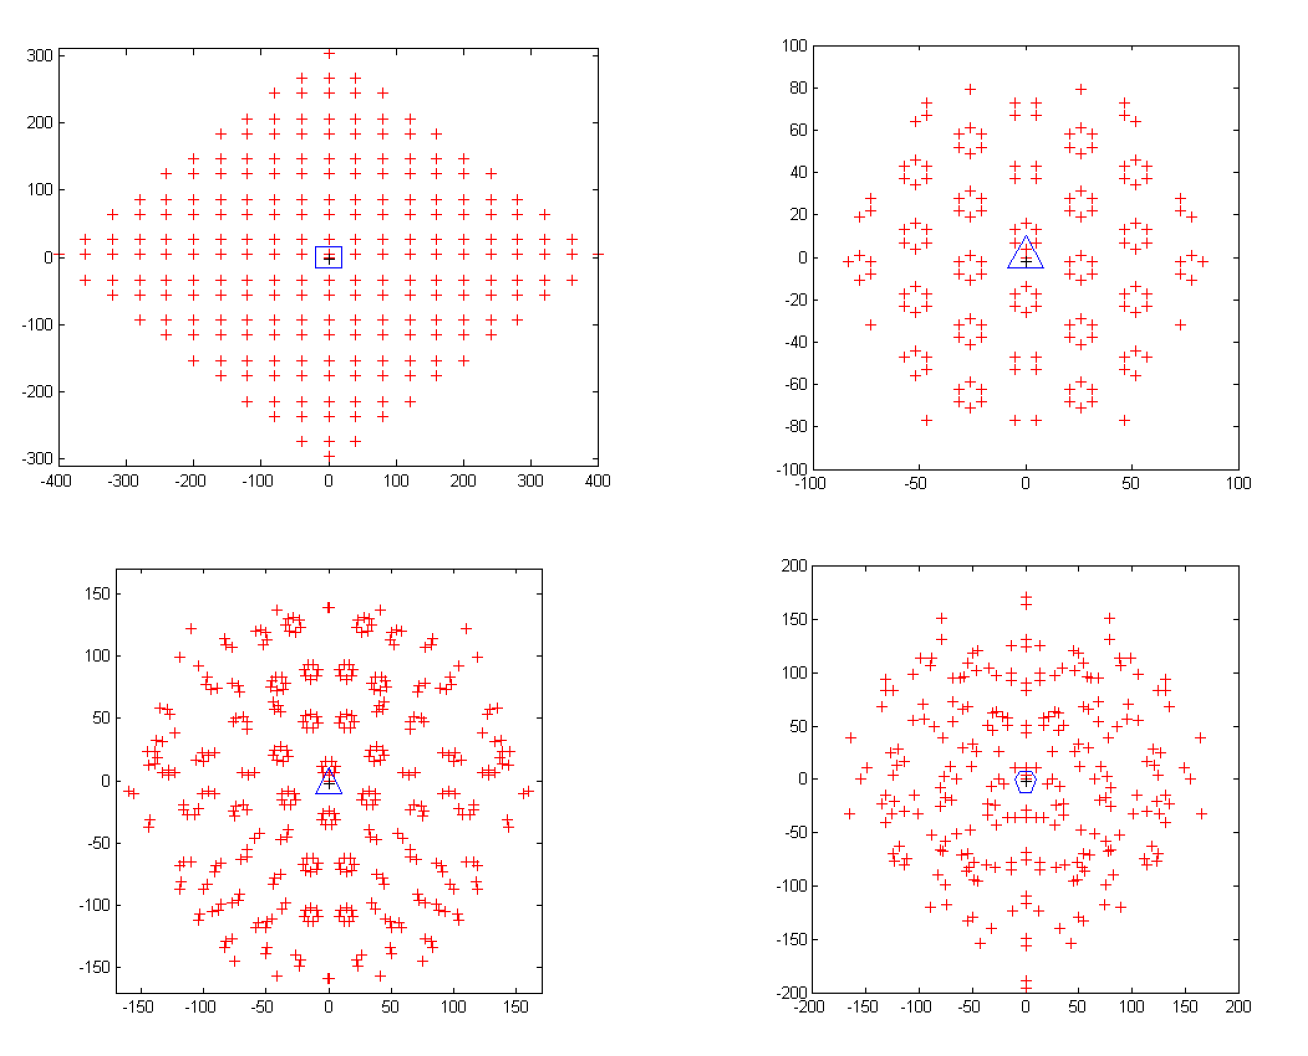
\includegraphics[width=\linewidth]{images/constellations}
	\caption[Différentes constellations de salle : la densité de sources reste constante]{Différentes constellations de salle : la densité de sources reste constante \footnotemark}
	\label{constellations}
\end{figureth}
\citefnt[Fig. 61]{Kandelman}

%C'est sur ce type d'approche géométrique que le choix s'est porté dans le cadre du projet. Nous allons donc détailler dans le prochain chapitre comment coupler ces concepts géométriques afin de répondre à la problématique. 

		
		
		
		
		
		
		
		
		
		
		
		
		
\chapter{Développement d'une méthode couplée}
	\citationChap{
	Quand on aime on ne compte pas... \\
	Ça tombe bien, je suis mauvaise en calcul !
	}{Sophie Lesellier}
	\minitoc
	\newpage
	
\section*{Introduction} \label{sect_methodecouplee}
Le projet a pour essence le calcul de l'acoustique du théâtre d'Orange. Cela soulève certaines problématiques qui nous ont poussé à développer une méthode de calcul hybride. Effectivement, ce cas d'application impose le cahier des charges suivant :
\begin{itemize}
	\item Pouvoir traiter une salle de grande dimension,
	\item Pouvoir traiter un volume ouvert,
	\item Prendre en compte l'absorption atmosphérique,
	\item Calculer les résultats sur une large plage de fréquences audibles par l'être humain (50-15000Hz),
	\item Permettre l'étude du déplacement de l'onde sonore dans l'espace.
\end{itemize}
Par ailleurs, il faut pouvoir s'interfacer au modèle numérique réalisé sous Blender et décrit dans la partie \ref{part_1}. Pour cela, nous devons rajouter les caractéristiques suivantes au cahier des charges :

\begin{itemize}
	\item Utiliser un maillage surfacique sans contrainte sur la dimension ou le raffinement des faces.
	\item Pouvoir traiter plusieurs centaines de milliers de faces en un temps relativement court.
	\item Pouvoir modifier facilement les coefficients d'absorption des matériaux.
\end{itemize}

Ces contraintes sont nécessaires afin de rendre l'étude acoustique du théâtre d'Orange (ou de tout type de monument similaire) accessible à des utilisateurs de Blender. Ainsi, la géométrie où la nature des matériaux pourra être facilement modifiable et une large série de tests comparatifs peut être menée rapidement. Le but étant de pouvoir tester des hypothèses de restitution sans avoir à multiplier les manipulations entre chaque calcul.

%Afin de répondre à ces contraintes, nous avons opté pour certains choix technologiques. Premièrement, le code est développé en C++ pour des raisons de rapidité de calcul. Il s'agit d'un exécutable "client" paramètrable directement depuis l'interface Blender. Au lancement du programme, Blender exporte le maillage dans un fichier qui sera traité par le logiciel "client". Ainsi, l'outil acoustique est transparent pour l'utilisateur et l'accès au maillage est donc immédiat. Le format de fichier s'est porté sur le \gls{obj}. Celui-ci est un des formats les plus courants et il est disponible sur la plupart des logiciels de \gls{cao}. Ainsi, l'outil n'est pas exclusif et pourra travailler à partir de n'importe quel maillage au format \gls{obj}.

Sachant cela, nous avons dans un premier temps tenté de réaliser des analyses par méthode de résolution exacte (voir section \ref{sect_resExacte}) mais nous avons vite compris que la géométrie de la salle rendrait la résolution très difficile. Effectivement, le nombre d'éléments que doit comporter le maillage est dépendant de la longueur d'onde \cite[p. 740]{beamtracing}. Dans un cas comme le théâtre d'Orange où les longueurs se comptent en dizaines de mètres et les fréquences en kilo-Hertz (fréquences audibles), il faut raffiner les mailles à l'échelle du millimètre, ce qui génère des milliards d'éléments. Ce genre de problème est aujourd'hui particulièrement complexe à mettre en place de part la puissance de calcul et l'espace mémoire nécessaire. Par ailleurs la création d'un maillage de type conforme, c'est à dire avec des triangles de taille régulière et dont les angles ne sont pas trop aigües, représente une difficulté à part entière.
Au début du projet, nous avions tenté d'analyser une version très simplifiée du théâtre à des fréquences très faibles. Nous voulions notamment tester l'impact de la forme incurvée des gradins en comparant de manière relative différents maillages. Le raffinement fut effectué à l'aide de l'outil "\textit{mmg}" \cite[github]{mmg} développé en partie à l'\gls{iscd}. Les calculs acoustiques ont été fait avec l'outil "\textit{Gypsilab}" \cite[github]{gypsilab} développé par le \gls{cmap}. En conservant à peu près des dimensions du théâtre et pour de faibles fréquences, nous obtenions déjà plusieurs centaines de milliers d'éléments et des temps de calcul de quelques dizaines de minutes (sur un ordinateur standard). En augmentant la fréquence et donc le raffinement du maillage nous aurions rapidement atteint les limites des machines en terme de mémoire avec des temps de calcul considérables. Or cela ne coïncidait pas du tout avec les objectifs établis. Le constat a alors été que ce type d'étude n'était pas adaptée au cahier des charges.

\begin{figureth}
	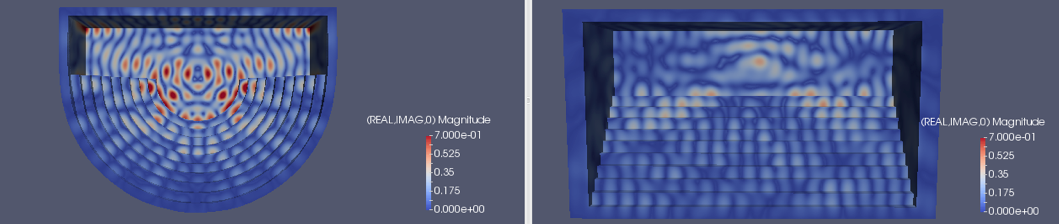
\includegraphics[width=\linewidth]{images/BEM}
	\caption{Comparaison d'un théâtre simplifié avec gradins coniques ou gradins cubiques par méthode des éléments finis de frontière à 50Hz}
	\label{BEM}
\end{figureth}

La meilleure option fut alors de se tourner vers des solutions approchées utilisant des méthodes de calcul de type géométrique. Cela est acceptable en se plaçant dans l'approximation dite "hautes fréquences" soit typiquement lorsque $kv >> 1$ ($k$ étant le nombre d'onde et $v$ le volume de la salle). La méthode développée, dite "couplée", consiste à propager des rayons à partir d'une source et, à chaque réflexion sur les parois, d'analyser ceux qui traversent une sphère-récepteur pour créer des sources-images. Grâce au temps de parcours des rayons et d'après les hypothèses statistiques de Sabine (voir section \ref{sect_sabine}), il est alors possible de créer la \gls{rir}. Celle-ci pourra alors être convoluée à un signal audio afin de pouvoir écouter le son réverbéré (voir section \ref{sect_TDS}).

Le chemin de chacun des rayons permet de situer dans l'espace les sources-images correspondantes, c'est à dire les images de la source suite aux divers réflexions sur les parois. Nous obtenons ainsi une constellation de sources-images portant des énergies atténuées par l'absorption des parois. Cela permettra par la suite de spatialiser le son, c'est à dire de savoir d'où proviennent les différents échos. Il est alors possible d'écouter le son réverbéré en trois dimensions. 

Ce chapitre vise à détailler ce processus. Notons néanmoins que les effets de diffraction ne seront pas traités même si, comme nous l'avons évoqué précédemment au sujet du lancer de particules, il est possible d'utiliser des lois de probabilité pour répartir les rayons réfléchis selon différentes directions \cite[p.187-199]{diffusion}. Nous choisissons néanmoins de ne fonctionner qu'avec des réflexions spéculaires car le sujet de la diffraction est extrêmement vaste et complexe. Il s'agit d'un sujet à part entière que l'on ne traitera pas durant ce projet de thèse mais qui pourra venir l'enrichir par la suite. Les grandes dimensions du théâtre d'Orange et la gamme de fréquence utilisée permettent de se placer dans l'approximation "hautes fréquences".

\section{Notion d'onde sphérique discrétisée} \label{sect_discretise}

\begin{figureth}
\begin{subfigureth}{0.55\textwidth}
	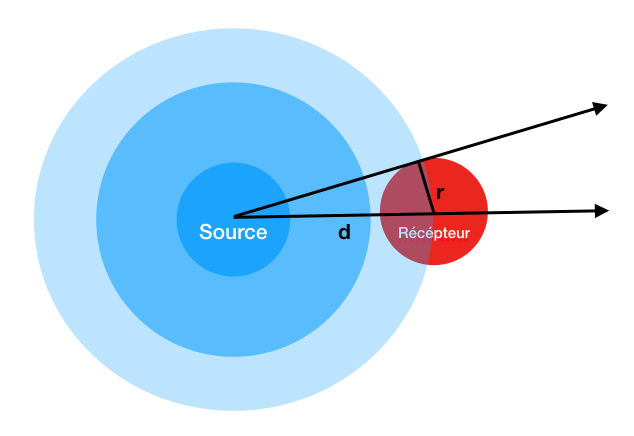
\includegraphics[width=\linewidth]{images/schema_propagation}
	\caption{Schéma en deux dimensions d'une onde sphérique dont une portion d'énergie est mesuré par un récepteur de rayon r.}
	\label{schema_propagation}
\end{subfigureth}
\qquad
\begin{subfigureth}{0.35\textwidth}
	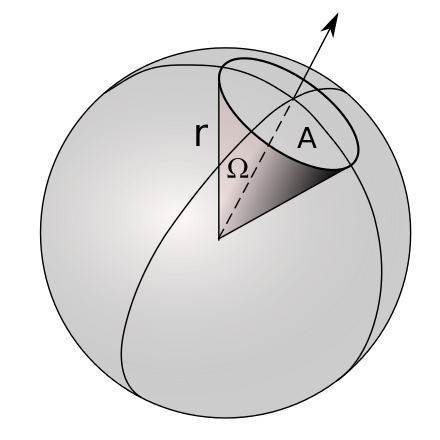
\includegraphics[width=\linewidth]{images/angle_solide}
	\caption{Représentation de l'angle solide d'un cône de révolution \footnotemark}
	\label{angle_solide}
	\end{subfigureth}
	\caption{Représentations du principe de mesure de l'angle solide}

\end{figureth}
\citefnt[image]{angle_solide}


Dans ce développement, nous choisissons d'utiliser des sources omnidirectionelles, c'est à dire qui propagent le son de manière uniforme dans toutes les directions de l'espace. Néanmoins, notons qu'il serait possible d'utiliser d'autres types de source en changeant la répartition des rayons émis. Ces sources sont de type impulsionnelles. Effectivement, un signal sonore continu peut-être discretisé par une suite d'impulsions (c'est d'ailleurs le cas de tout signal numérique qui est échantillonné à une certaine fréquence). Une impulsion étant un signal d'un temps infiniment court, l'énergie émise depuis la source sera répartie sur la surface d'une sphère en expansion comme nous l'avons vu dans la section \ref{sect_intensite} (voir fig. \ref{schema_propagation}). Seul le flux passant par le récepteur sera capté. Ainsi, l'énergie perçue est l'intersection entre la sphère d'émission et la sphère de réception. Il s'agit donc d'un angle solide $\Omega$ de type conique (voir fig. \ref{angle_solide}) tel que :

\begin{equation}
\Omega =\frac{S}{d^2},
\end{equation}
avec  :
\begin{itemize}
\item $\Omega$ : l'angle solide en stéradian (sr),
\item $S$ : l'aire de la portion de sphère d'émission interceptée en mètre carré ($m^2$),
\item $d$ : le rayon de la sphère d'émission en mètre (m).
\end{itemize}


Par ailleurs, pour simplifier les calculs, la propagation de l'onde peut être discretisée en $N$ rayons émis depuis la source de manière uniforme. Chaque rayon porte l'énergie $E_i$ tel que :

\begin{equation}
E(t) = \sum_{i=1}^N E_i(t) = \frac{E_0}{4\pi}  \sum_{i=1}^N \Omega_i  \qquad \forall t > 0,
\end{equation}
avec  $\Omega_i$ : l'angle solide élémentaire tel que $ \sum_{i=1}^N \Omega_i = 4\pi$. \\



 Le problème de cette approximation est qu'elle apporte de l'erreur au résultat. Effectivement, l'information n'est plus portée par un cône mais par des rayons. Toute mesure prise entre deux rayons sera donc impossible. Il faut alors limiter au maximum cette erreur et réduire l'écart entre deux rayons. On pourra ainsi considérer qu'une grande quantité de rayons peut être assimilée à un cône plein. Pour cela, on souhaite connaitre la distance au bout de laquelle les rayons sont suffisamment séparés les uns des autres pour être distingués. En se plaçant dans le cas théorique d'une source et d'un récepteur en espace libre, il faut alors exprimer le temps au bout duquel il est possible de capter moins d'un rayon dans la sphère de mesure. 
%
\begin{figureth}
	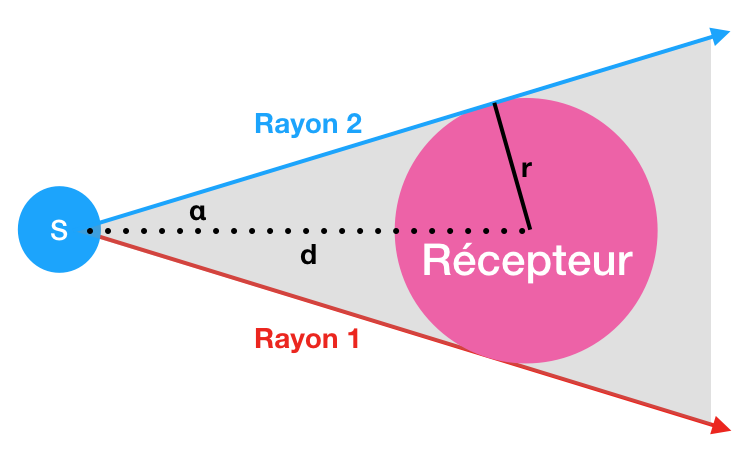
\includegraphics[width=0.7\linewidth]{images/schema_rayon}
	\caption{Schéma d'un récepteur captant au moins un rayon.}
	\label{schema_rayon}
\end{figureth}
%
Pour se faire, nous utilisons la formule de l'angle solide d'un cône de révolution \cite[Angle solide d'un cône de révolution]{cone} de demi-angle au sommet $\alpha$ (voir fig. \ref{angle_solide}) :
\begin{equation}
	\Omega_i = 2\pi(1-cos(\alpha)).
\end{equation}
%
Or, cet angle solide peut aussi s'exprimer par :
\begin{equation}
	\Omega_i = \frac{4\pi}{N}.
\end{equation}
%
Ainsi, on obtient d'après Pythagore (voir fig. \ref{schema_rayon}) :
\begin{align}
	cos(\alpha) & =  \frac{\sqrt{d^2-r^2}}{d}, \nonumber \\
	& =  \sqrt{1-\frac{r^2}{d^2}},
	%& \simeq 1-\frac{1}{2}\frac{r^2}{d^2}
\end{align}
avec  :
\begin{itemize}
\item $r$ : le rayon du récepteur,
\item $d$ : la distance maximale du récepteur à la source,
\item $N$ : le nombre de rayons total.
\end{itemize}
%
En normalisant l'énergie ($E_0 = 1$), on obtient alors :

\begin{align} 
	2\pi \left(1-\sqrt{1-\frac{r^2}{d^2}} \right) &= \frac{4\pi}{N} \nonumber,\\	
	\sqrt{1-\frac{r^2}{d^2}} &= 1-\frac{2}{N} \nonumber,\\
	1-\frac{r^2}{d^2} &= \left(1-\frac{2}{N}\right)^2 \nonumber,\\
	\frac{r^2}{d^2} &= \frac{4}{N^2}(N-1) \nonumber,\\
	 \frac{r}{d} &=  \frac{2}{N} \sqrt{N-1}. \label{seuil_arret}
\end{align}
%
Nous constatons qu'en fixant $N$ (le nombre de rayons total émis depuis la source) et $r$ (le rayon de la sphère de mesure), nous pouvons connaitre la distance $d$ au bout de laquelle la probabilité de ne capter aucun rayon ne sera plus nulle. En pratique, on voudra réduire encore l'erreur et il faudra arrêter la mesure avant d'arriver à cet extreme. On pourra alors fixer un nombre $n$ de rayons minimum à capter. Par exemple si on fixe $n$ à 100 rayons, on s'assure que la mesure comprend au moins 100 portions de la sphère énergie et on revient statistiquement à un modèle quasi-continu.


Pour établir la nouvelle expression, il suffit de refaire les mêmes calculs en considérant que :
\begin{equation}
	\Omega_i = n.\frac{4\pi}{N}. \\
\end{equation}
%
L'équation \ref{seuil_arret} s'écrit donc :
\begin{align} 
	\frac{r}{d} =  \frac{2n}{N} \sqrt{\frac{N}{n}-1} % \\
 	\quad \Rightarrow  \quad %\\
	 d_{max} =  \frac{N.r}{2n\sqrt{\frac{N}{n}-1}}.
\end{align}
%
Aussi, si $N >> n$ l'expression se simplifie par : 
\begin{align} \label{eq_dmax}
	 d_{max} \approx  \frac{r}{2} \sqrt{\frac{N}{n}}.
\end{align}

Nous limitons de cette façon le calcul aux premières réflexions de la réponse impulsionnelle. Cependant, les \gls{rir} sont en général calculées jusqu'à ce que l'énergie diminue de $60dB$. Il s'agit d'un critère d'arrêt classique car, comme expliqué dans la section \ref{sect_sabine} il assure de couvrir la plage d'audition humaine. Or avec notre méthode, nous ne prenons plus de mesure à partir d'un certain temps, correspondant à la distance $d_{max}$. Il faudra alors jouer sur les paramètres $N$, $r$ ou $n$ pour s'assurer de dépasser le \gls{RT60}. En pratique, le temps de calcul sera très sensible à la valeur de $N$ tandis que la précision dépendra de $r$ et $n$. Ainsi, une possibilité est d'arrêter la mesure lorsque $d_{max}$ est atteinte et de compléter le champs diffus de manière statistique. Cela est envisageable d'après les hypothèses de Sabine qui supposent que le champs diffus devient pseudo-alétoire. La réponse impulsionnelle obtenue par tracé de rayons peut ainsi être prolongée par régression linéaire pour atteindre \gls{RT60}. \\




%\begin{figureth}
%	\begin{subfigureth}{0.45\textwidth}
%		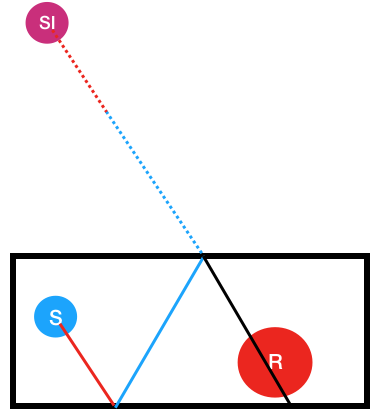
\includegraphics[width=0.9\linewidth]{images/schema_SI}
%		\caption{Schéma de la création d'une source image par réflexions successives d'un rayon sur les parois d'une salle}
%		\label{schema_SI}
%	\end{subfigureth}
%	\qquad
%	\begin{subfigureth}{0.45\textwidth}
%		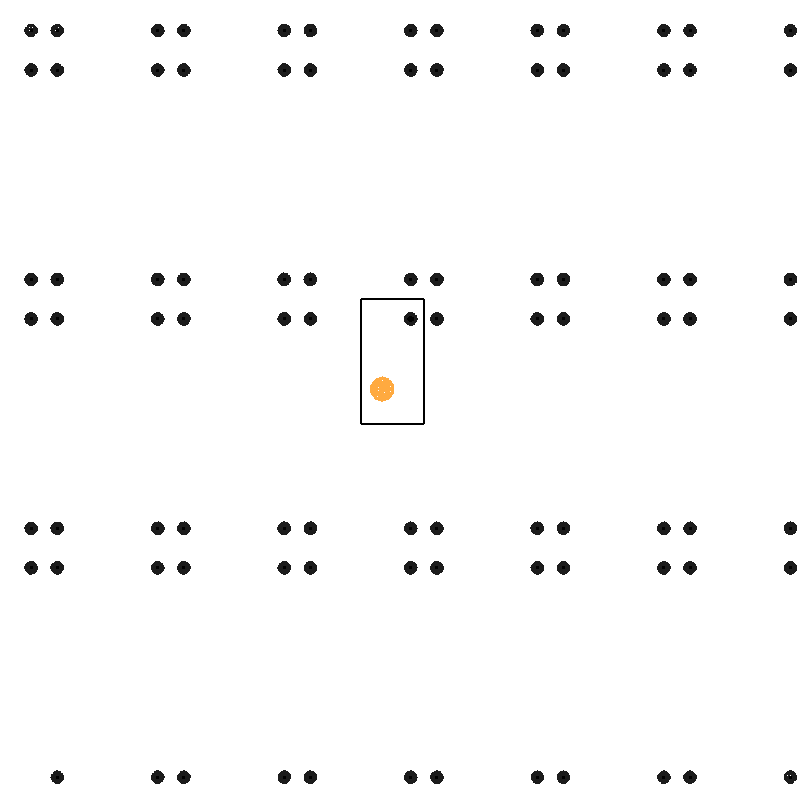
\includegraphics[width=\linewidth]{images/constellation}
%		\caption{Constellation de sources-images dans une salle rectangulaire}
%		\label{constellation}
%	\end{subfigureth}
%	\caption{Représentations du principe de sources-images}
%\end{figureth}










\section{Environnement géométrique}

\subsection{Maillage de salle et matériaux} \label{sect_lectMat}
%L'une des premières étape consiste à lire une base de données (issue du logiciel Odéon) pour récupérer les coefficients d'absorption des différents matériaux disponibles. Chaque matériau possède un numéro-référence qui devra être stipulé dans le nom du matériau sous Blender. Ces numéros sont associés dans la base de données à huit coefficients d'absorption correspondant aux bandes d'octave : 62,5Hz, 125Hz, 250Hz, 500Hz, 1kHz, 2kHz, 4kHz, 8kHz. Ces huit bandes de fréquence permettent de couvrir une large plage des fréquences audibles par l'être humain. Il existe de nombreuses bases de données recensant ces coefficients d'absorption pour tout type de matériaux. Elles sont en générales créées de manière expérimentale et celle que nous utilisons a l'avantage d'être très complète et en libre accès sur le site d'Odéon \cite[Materials]{odeon}

Comme nous l'avons vu précédemment, nous allons travailler à partir d'un maillage existant, qui sera dans notre cas d'application le théâtre d'Orange (voir partie \ref{part_1}) mais qui pourrait être n'importe quel maillage de salle. La méthode se doit donc d'être générique. Cependant notons qu'il sera obligatoire d'avoir des faces triangulaires et que les normales devront être orientées vers l'intérieur de la salle (voir fig. \ref{normales}).

\begin{figureth}
	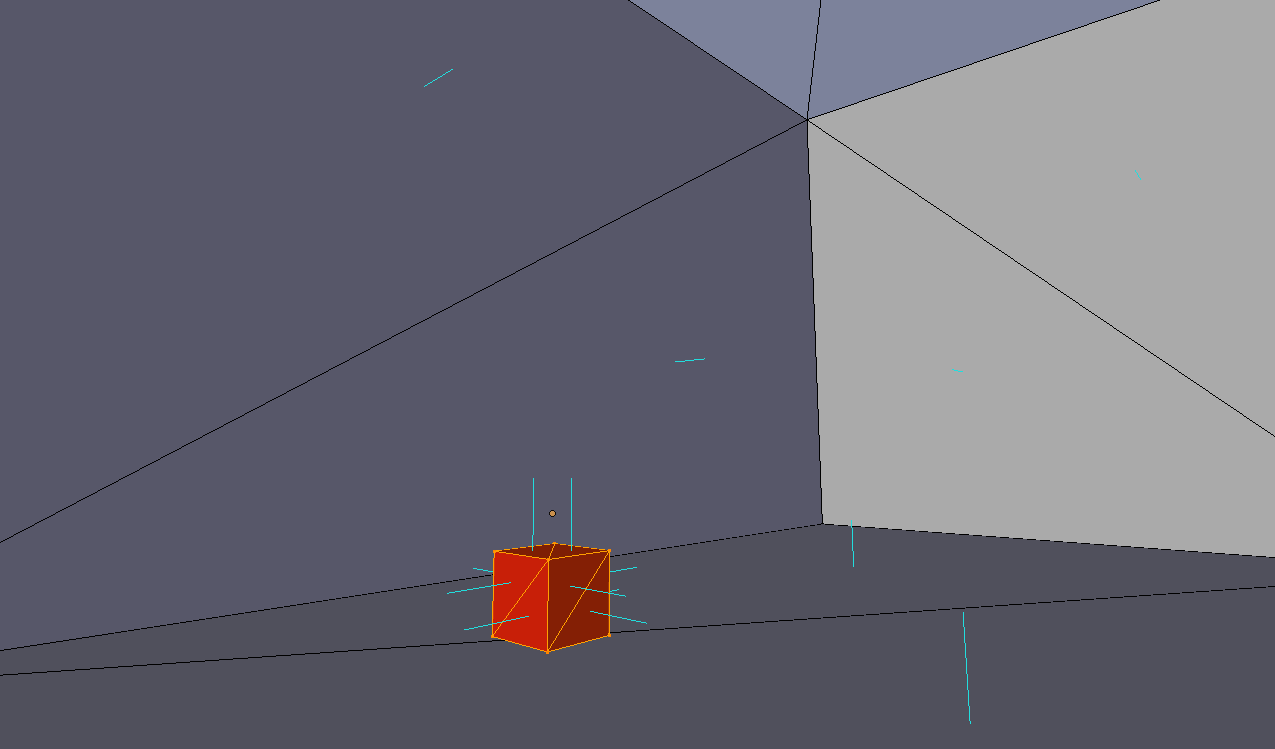
\includegraphics[width=0.8\linewidth]{images/normales}
	\caption{Représentation d'un maillages surfacique à faces triangulaires composé d'une salle et d'un obstacle et dont les normales (en bleu) sont orientées vers l'intérieur de la salle.}
	\label{normales}
\end{figureth}

Chaque face triangulaire est donc considérée comme une paroi à laquelle il faut affecter un matériau. A un matériau on associe huit coefficients d'absorption correspondant aux bandes d'octave : 62,5Hz, 125Hz, 250Hz, 500Hz, 1kHz, 2kHz, 4kHz, 8kHz. Ces huit bandes permettent de couvrir une large plage des fréquences audibles par l'être humain. L'absorption de l'onde sonore dépendra donc de la fréquence et il faudra calculer huit réponses impulsionnelles. Il existe de nombreuses bases de données recensant ces coefficients d'absorption pour tout type de matériaux. Elles sont en générales créées de manière expérimentale dans un local spécialement aménagé. L'erreur est de l'ordre de 15\% \cite[]{acouphile}. La base que nous utilisons a l'avantage d'être très complète et en libre accès sur le site d'Odéon \cite[Materials]{odeon}. Les coefficients sont sans unité et correspondent à un ratio d'absorption compris entre 0 et 1. Le tableau \ref{tab_coeff_abs} présente quelques exemples de coefficients d'absorption. L'énergie d'un rayon ayant été réfléchi par plusieurs parois sera proportionnelle à :
\begin{equation} \label{eq_coeff_abs}
E = \prod_{i=0}^n (1-\alpha_i),
\end{equation}
avec: 
\begin{itemize}
\item $n$ : le nombre de parois rencontrées,
\item $\alpha_i$ : le coefficient d'absorption de la i-ème paroi.
\end{itemize}
%
\begin{tableth} \label{tab_coeff_abs}
\footnotesize
	\begin{tabular}{| c | m{2.5cm} | *{8}{c|}}
		\hline
		Référence & Nom du matériau & 62,5Hz & 125Hz & 250Hz & 500Hz & 1kHz & 2kHz & 4kHz & 8kHz \\
		  \hline
		  \hline
		   1 & 100\% absorbent & 1 & 1 & 1 & 1 & 1 & 1 & 1 & 1 \\
		   \hline
		2 & 100\%reflecting & 0 & 0 & 0 & 0 & 0 & 0 & 0 & 0 \\
		   \hline
		107 & Concrete block, coarse\footnotemark & 0.36 & 0.36 & 0.44 & 0.31 & 0.29 & 0.39 & 0.25 & 0.25 \\
		   \hline
		3000 & Hollow wooden podium\footnotemark & 0.4 & 0.4 & 0.3 & 0.2 & 0.17 & 0.15 & 0.1 & 0.1 \\
	     \hline
	 \end{tabular}
	\caption{Exemples de coefficients d'absorption de la base de données Odéon}
\end{tableth}
\addtocounter{footnote}{-1}
\footnotetext{Harris, 1991}
\addtocounter{footnote}{1}
\footnotetext{Dalenbäck, CATT}
%



Notons par ailleurs que l'on défini la ou les sources sonores par une position ponctuelle dans l'espace délimitée par la salle. De la même façon, le récepteur se défini par sa position dans l'espace ainsi que par son rayon de mesure. Il sera assimilé à une sphère.

\subsection{Création d'une boite englobante}

La technique de lancer de rayons présente une problématique pour des maillages ouverts. Effectivement, nous verrons dans la section \ref{sect_rayon} qu'il est préférable que chaque rayon puisse rencontrer une paroi afin d'assurer le bon comptage des rayons et éviter ainsi les erreurs algorithmiques. Or, pour une salle ouverte, comme c'est le cas dans le théâtre d'Orange qui est à ciel ouvert, certains rayons peuvent ne rencontrer aucune face. Pour résoudre ce problème facilement et de manière transparente pour l'utilisateur, douze faces triangulaires sont ajoutées systèmatiquement au maillage afin de créer une boite englobante. On assigne à ces faces un matériau 100\% absorbant afin de respecter la perte d'énergie provoquée par l'absence de paroi. Par ailleurs, cette boite ne sera pas en contact avec le maillage mais sera légèrement plus grande. Ceci permet d'éviter qu'une de ces faces ne soit confondues avec une paroi réelle du maillage et que les rayons soient absorbés par la boite englobante au lieu d'être réfléchis par la paroi.

\begin{figureth}
	\begin{subfigureth}{0.55\textwidth}
		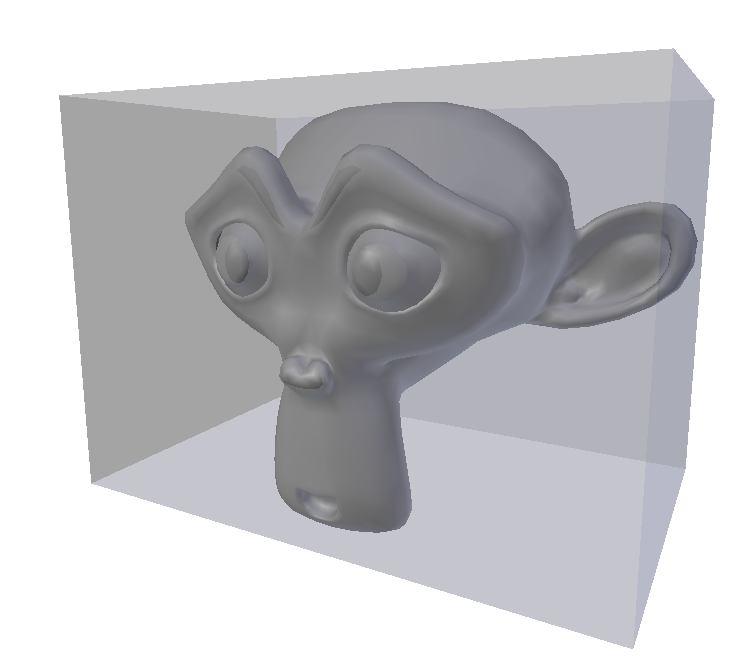
\includegraphics[width=\linewidth]{images/boiteenglobante}
		%\caption{Illustration d'une boite englobant un maillage quelconque}
		\label{boiteenglobante}
	\end{subfigureth}
	\qquad
	\begin{subfigureth}{0.35\textwidth}
		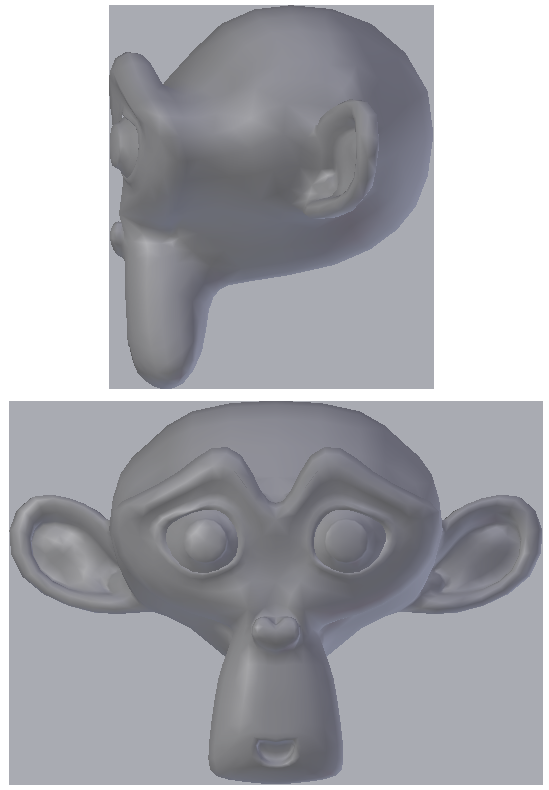
\includegraphics[width=\linewidth]{images/boiteenglobante2}
		%\caption{Illustration d'une boite englobant un maillage quelconque}
		\label{boiteenglobante2}
	\end{subfigureth}
	\caption{Illustration d'une boite englobant un maillage quelconque (Suzanne)}
\end{figureth}


\section{Calcul de rayons} \label{sect_rayon}


Le principe de la méthode utilisée est d'émettre depuis une source des rayons se propageant en ligne droite jusqu'à atteindre un triangle du maillage. Il est bon de noter que dans la nature, les ondes sonores peuvent suivre des trajectoires courbes à cause de certains paramètres comme les gradients de température ou la présence de vent. Néanmoins nous ferons l'approximation que la propagation se fait en ligne droite. Par ailleurs, les sources sonores telles que les instruments de musique ou la voix humaine ne sont pas omnidirectionnelles mais possèdent une répartition de l'énergie qui leur est propre. Comme précisé précédemment, notre étude se place dans le cas général d'une source ayant une répartition uniforme de son énergie dans toutes les directions de l'espace et pourra, dans un second temps, être enrichie par d'autres types de sources. 

Pour générer une émission omnidirectionnelle de rayons, nous avons dans un premier temps évalué l'utilisation d'une "\textit{Ico Sphère}" générée par Blender. L'idée est d'utiliser le centre comme origine et chaque vertice pour calculer le vecteur directeur des rayons. Effectivement, Blender propose dans ses objets de base une sphère formée par un icosaèdre régulier. Selon le rafinement voulu, Blender découpe chaque segment en son milieu et déforme la surface pour obtenir un modèle sphérique (voir fig. \ref{icosphere}). La répartition est donc uniforme puisque l'"\textit{Ico Sphère}" n'est composée que de triangles équilatéraux identiques. Cependant, Blender bride ces subdivisions à l'ordre 8, ce qui limite l'"\textit{Ico Sphère}" à 163842 points. Outre le fait que cette manipulation aurait largement ralenti Blender, nous souhaitons pouvoir traiter un nombre de rayons bien plus important et de valeur quelconque. Nous utilisons donc une sphère de Fibonacci afin de générer les vecteurs directeurs des rayons. 

\begin{figureth}
	\begin{subfigureth}{0.45\textwidth}
		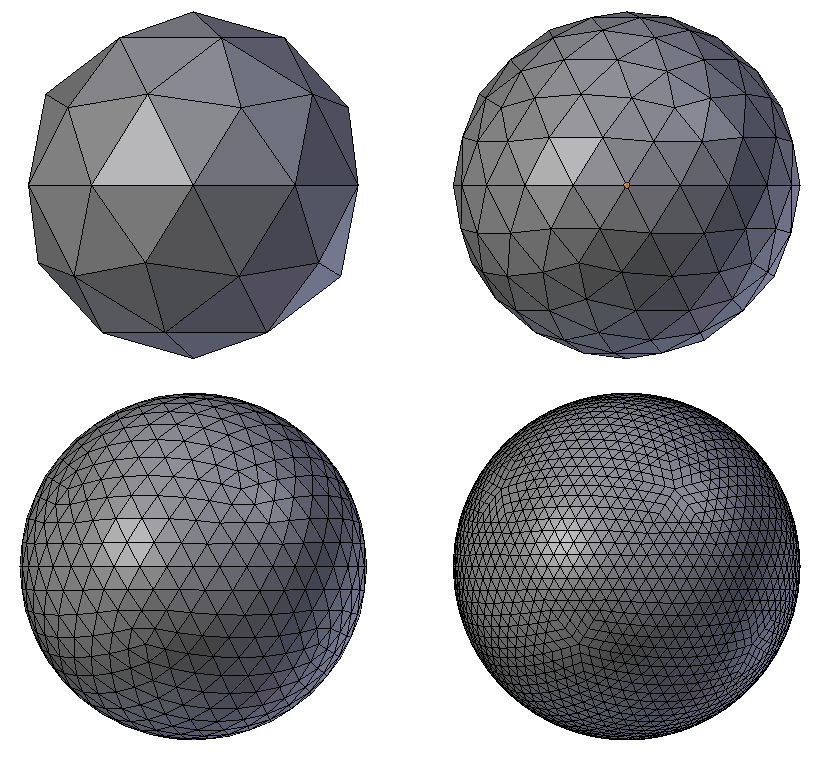
\includegraphics[width=\linewidth]{images/icosphere}
		\caption{Icosphère de Blender subdivisée 2, 3, 4 et 5 fois}
		\label{icosphere}
	\end{subfigureth}
	\qquad
	\begin{subfigureth}{0.45\textwidth}
		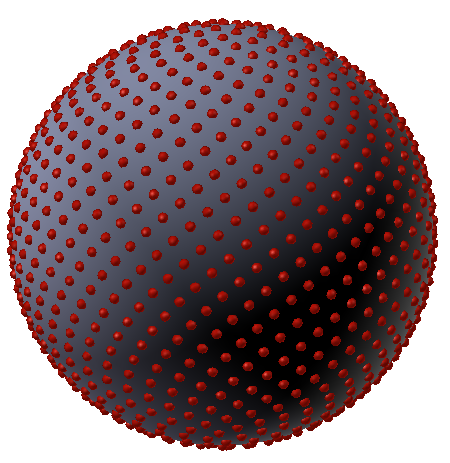
\includegraphics[width=\linewidth]{images/fibonacci}
		\caption[Sphère de Fibonacci]{Sphère de Fibonacci \footnotemark}
		\label{fibonacci}
	\end{subfigureth}
	\caption{Sphères permettant l'émission omnidirectionnelle de rayons}

\end{figureth}
\citefnt[fig. 1]{fibonacci}

On note $\Gamma$ le nombre d'or tel que :
\begin{equation}
\Gamma = \frac{1 + \sqrt{5}}{2}. \\
\end{equation}
%
Les coordonnées sphériques sont données par :
\begin{equation}
  \left \{
   \begin{array}{r c l}
\theta &=& \frac{2 \pi \times n}{\Gamma}  \pmod{2\pi},  \\
\phi &=& \arcsin{\left(\frac{2n}{N-1}-1\right)}, 
   \end{array}
   \right .
\end{equation}
%
avec : 
\begin{itemize}
\item $N$ : le nombre total de rayons,
\item $n \in[0, 1, 2, \ ... \ ,N-1]$ : le numéro du rayon.
\end{itemize}
%
A partir de ces coordonnées sphériques, on en déduit les coordonnées cartésiennes des vecteurs directeurs que l'on normalisera par la suite :

\begin{equation}
   \left \{
   \begin{array}{r c l}
x &=& \cos{\phi} \times \cos{\theta},  \\
y &=& \cos{\phi} \times \sin{\theta},  \\
z &=& \sin{\phi}.
   \end{array}
   \right .
\end{equation}


À l'initialisation nous émettrons donc $N$ rayons depuis le centre de l'objet source et dirigés dans toutes les directions de manière uniforme. Une énergie normalisée à $1$ leur est assignée de sorte que l'énergie totale vaille $N$ et ceux pour chaque bande de fréquence. L'algorithme va ensuite propager les rayons sur les parois et à chaque intersection les énergie vont être atténuées par l'absorption des parois (voir eq. \ref{eq_coeff_abs}). Tant que les huit énergies de d'un rayons ne sont pas toutes inférieures à une valeur seuil alors celui-ci continu de se propager. 

Pour tester les intersections entre les rayons et les parois nous utilisons l'algorithme de Möller-Trumbore \cite[p. 2-3]{moller} développé à la fin des années 90 d'après les travaux de J.Arenberg \cite{arenberg} et D.Badouel \cite[p. 390-393]{badouel} et reconnu pour être rapide et efficace. Il s'agit d'opérer un changement de base pour le vecteur directeur du rayon et d'exprimer le point d'intersection à l'aide de coordonnées barycentriques. Cela permet d'éviter de devoir travailler avec des équations de plans et soulage les calculs.

Nous cherchons donc l'intersection entre un rayons d'équation : 
\begin{equation}
R(t) = O + Dt,
\end{equation}
%
et une face triangulaire de sommets $ V_0, V_1, V_2$. \\

Un point T appartient au triangle si : 

\begin{equation} \label{eq_2moller}
T(u,v) = (1-u-v)V_0 + uV_1 + vV_2, \ \ \ \footnotemark
\end{equation}
\citefnt[eq. 2]{moller}
%
avec $(u,v)$ les coordonnées barycentriques tels que :
\begin{equation}
   \left \{
   \begin{array}{r c l}
u & \geqslant & 0,  \\
v & \geqslant & 0,  \\
(u+v) & \leqslant & 1.
   \end{array}
   \right .
\end{equation}
%
Ainsi, l'intersection entre le rayon et le triangle s'écrit :
\begin{equation}
O + Dt = (1-u-v)V_0 + uV_1 + vV_2, \ \ \ \footnotemark
\end{equation}
\citefnt[eq. 3]{moller}
%
avec $t$ la distance entre le point d'origine du rayon et le point d'intersection. D'après la règle de Cramer, nous pouvons réarranger cette équation sous la forme :
%
\begin{equation}
	\begin{bmatrix}
 	  -D, & V_1-V_0, & V_2-V_0
	\end{bmatrix}
	\begin{bmatrix}
 	 t \\
	 u \\
	 v
	\end{bmatrix}
	= O-V_0.
	\ \ \ \footnotemark
\end{equation}
\citefnt[eq. 4]{moller}
%
Ainsi, on aura :
\begin{equation}
	\begin{bmatrix}
 	 t \\
	 u \\
	 v
	\end{bmatrix}
	=
	\frac{1}{
	\begin{vmatrix}
 	  -D, & E_1, & E_2
	\end{vmatrix}
	}
	\begin{bmatrix}
 	 	\begin{vmatrix}
 		  T, & E_1, & E_2
		\end{vmatrix} \\
 	 	\begin{vmatrix}
 		  -D, & T, & E_2
		\end{vmatrix} \\
 	 	\begin{vmatrix}
 		  -D, & E_1, & T
		\end{vmatrix}
	\end{bmatrix}	.
	\footnotemark
\end{equation}
\citefnt[eq. 5]{moller}
%
avec : 
\begin{equation}
   \left \{
   \begin{array}{r c l}
E_1 &=&  V_1-V_0,  \\
E_2 &=&  V_2-V_0,  \\
T &=& O - V_0.
   \end{array}
   \right .
\end{equation}
%
Ce qui équivaut à : 
%
\begin{equation}
	\begin{bmatrix}
 	 t \\
	 u \\
	 v
	\end{bmatrix}
	=
	\frac{1}{
 	  (D \times E_2).E_1
	}
	\begin{bmatrix}
 		  (T \times E_1).E_2
 \\ 
 		  (D \times E_2).T
 \\
 		  (T \times E_1).D
	\end{bmatrix}	.
	\footnotemark
\end{equation}
\citefnt[eq. 6]{moller}

On peut alors connaitre toutes les faces que rencontre chaque rayon en conservant le point d'intersection pour le rayon le plus court. Effectivement, on admet que les faces peuvent absorber les rayons mais pas les transmettre donc le rayon s'arrêtera à la première face rencontrée. En pratique il peut y avoir des phénomènes de vibro-acoustique et de résonance qui peuvent transmettre le son à travers des parois. Nous pouvons négliger ces phénomènes notamment dans un cas comme le théâtre d'Orange dont l'épaisseur et la densité des murs est importante. Il est tout de même bon de noter que, pour cette raison, certains cas d'utilisation ne pourront pas être testés comme par exemple l'écoute dernière une porte ou sous l'estrade de bois.

\begin{figureth}
	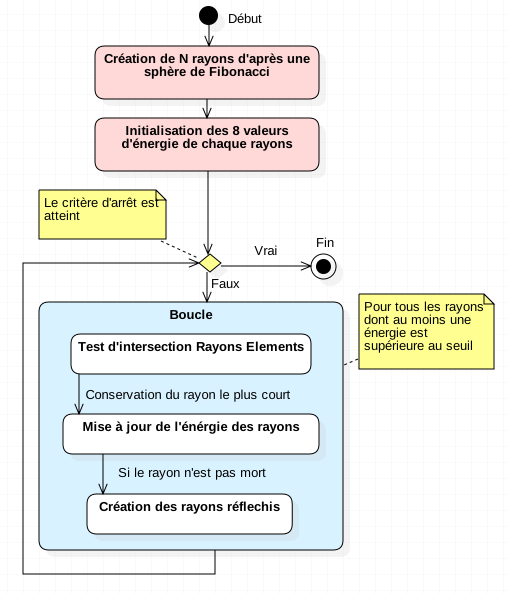
\includegraphics[width=0.7\linewidth]{images/DiagRay}
	\caption{Diagramme d'activité résumant le processus de création des rayons}
	\label{DiagRay}
\end{figureth}

Une fois que l'on sait sur quelle paroi chaque rayon va se réfléchir, on peut mettre à jour leurs énergies en les multipliant pour chaque bande de fréquence par $(1-\alpha_i)$, les $\alpha_i$ étant les coefficients d'absorption de la face rencontrée (voir section \ref{sect_lectMat}). La longueur totale du rayon doit être stockée afin de pouvoir prendre en compte l'absorption de l'air, de créer les sources-images (voir section \ref{sect_si}) et de calculer la \gls{rir}  (voir section \ref{sect_rir}). Il y a alors deux possibilités pour que le processus s'arrête : 
\begin{itemize}
	\item Les énergies des huit bandes de fréquence portées par le rayon sont toutes en dessous d'un seuil. En général, ce seuil est fixé à -60dB pour une source-image, ce qui assure que le son ne soit plus audible. Il faut donc résonner en terme de faisceau de "n" rayons pour déterminer le seuil limite d'un rayon.
	\item La distance totale parcourue par le rayon a dépassé le seuil déterminé par l'équation \ref{seuil_arret}. Cela assure que l'angle solide soit négligeable devant le rayon du récepteur et ainsi que la répartition discrète d'énergie puisse être considérée comme quasi-continue (voir section \ref{sect_discretise}).
\end{itemize}
%
Les rayons pour lesquels aucun de ces deux critères n'est atteint donnent alors naissance à un rayon réfléchi, les autres arrêtent de se propager. 


Pour calculer le vecteur directeur des rayons réfléchis, il suffit d'utiliser le vecteur normal à la face rencontrée (de norme 1) et d'utiliser la formule suivante :

\begin{equation}
\overrightarrow{r} - \overrightarrow{i} = 2 \times (-\overrightarrow{i}.\overrightarrow{n})\overrightarrow{n}.
\end{equation}

\begin{figureth}
	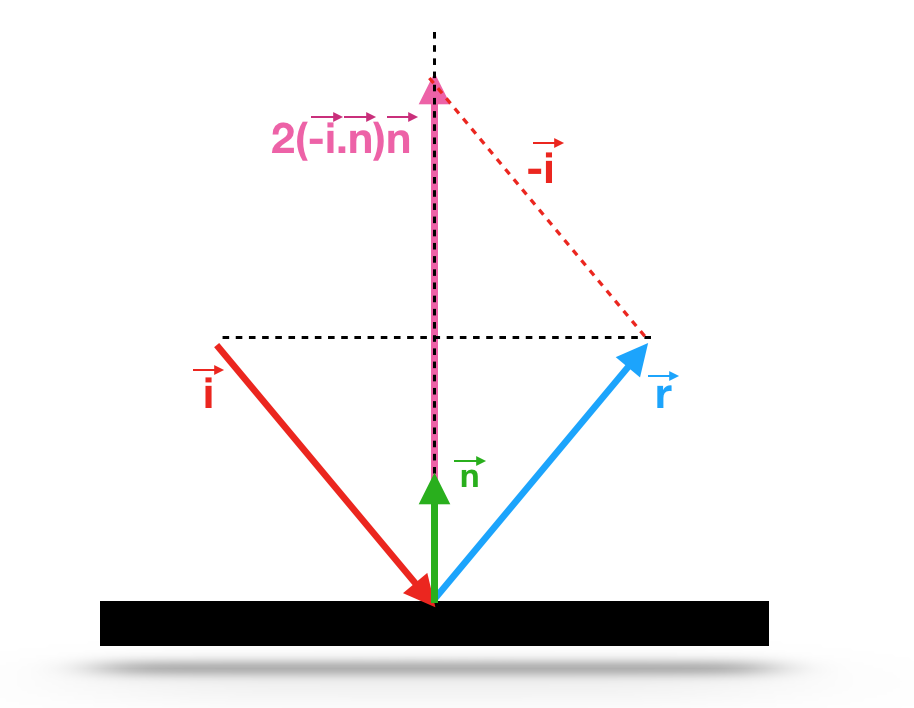
\includegraphics[width=0.6\linewidth]{images/rayRefl}
	\caption{Calcul d'un rayon réfléchi à partir d'un rayon incident et d'une normale}
	\label{rayRefl}
\end{figureth}

Nous pouvons ainsi mettre à jour les informations sur les rayons (origine et vecteur directeur) et boucler afin de propager ces rayons réfléchis vers de nouvelles faces. Notons tout de même que dans l'implémentation algorithmique il peut se produire des problèmes d'arrondis qui peuvent faire fuir des rayons (c'est à dire qu'ils ne rencontrent aucune face). Pour éviter cela, on modifie les conditions de l'équation \ref{eq_2moller} tel que :
\begin{equation}
   \left \{
   \begin{array}{r c l}
u & \geqslant & -\epsilon,  \\
v & \geqslant & -\epsilon,  \\
(u+v) & \leqslant & 1+\epsilon,
   \end{array}
   \right .
\end{equation}
avec $\epsilon = 10^{-5}$ (la précision machine étant de $10^{-6}$ pour une variable de type \textit{float}). De même, si un rayon tombe dans un coin, son rayon réfléchi pourra sortir du maillage. Pour éviter cela on aura :
\begin{equation*}
l = l- \epsilon,
\end{equation*}
avec $l$ la longueur du rayon.




\section{Calcul de sources-images} \label{sect_si}



\begin{figureth}
	\begin{subfigureth}{0.55\textwidth}
			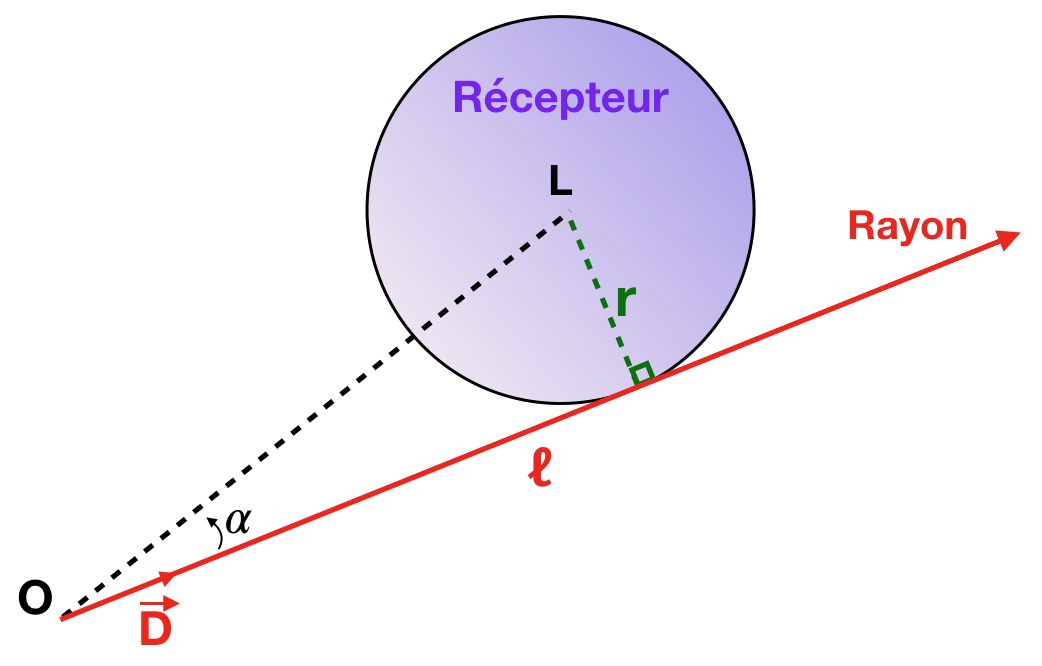
\includegraphics[width=\linewidth]{images/touche}
			\caption{Schéma d'un rayon qui passe en frontière de la sphère récepteur de rayon r}
			\label{touche}
		\end{subfigureth}
		\qquad
		\begin{subfigureth}{0.35\textwidth}
			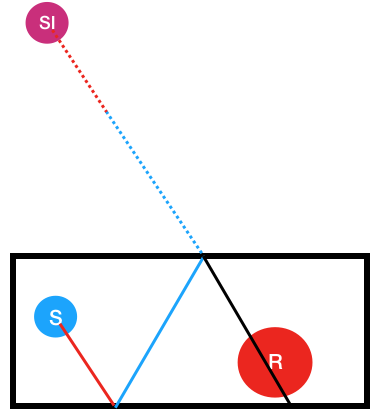
\includegraphics[width=\linewidth]{images/schema_SI}
			\caption{Schéma de la création d'une source image par réflexions successives d'un rayon sur les parois d'une salle}
			\label{schema_SI}
	\end{subfigureth}
\end{figureth}

A chaque itération, c'est à dire à chaque fois que les $N$ rayons sont entrés en contact avec une paroi et avant qu'ils ne soient réfléchis, on détermine ceux qui ont traversé le récepteur. Nous allons ainsi pouvoir ajouter au fur et à mesure des itérations de nouvelles sources-images. Pour savoir si un rayon (parmi les rayons qui n'ont pas atteint le critère d'arrêt) donne naissance à une source image, on vérifie dans un premier temps si le point d'origine du rayon est à l'intérieur de la sphère-récepteur:

\begin{equation}
||\overrightarrow{OL}|| \leqslant r,
\end{equation}
avec :
\begin{itemize}
\item$O$ : L'origine du rayon,
\item$L$ : Le centre du récepteur (Listener),
\item$r$ : Le rayon de la sphère récepteur.
\end{itemize}
%
Si c'est le cas, alors le rayon est perçu par le récepteur et une source image va être créée. Sinon, on vérifie si le rayon se dirige bien vers le récepteur. Pour cela il suffit de vérifier que :

\begin{equation}
\cos{\alpha} \geqslant 0,
\end{equation}
avec $\alpha$ l'angle entre le rayon de vecteur directeur $\overrightarrow{D}$ et $\overrightarrow{OL}$. Par ailleurs, on vérifie que le rayon est assez grand pour atteindre le récepteur (donc qu'il n'est pas interrompu par une paroi avant) :

\begin{equation}
||\overrightarrow{OL}|| \leqslant l,
\end{equation}
%
avec $l$ la longueur du rayon. Pour finir, on s'assure que le rayon intersecte bien la sphère-récepteur :

\begin{align}
\sin{\alpha} \times ||\overrightarrow{OL}||  \leqslant r 
\quad \Rightarrow \quad
\alpha  \leqslant \arcsin{\frac{r}{||\overrightarrow{OL}||}}
\end{align}

\begin{figure}[h]
\centering
	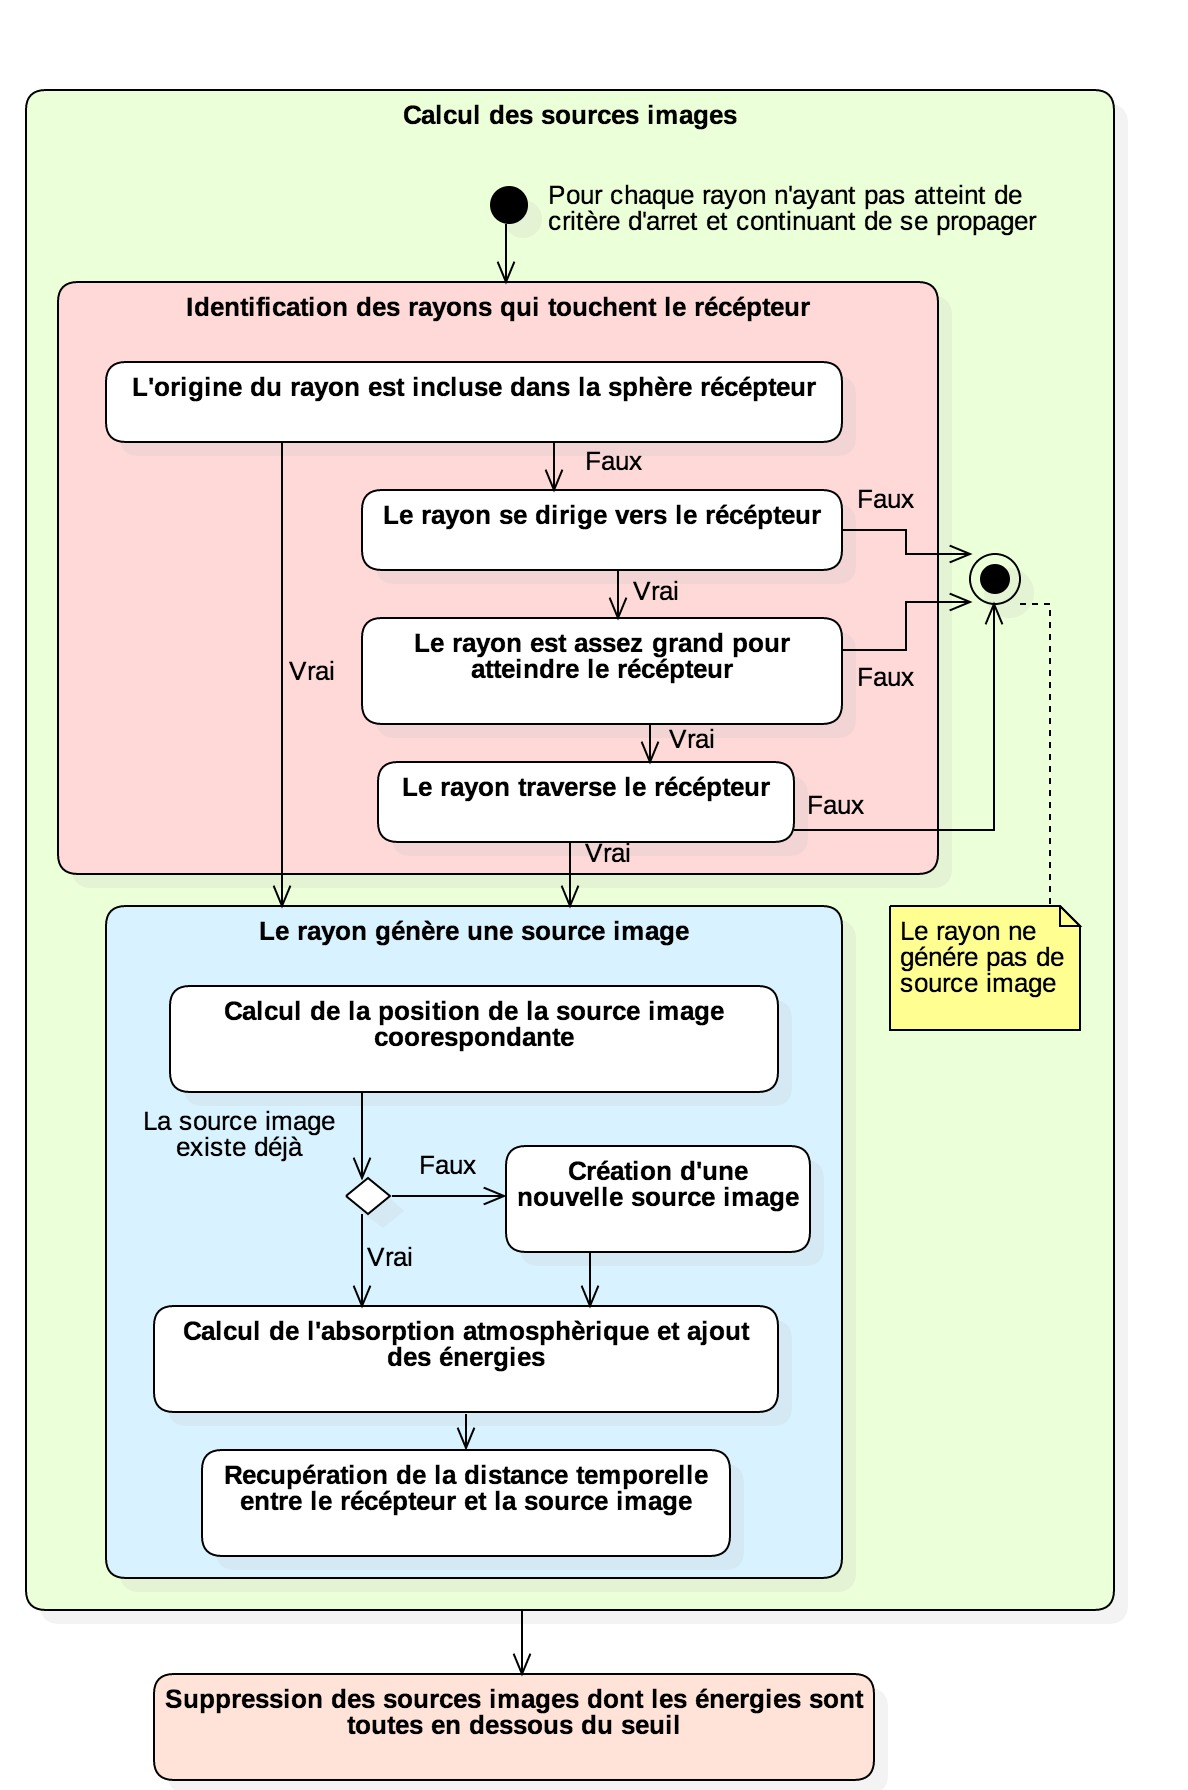
\includegraphics[width=0.7\linewidth]{images/DiagSi}
	\caption{Diagramme d'activité résumant le processus de création des sources-images}
	\label{DiagSi}
\end{figure}


Si ces conditions sont réunies, alors le rayon traverse bien le récepteur et une source-image est générée. Ses coordonnées sont obtenues en traçant un vecteur de même origine mais de sens opposé au rayon courant et dont la norme sera égale à la distance totale parcourue par le rayon avant sa dernière réflexion (voir fig. \ref{schema_SI}). On rétro-propage donc le rayon jusqu'à arriver à la source-image dont la position est le symétrique de la source par rapport à tous les plans rencontrés par le rayon. On assigne à cette source-image huit coefficients d'énergie correspondant aux coefficients d'énergie finaux du rayon, atténués par l'absorption de l'air sur le trajet total. Celle-ci est déterminée pour chaque bande de fréquence d'après les formules analytiques décrites dans la section \ref{sect_absAIr}. Le calcul des énergies se fait de la manière suivante :

\begin{equation}
E_{si, i} = E_{r, i} \times e^{-m_i \times l_{tot}},
\end{equation}
avec : 
\begin{itemize}
\item $E_{si, i}$ : L'énergie portée par la source image sur la i-ème bande de fréquence,
\item $E_{r, i}$ : L'énergie finale portée par le rayon sur la i-ème bande de fréquence,
\item $m_i$ : Le coefficient d'absorption de l'air sur la i-ème bande de fréquence (voir \ref{sect_absAIr}),
\item $ l_{tot}$ :La distance totale parcourue par le rayon entre la source et le récepteur.
\end{itemize}
%
Étant donné que tous les rayons qui se seront réfléchis sur une même paroi vont générer des sources-images en un même point, on peut sommer leur énergie. Il n'y aura donc qu'une seule source-image portant l'énergie de plusieurs rayons.

Pour finir, on assigne à chaque source-image une distance temporelle afin pouvoir tracer la réponse impulsionnelle :
\begin{equation}
 t_{tot} =  \frac{l_{tot}}{v},
\end{equation}
avec : 
\begin{itemize}
\item$ t_{tot}$ : le temps de parcours entre la source-image et le récepteur,
\item$v$ : la vitesse du son dans le milieu (air : 340m/s).
\end{itemize}


\section{Génération de réponse impulsionnelle} \label{sect_rir}

Disposant de la distance temporelle entre les sources-images et le récepteur, il est possible d'afficher les courbes d'énergie sonore en fonction du temps. Aussi, pour chaque bande d'octave nous sommons les énergies par tranches temporelles. Ces tranches sont déterminées par la fréquence d'échantillonnage $f_s$. Celle-ci devra être identique à celle du signal audio avec lequel la réponse impulsionnelle sera convoluée (voir section \ref{sect_TDS}). Ainsi :
\begin{align}
nb_{ech} = f_s \times t_{max}, 
\end{align}
avec : 
\begin{itemize}
\item$nb_{ech}$ : le nombre total d'échantillon,
\item$f_s$ : la fréquence d'échantillonnage,
\item$t_{max}$ : le temps de parcours de la source image la plus éloignée,
\end{itemize}

%
et pour chaque bande d'octave on somme les énergies par échantillon. On a alors : 
%
\begin{align}
E_{i} =  \sum{E_j},
\end{align}
tel que la partie entière du produit  $(t_j \times f_s) = i$
et avec : 
\begin{itemize}
\item$E_{i}$ : l'énergie du $i^e$ échantillon,
\item$E_j$ et $t_j$ : respectivement l'énergie et temps de parcours de la $j^e$ source-image.
\end{itemize}


 \begin{figureth}
	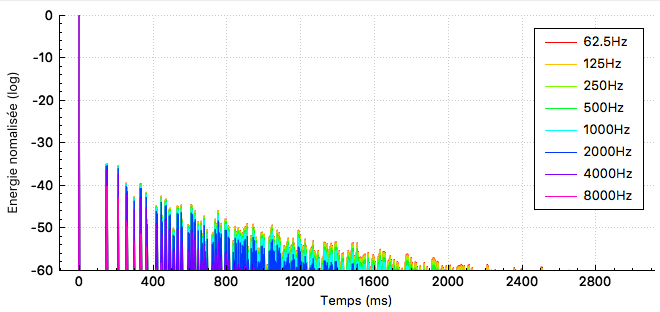
\includegraphics[width=0.9\linewidth]{images/rir}
	\caption[Réponse impulsionnelle d'un cube]{Exemple de \gls{rir} pour un cube de 50m d'arrête, une source et un récepteur de 20m de diamètre situés au centre, un million de rayons et une fréquence d'échantillonnage de 44100Hz}
	\label{rir}
\end{figureth}

Typiquement, pour une fréquence standard de 44100Hz chaque échantillon sommera les énergies des sources-images par tranches de $22,7\mu s$. Les énergies seront ensuite normalisées pour obtenir la \gls{rir} (voir fig. \ref{rir}).

On a vu dans les sections \ref{sect_discretise} et \ref{sect_rayon} que la mesure pouvait être arrêtée avant d'atteindre le seuil limite d'audition, c'est à dire -60dB. Ce cas se présente lorsque le nombre de rayons est faible, lorsque le diamètre de la sphère récepteur est petit ou bien lorsque les rayons ont une longue distance à parcourir avant d'être suffisamment atténué (dans le cas d'une pièce fermée avec des parois très réfléchissantes par exemple). Dans ce cas, la \gls{rir} doit être complétée pour pouvoir atteindre le niveau d'énergie minimum demandé (-60dB). Pour cela, chaque courbe va être prolongée par régression linéaire afin de générer de manière statistique la queue de réverbération. D'après Sabine \cite[]{sabine} \\
A completer ...



\section{Auralisation}
 \label{sect_TDS}

L'analyse de résultats d'une étude acoustique peut parfois être délicate et difficile pour les personnes extérieurs au milieu. Le résultat final qui pourra être analysé par le plus grand nombre est le signal audio de sortie. Même si l'analyse d'un signal audio nécessite une grande finesse auditive, elle présente pour avantage d'être accessible par une simple écoute. Pour obtenir le son réverbéré, il s'agit de convoluer le signal d'origine avec les \gls{fir}. Un \gls{fir} est une \gls{rir} exprimé en pression telle que :

\begin{equation}
P = \sqrt{E},
\end{equation}
avec : 
\begin{itemize}
\item $P$ : La pression sonore normalisée,
\item $E$ : L'énergie normalisée.
\end{itemize}

Convoluer ces signaux revient à multiplier point par point le fichier audio avec les \gls{fir} dans le domaine de Fourier (fréquenciel).
On utilise pour cela des fichiers au format \gls{wav}. Dans le cas de longs signaux, il est judicieux d'utiliser une convolution partitionnée afin de réduire le stockage de données et accélérer les calculs \cite[2. Algorithm overview ]{partition}. 

L'algorithme mis en place fonctionne de la manière suivante (voir fig. \ref{DiagTdS}) :
\begin{figureth}
	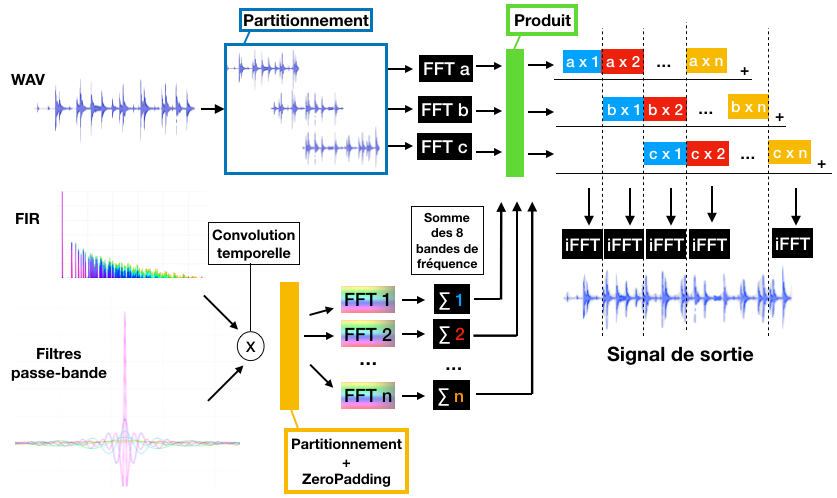
\includegraphics[width=\linewidth]{images/DiagTdS}
	\caption{Schéma du processus de convolution partitionnée}
	\label{DiagTdS}
\end{figureth}

Premièrement, on fixe la longueur des partitions à $n$ échantillons tel que $n$ soit une puissance de 2 (typiquement 1024). Dans un premier temps, le signal audio est découpé par tranches de $n$ échantillons et chaque tranche recouvre la précédente sur la moitié de sa taille. Chacune d'entre elles est ensuite passées dans le domaine spectral par \gls{fft}. Dans un second temps, les \gls{fir} sont convolués temporellement à des filtres passe-bande (voir fig. \ref{filtres}), c'est à dire que chaque pic des \gls{fir} sera multiplié par le filtre passe-bande de la fréquence correspondante. Les huit signaux de sortie sont alors découpés par tranches de $n/2$ échantillons que l'on fait précéder de $n/2$ zéros. Ce procédé se nomme "\textit{ZeroPadding}" et permet d'éviter les effets de crénelage (\textit{aliasing}) lors de la convolution de deux signaux. En effet, les spectres des signaux présentent sur leur partie négative un repliement qui apporte de l'information redondante lors de la convolution. C'est pour cette même raison que les partitions du signal audio ont un recouvrement de $n/2$ échantillons. Ainsi, seuls les $n/2$ derniers échantillons du résultat de convolution sont utiles. Avant de pouvoir effectuer cette opération il faut passer les filtres dans le domaine spectral et sommer les huit bandes de fréquence. Une par une les partitions du signal audio sont convoluées aux filtres et à chaque nouvelle partition, on décale le résultat de $n/2$ échantillons. On pourra alors sommer les résultats et effectuer une transformée de Fourier inverse pour récupérer le signal de sortie. Celui-ci sera identique au signal d'entrée à la différence qu'il sera réverbéré, c'est à dire que chaque pic de la \gls{rir} répétera le signal d'entrée en écho.

\begin{figureth}
	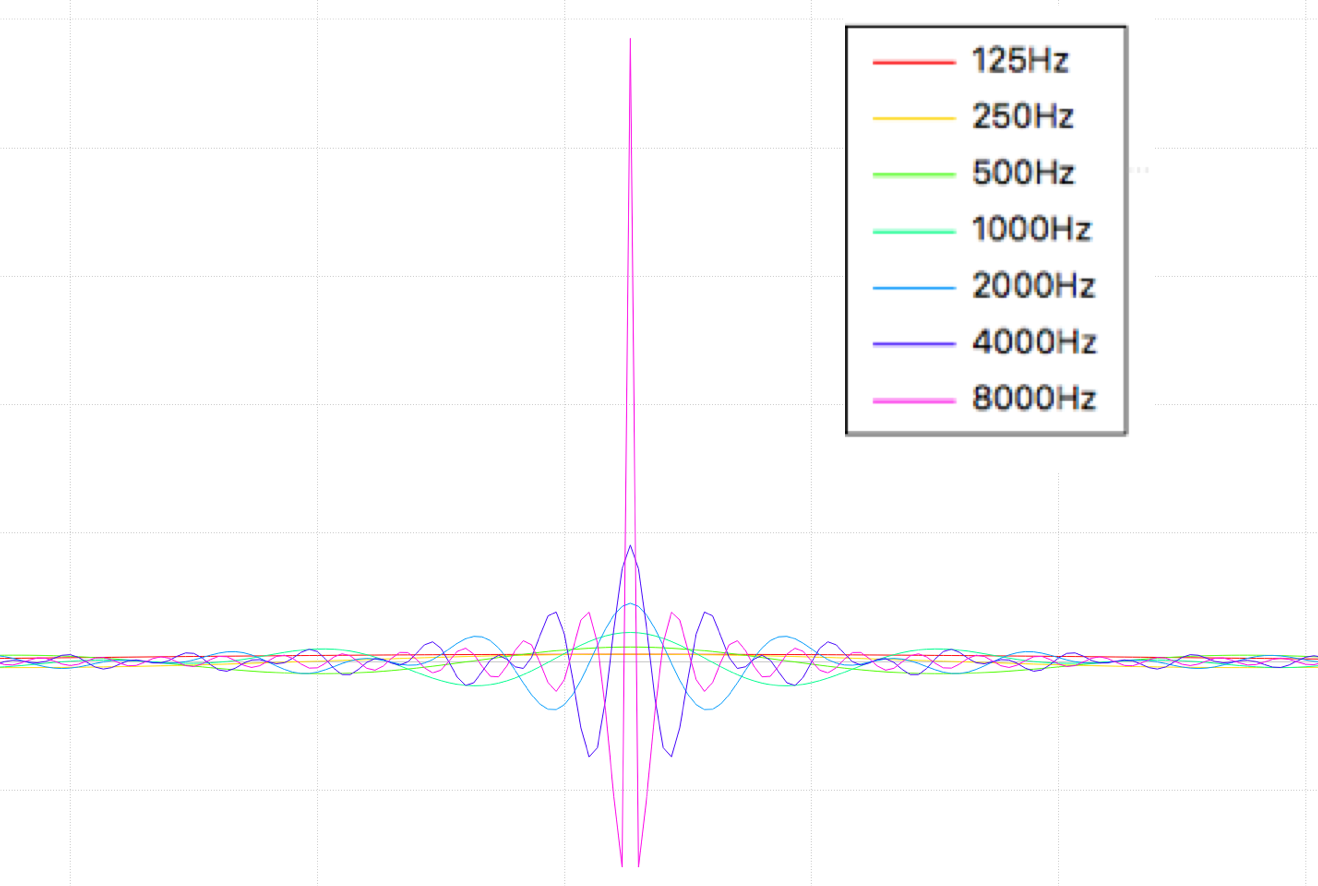
\includegraphics[width=0.9\linewidth]{images/filtres}
	\caption{Filtres fréquenciels passe-bande}
	\label{filtres}
\end{figureth}

Dans un futur développement il sera possible de générer une \gls{rir} pour l'oreille gauche et une autre pour l'oreille droite afin d'avoir une signal binauralisé. L'écoute pourra alors dépendre des angles d'azimut et d'élévation orientant le regard de l'auditeur. Ainsi, le son sera spatialisé et l'étude acoustique pourra prendre une nature immersive. Celle-ci pourra être renforcée par l'utilisation d'un casque muni d'un \textit{Head-Tracker} afin de corriger les angles d'observation en temps réel \cite{myBino}. Ce type de casque possède un gyroscope qui actualise la direction du regard en temps réel et permet d'augmenter considérable la sensation immersive. 

%\section{Signal binaural avec head-tracker}
%
%A faire éventuellement ....






\chapter{Optimisation algorithmique}
	\citationChap{
	Un pessimiste voit la difficulté dans chaque opportunité, un optimiste voit l'opportunité dans chaque difficulté.
	}{Winston Churchill}
	\minitoc
	\newpage
	
\section*{Introduction} \label{sect_complexite}

Afin de pouvoir qualifier les performances de l'algorithme, il est d'usage d'en mesurer la \gls{complexite}. Ce coefficient vise à analyser et qualifier le temps de calcul d'un algorithme. Pour rappel les grandes étapes de l'algorithme qui font appel à des boucles d'itérations importantes sont les suivantes :
\begin{itemize}
\item lecture du maillage,
\item intersection des rayons et des faces,
\item création des sources-images.
\end{itemize}
On note $N$ le nombre de rayons et $M$ le nombre de faces du maillage. Nous allons donc pouvoir analyser la complexité de ces différentes étapes. La lecture du maillage ne dépend que du nombre de faces ; la complexité de cette opération est donc linéaire de type $O(M)$. Par ailleurs cette étape n'est réalisée qu'une fois à l'initialisation. La création des sources-images ne dépend que du nombre de rayons sera elle aussi de complexité linéaire en $O(N)$. Celle-ci se produit en boucle tant que tous les rayons n'ont pas atteint le seuil d'arrêt. Néanmoins on ne peut pas en déterminer le nombre de boucles car celui-ci dépend de la géométrie de la salle et des matériaux. Effectivement plus la salle est grande et plus les matériaux sont absorbants, plus vite s'arrêtera la boucle. 

L'étape la plus complexe est la boucle d'itération sur le calcul des intersection entre les rayons et les faces. Lors de cette étape, chaque rayon est testé avec chaque face. La complexité de cet algorithme est donc quadratique en $O(N \times M)$. Il s'agit de l'étape critique de la méthode et la plus chronophage. Pour vérifier cela, nous mesurons le temps de calcul des intersections rayons-faces pour une itération (voir fig. \ref{complexite00} et tab. \ref{tabComplexite}). Ce test est effectué sur un MacBook de procésseur 2,7GHz Intel Core i5 avec 8Go de RAM DDR3. La géométrie utilisée est un tétraèdre dont le nombre de faces est multiplié par deux à chaque mesure.


 \begin{figureth}
	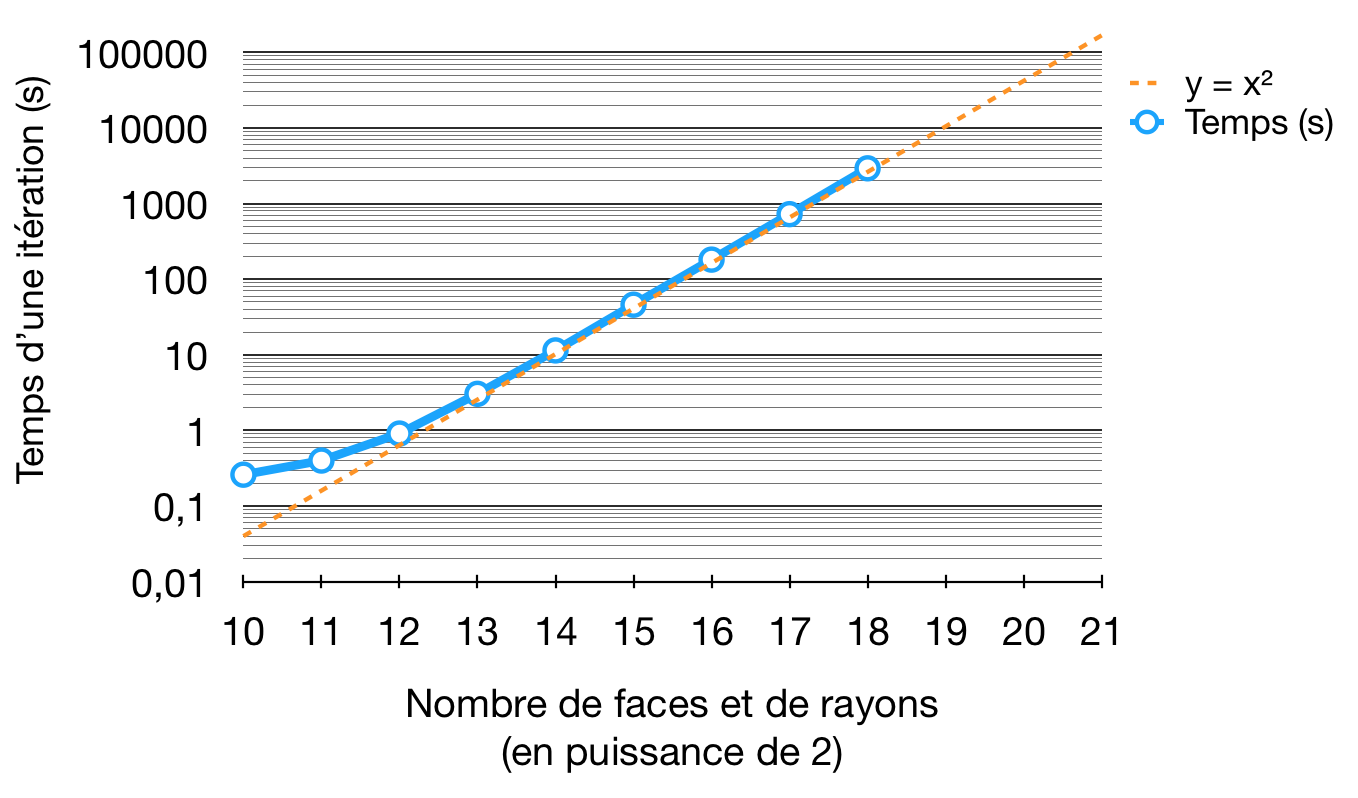
\includegraphics[width=0.8\linewidth]{images/complexite00}
	\caption{Courbe de complexité donnant le temps (s) d'une itération pour N=M en échelle logarithmique}
	\label{complexite00}
\end{figureth}

La courbe \ref{complexite00} illustrant le temps de calcul en faisant varier le nombre N de rayons et le nombre M de faces tel que $N=M$ comporte bien une pente de 2 en échelle logarithmique. Effectivement :
%
\begin{equation}
T \propto N^2 \qquad \Rightarrow \qquad \ln{(T)} \propto 2 \ln{(N)}.
\end{equation}
On constate comme prévu que le temps de calcul évolue comme le produit du nombre de faces par le nombre de rayons ce qui donne bien une complexité quadratique. 

Par ailleurs en fixant d'une part le nombre de face et d'autre part le nombre de rayons on constate que le temps augmente bien linéairement par rapport à chacun de ces paramètres (voir fig . \ref{complexite0}).

 \begin{figureth}
	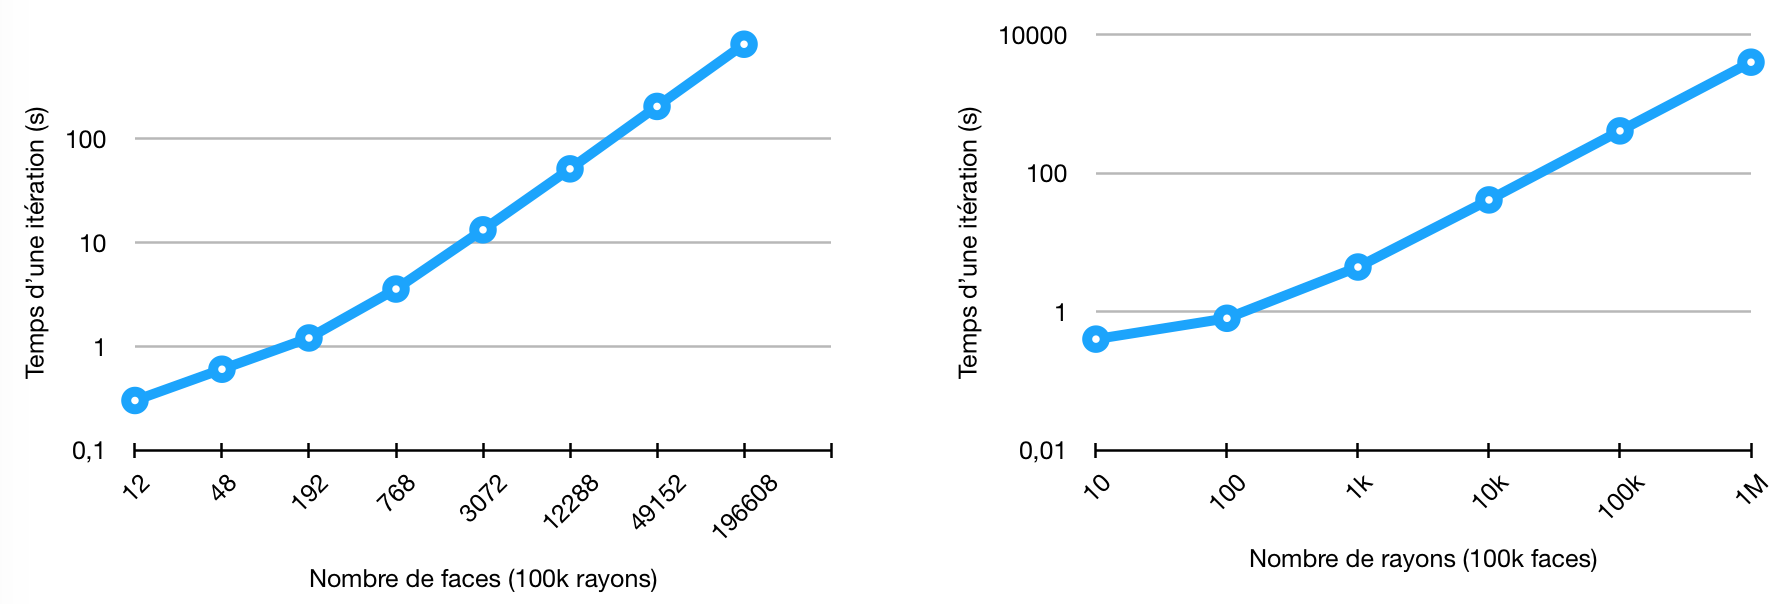
\includegraphics[width=\linewidth]{images/complexite0}
	\caption{Courbes de complexité donnant le temps (s) d'une itération en échelle logarithmique}
	\label{complexite0}
\end{figureth}


Dans le cas du théâtre d'Orange, le nombre de faces est supérieur à 100~000 éléments et le nombre de rayons à émettre doit être très important compte tenu de la taille du bâtiment (voir section \ref{sect_discretise}). En testant une géométrie simplifiée du bâtiment, nous constatons que son \gls{RT60} est de l'ordre de 2 secondes. Il faudra donc pouvoir réaliser des mesures pour des rayons d'environ 700m de long. Or d'après l'équation \ref{eq_dmax} :

\begin{equation}
N > n\left(\frac{2d}{r}\right)^2.
\end{equation}

Pour une sphère de mesure de quelques mètres (celle-ci ne doit pas trop s'étendre afin que la mesure reste localisée) et $n$ de l'ordre d'une centaine de rayons, il faudra que le nombre total de rayons $N$ soit supérieur à 50 millions. En prolongeant la courbe de la figure \ref{complexite0} on obtient un temps de calcul d'une trentaine d'heure, ce qui n'est pas acceptable pour entrer dans le cahier des charges. Nous devons donc optimiser l'algorithme afin de résoudre ce problème.

\section{Méthode d'octree}
\subsection{Principe général} \label{sect_octree_gene}

Comme nous l'avons vu précédemment, les maillages que nous devons traiter peuvent comporter plusieurs dizaines, voire centaines de milliers d'éléments. Les algorithmes permettant de gérer ce genre de cas utilisent souvent des méthodes dites de "diviser pour régner" (\textit{divide and conquer}). Cela permet, notamment dans des environnements 3D de pré-trier les données afin de ne réaliser les calculs couteux en temps que sur une quantité de données restreinte. %Dans notre cas, l'utilisation d'un arbre nous permettra de ne tester les interactions qu'entre certains rayons et certaines faces : ceux et celles qui seront situés dans la même subdivision de l'espace. 

\begin{figureth}
	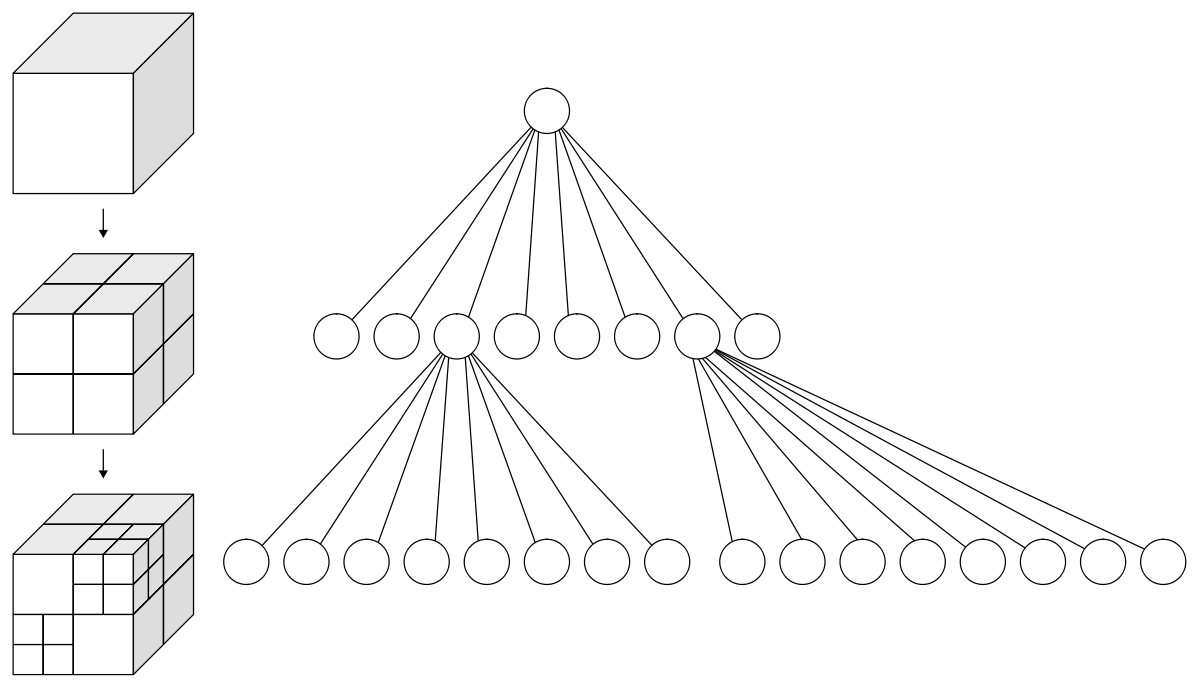
\includegraphics[width=0.6\linewidth]{images/octree}
	\caption{Illustration du principe d'\gls{octree}. Subdivision d'un cube en "octants" (gauche) et l'arbre correspondant (droite)}
	\label{octree}
\end{figureth}

Il existe plusieurs types d'arbres permettant l'optimisation des calculs par partitionnage de données. On pourra citer l'exemple bien connu des arbres binaires qui subdivisent les données en deux de manière récursive \cite[p. 318–348]{binaire}. Nous avons choisi d'utiliser un arbre assez similaire à la différence prés qu'il sépare l'espace en 2 sur chacune des dimensions de l'espace et crée des subdivisions de taille identiques alignées avec les axes. Chaque itération découpe la partition de l'espace précédente en 8 (soit $2^3$) ce qui donne le nom d'\gls{octree} à ce procédé \cite[p. 5]{octree}. 

Le principe général consiste à créer une boite cubique dite "boite-mère" contenant l'ensemble des éléments du maillage, c'est à dire l'ensemble des faces triangulaires. Cette boite-mère est alors subdivisée pour créer huit "boites-filles" de taille identique qui elles-mêmes vont être subdivisées en huit boites-filles, etc (voir fig. \ref{octree}). De manière récursive, chaque élément contenu dans une boite-mère va être rangé dans la boite-fille qui le contient. On descend de cette façon dans l'arborescence de l'arbre jusqu'à atteindre une condition d'arrêt. Typiquement, l'\gls{octree} s'arrête lorsque plus aucune boite-fille ne contient plus de $n$ éléments. Les boites sont donc raffinées de la même manière que le maillage (voir fig. \ref{octreeSuzanne}) puisque que les boites vides ne génère pas de boites-filles.

\begin{figureth}
	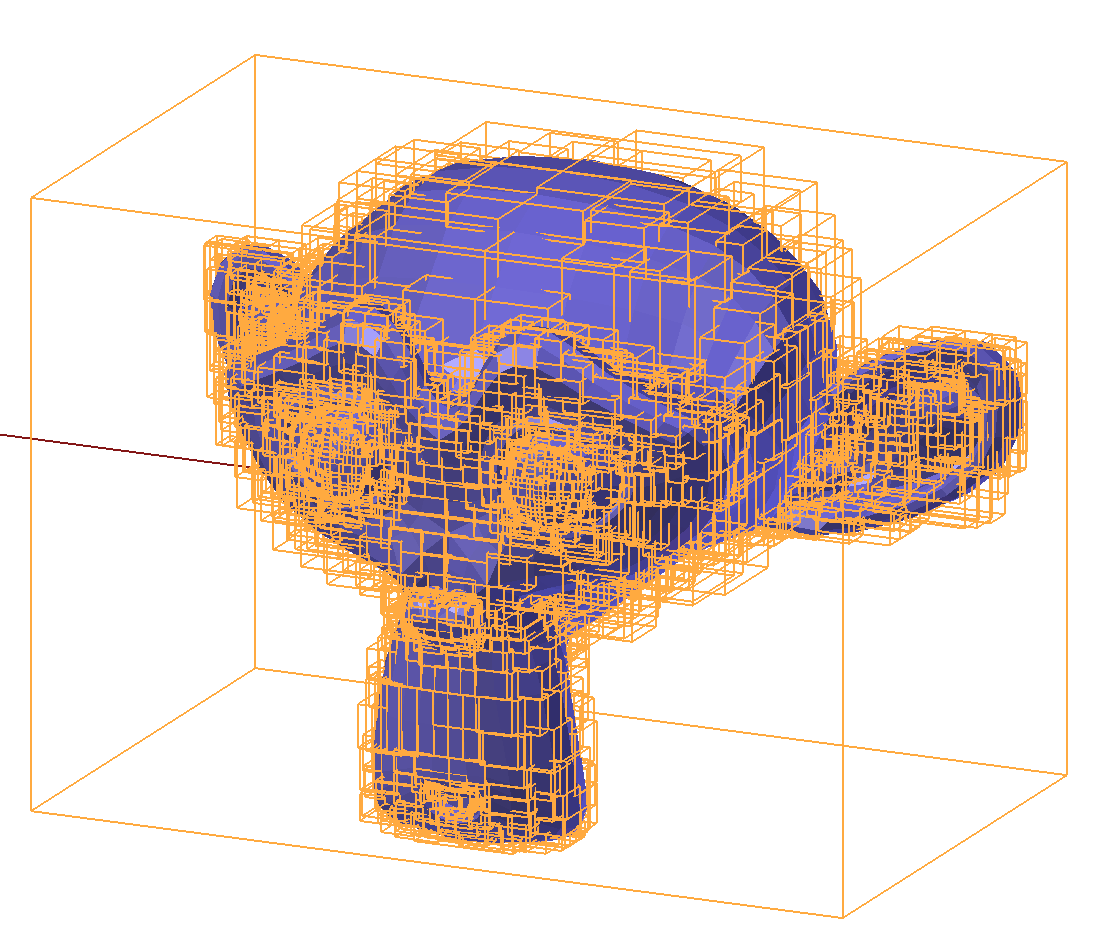
\includegraphics[width=0.6\linewidth]{images/octreeSuzanne}
	\caption{Suzanne triée dans un \gls{octree}}
	\label{octreeSuzanne}
\end{figureth}

Vérifions si ce système de tri permet de réduire la complexité du calcul. Nous avons vu que l'étape la plus chronophage de l'algorithme est l'interaction des rayons et des faces. Avec le partitionnage spatial de l'\gls{octree} nous ne testons que les rayons et les faces d'une même boite. Nous nommons \textit{objet} : un rayon ou une face. Dans un premier temps, voyons la complexité de la répartition des \textit{objets} dans les boites. Nous nous plaçons dans le cas idéal où N \textit{objets} sont repartis de manière uniforme dans l'espace. On nomme \textit{opérations} le rangement des \textit{objets} dans les boites. On note $p$ le nombre d'étages de l'\gls{octree}. Pour $p=0$, c'est à dire lorsque l'\gls{octree} n'est composée que de sa boite-racine, la boite-mère contient N \textit{objets}. Pour $p=1$ il faut ranger N élément dans 8 boites-filles. Il y aura donc $8N$ \textit{opérations}. A l'étage suivant, chaque boite-fille contenant $\frac{N}{8}$ \textit{objets} devient alors un boite mère traitée comme précédemment. Ainsi il faut $8$ \textit{opérations} par boite-mère pour ranger leurs $\frac{N}{8}$ \textit{objets}. Nous avons donc à cette étape :
%
\begin{center}
$8\times 8\times \frac{N}{8}$ = $8N$ \textit{opérations}.
\end{center}
%
De la même manière à l'étape suivante on aura :
\begin{center}
$8^3\frac{N}{8^2}$ = $8N$ \textit{opérations}.
\end{center}
%
Que l'on peut écrire dans le cas général :
\begin{equation} \label{operation}
8^p\frac{N}{8^{p-1}} = 8N \ \textit{opérations}.
\end{equation}
%
On constate qu'il faut faire $p$ fois $8N$ \textit{opérations} pour arriver à l'étage $p$. Il y aura donc $p \times 8N$ \textit{opérations} au total. %qu'à chaque étage on a un nombre constant d'\textit{opérations} proportionnel au nombre d'\textit{objets} à ranger dans les boites et que le nombre total d'\textit{opérations} est proportionnel à $p.N$.

Voyons maintenant comment déterminer $p$. Nous nous plaçons dans le cas où les boites du dernier étage ne contiennent qu'un unique \textit{objet}. Nous avons donc autant de boites que d'\textit{objets}. Ainsi :

\begin{align}  \label{nbEtage}
8^p &= N \nonumber, \\
p.\ln{8} &= \ln{N} \nonumber, \\
p &= \frac{1}{\ln{8}}\ln{N}.
\end{align}
%
Le nombre total d'\textit{opérations} $C$ est donc :
\begin{equation}
C = p.8N = \frac{8N}{\ln8}\ln{N}.
\end{equation}
Le rangement des \textit{objets} dans les boites est donc proportionnel à $N.\ln{N}$. À cela il faudra ajouter les calculs des intersections rayons/faces qui ne sont fait que $N$ fois, c'est à dire une fois par boite (puisqu'on n'a qu'un rayon et qu'une face par boite). La complexité totale devient :
\begin{equation}
C_{tot} = p.8N = \frac{8N}{\ln8}\ln{N} + N.
\end{equation}

Dans le cas général où les \textit{objets} ne sont pas répartis de manière uniforme, la démonstration est plus complexe. Effectivement, on ne peut pas prédire quelles boites vont être vides avant les autres et donc combien il y aura de boites par étages (voir fig. \ref{octree}). Cela est dû au fait que l'espace est divisé en $8^p$ à chaque étage et que selon la répartition des éléments certaines boites vont se retrouver vide et ne plus se subdiviser. La démonstration générale pourrait par contre fonctionner dans le cas d'un arbre binaire par exemple puisque le découpage dans l'espace se fait de manière à avoir un nombre équivalent d'éléments dans chaque boite quelque soit leur répartition. L'équation \ref{operation} donne :

\begin{center}
$2^p\frac{N}{2^{p-1}}$ = $2N$ \textit{opérations}.
\end{center}
On obtient alors :
\begin{equation}
C = p.2N = \frac{2N}{\ln2}\ln{N}.
\end{equation} 
Or, comme $\frac{2}{\ln2} > \frac{2}{\ln2}$ il faudra descendre plus loin dans les étages de l'arbre ce qui en pratique peut s'avérer être plus coûteux en temps.

De la même manière, en revenant au cas de l'\gls{octree} il pourra être plus judicieux de ne pas garder un unique \textit{objet} par boite dans le dernier étage mais plutôt d'arrêter l'arbre lorsque les boites possèdent toutes moins de $n$ \textit{objets}. L'équation \ref{nbEtage} devient :

\begin{equation} 
8^p = \frac{N}{n}.
\end{equation}
%
Ainsi :
\begin{align}
p.\ln{8} &= \ln{N} -  \ln{n}, \nonumber \\
p &= \frac{1}{\ln{8}}\ln{N} -  \frac{\ln{n}}{\ln{8}}, 
\end{align}
et
\begin{align}
C &=  p.8N = \frac{8N}{\ln8}\ln{N} - \frac{\ln n }{\ln8}8N.
\end{align}

Pour obtenir la complexité totale il faut ajouter le nombre d'opérations qu'il faut pour calculer les intersection rayons/faces par boite, c'est à dire $n^2$. On obtient :
\begin{equation}
C_{tot} = \frac{8N}{\ln8}\ln{N} - \frac{\ln n }{\ln8}8N + n^2.
\end{equation}
Le nombre d'étage nécessaire diminue donc d'un terme constant lié à $n$ et pour $n << N$ le temps de calcul sera proportionnel à ($aN\ln{N} + bN + c$) avec $a$, $b$ et $c$ des constantes non significatives. La complexité est donc en $O(N.\ln{N})$.



\subsection{Implémentation}


\begin{figureth}
	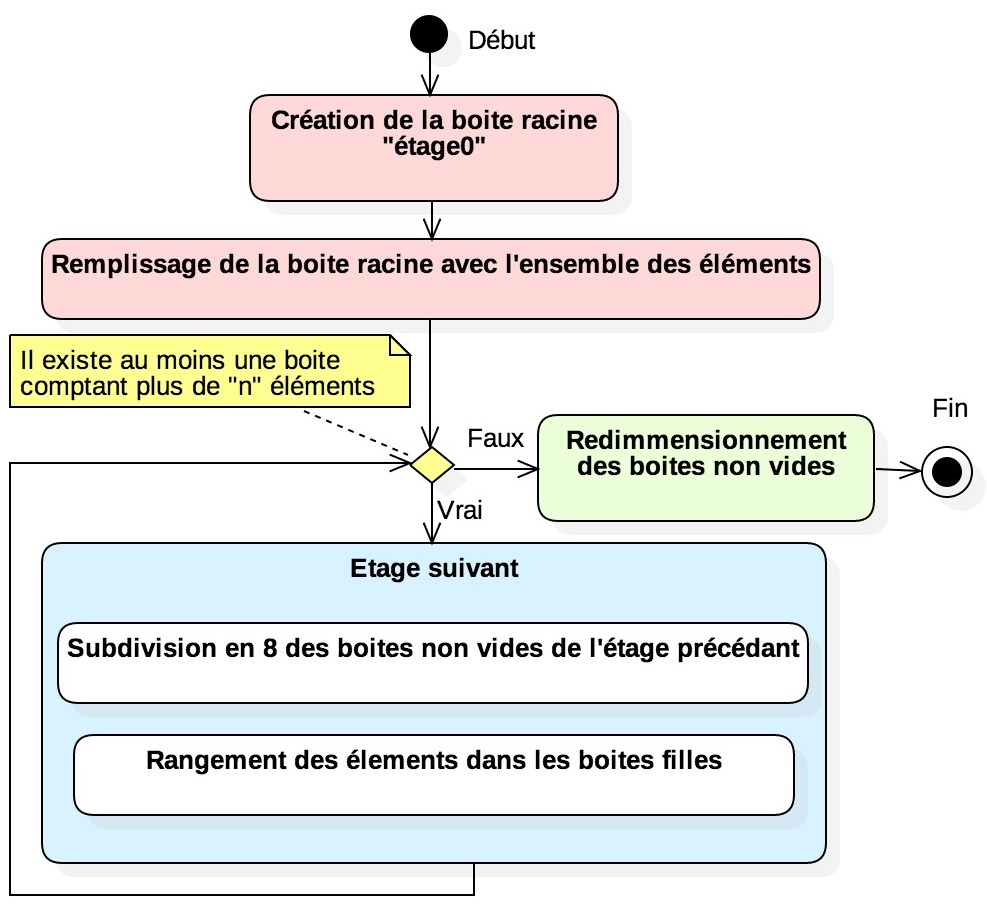
\includegraphics[width=0.7\linewidth]{images/DiagOctree}
	\caption{Diagramme d'activité résumant le processus de création d'un arbre d'octree}
	\label{DiagOctree}
\end{figureth}

L'algorithme a été développé comme décrit sur la figure \ref{DiagOctree}). Une première boite cubique englobant le maillage dans sa globalité est créée. On y associe les indices de l'ensemble des faces puisqu'elles sont toutes contenues dans cette boite-racine. On va ensuite, de manière récursive descendre dans des étages successifs. Passer de l'étage $p$ à l'étage $p+1$ revient à découper toutes les boites non-vides de l'étage $p$ en huit boites-filles de tailles égales qui deviendront à leur tour les boites-mères de l'étage $p+1$. Les indices des faces assignés à une boite-mère sont répartis dans les huit boites-filles. Pour savoir quel face appartient à quelle boite, on utilise les coordonnées du centre de la face. Effectivement, une face peut géométriquement rencontrer plusieurs boites mais il est nécessaire de les considérer comme ponctuelle afin qu'une face ne puisse se retrouver que dans une boite à la fois. La boucle récursive s'arrête lorsque les boites possèdent toutes moins d'éléments qu'une valeur seuil. Ainsi nous nous assurons que l'\gls{octree} se raffine de la même manière que le maillage et que chaque boite ne contient qu'un faible nombre d'éléments.


Il reste néanmoins une dernière étape qui permettra de s'assurer que les rayons rencontrent les bonnes faces. Il s'agit de redimensionner les boites non-vides pour que cette fois, elles englobent bien géométriquement les faces qu'elles contiennent.


À chaque itération, on va alors pouvoir répartir les rayons dans l'\gls{octree} (voir nouveau diagramme d'activité des rayons, fig. \ref{DiagRay2}). Pour cela, les rayons sont assignés aux boites qu'ils intersectent à partir de la boite-racine et en descendant dans l'arborescence de chaque branche. De la même manière que pour les triangles, les rayons sont testés avec des boites-filles que s'ils ont bien intersecté la boite-mère correspondante. Pour savoir si l'indice d'un rayon doit être assigné à une boite, nous utilisons un algorithme optimisé d'intersection Rayon/Boite \cite{AABB}. La particularité des boites d'un \gls{octree} est qu'elles sont toutes alignées selon les axes du repère cartésien. On appel communément ce type de boite \gls{AABB} en opposition aux \gls{OBB}. Nous allons donc utiliser cette propriété pour vérifier si un rayon intersecte une boite. Pour cela rappelons qu'un rayons peut s'écrire sous la forme : 
\begin{equation}
f(t) = D \times t + O
\end{equation}
avec :
\begin{itemize}
\item $D$ : le vecteur directeur du rayon de coordonnées $(D_x ; D_y ; D_z)$,
\item $O$ : le point d'origine du rayon de coordonnées $(O_x ; O_y ; O_z)$.
\end{itemize}

On peut également exprimer les plans délimitant la boite de type \gls{AABB} par les équations suivantes :
\begin{align*}
f(t) &= X_{min}  \\
f(t) &= X_{max}  \\
f(t) &= Y_{min}  \\
f(t) &= Y_{max} \\
f(t) &= Z_{min} \\
f(t) &= Z_{max}
\end{align*}


\begin{figureth}
	\begin{subfigureth}{0.45\textwidth}
		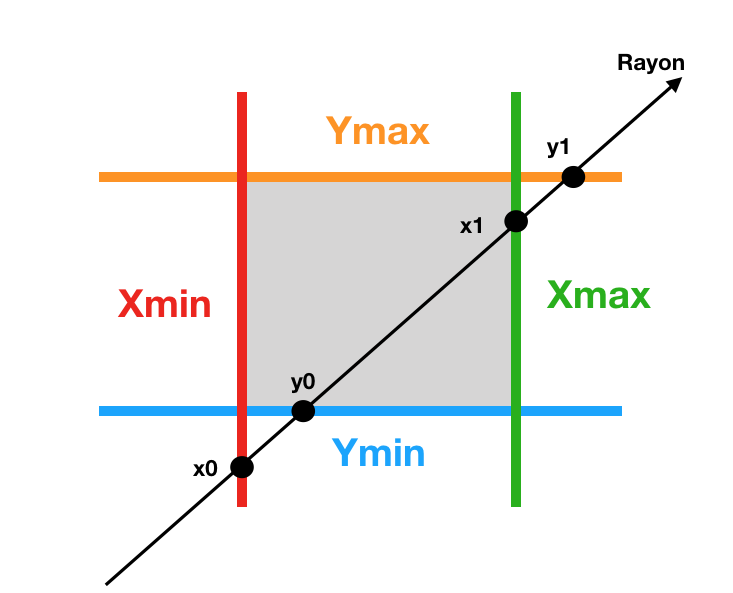
\includegraphics[width=\linewidth]{images/AABB}
		\caption{Vue 2D d'un rayon intersectant la boite}
		\label{AABB}
	\end{subfigureth}
	\qquad
	\begin{subfigureth}{0.45\textwidth}
		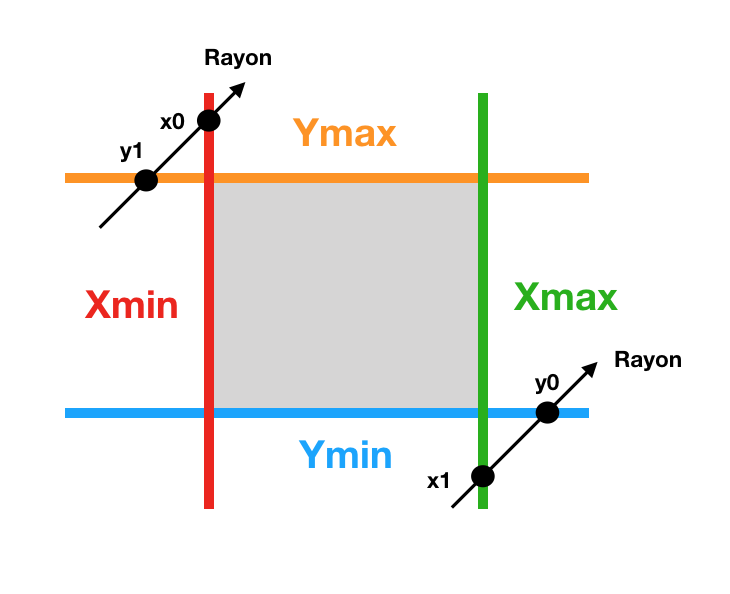
\includegraphics[width=\linewidth]{images/AABB2}
		\caption{Vue 2D de rayons n'intersectant pas la boite}
		\label{AABB2}
	\end{subfigureth}
	\caption{Illustrations de l'intersection Rayon/Boite en 2D}
\end{figureth}

Ainsi, on peut exprimer les points d'intersection entre le rayon et les plans délimitant la boite avec le système d'équations suivant :

\begin{align*}
X_{min} &= x_0 \times D_x + O_x 	& \Rightarrow 	& &	 x_0 = \frac{X_{min} - O_x}{D_x}, \\
X_{max} &= x_1 \times D_x + O_x 	& \Rightarrow 	& &	x_1 = \frac{X_{max} - O_x}{D_x}, \\
Y_{min} &= y_0 \times D_y + O_y 	& \Rightarrow	& &	y_0 = \frac{Y_{min} - O_y}{D_y}, \\
Y_{max} &= y_1 \times D_y + O_y 	& \Rightarrow	& &	y_1 = \frac{Y_{max} - O_y}{D_y}, \\
Z_{min} &= z_0 \times D_z + O_z	& \Rightarrow 	& &	z_0 = \frac{Z_{min} - O_z}{D_z}, \\
Z_{max} &= z_1 \times D_z + O_z 	& \Rightarrow 	& &	z_1 = \frac{Z_{max} - O_z}{D_z}. 
\end{align*}

On comprend d'après les figures \ref{AABB} et \ref{AABB2} que l'on va pouvoir déterminer si un rayon intersecte une boite en comparant les coordonnées des points d'intersection avec les plans. Notamment, si $x_0 > y_1$ ou $y_0 > x_1$ le rayon n'intersectera pas la boite (voir fig \ref{AABB2}). Dans le cas contraire, on appliquera le même principe sur $z$. Il n'y aura alors pas d'intersection si $max(x_0 ; y_0) > z_1$ ou $ z_0 > min(x_1 ; y_1)$. On notera que si le rayon est dirigé dans le sens inverse il faudra inverser les $\alpha_0$ et $\alpha_1$ ($\alpha$ correspondant aux coordonnées $x,y,z$) .

De cette façon on saura quelles sont les boites traversées par chaque rayons. Pour chaque feuille de l'\gls{octree}, c'est à dire les boites non-vides les plus basses dans l'arborescence, on testera les intersections entre les rayons et les faces situés dans la subdivision de l'espace correspondante uniquement. Ainsi, le calcul d'intersection ne se fait qu'entre peu de rayons et peu de faces.



\section{Analyse des résultats} \label{sect_resultatOctree}

Nous allons maintenant vérifier si l'implémentation de cette méthode permet d'accélérer le temps de calcul et sous quelles conditions. Comme évoqué précédemment, l'étape critique de l'algorithme est le test d'intersection rayons/éléments car la complexité initiale est quadratique et que ce processus se répète à chaque itérations jusqu'à atteindre \gls{RT60}. La complexité théorique en utilisant un \gls{octree} est de type $O(N\ln{M})$. 
Pour vérifier ce comportement nous rétitérons le même test qu'en introduction du chapitre \ref{sect_complexite} afin de comparer les résultats (voir tab. \ref{tabComplexite} et fig. \ref{complexite}). Ainsi, nous faisons varier le nombre $N$ de rayons et le nombre $M$ de triangles du maillage tels que $N = M$. À chaque mesure $N$ et $M$ sont multipliés par 2.

On constate dans un premier temps que le régime stationnaire commence plus tard en utilisant l'\gls{octree}. Effectivement, le temps d'une itération reste inférieur à $1s$ tant que $N$ est inférieur à 70~000 éléments contre 4~000 sans \gls{octree}. Ensuite on voit que la pente est quasiment linéaire ce qui coïncide à la complexité théorique établie dans la section \ref{sect_octree_gene} puisque en échelle logarithmique :
\begin {align*}
y = x\ln{x}  && \Rightarrow  && \ln{y} = \ln{x} + \ln{(\ln{x})} \approx \ln{x}.
\end{align*}
En observant le tableau \ref{tabComplexite}, on constate par exemple que pour $N = 262~144$ on divise par 1000 le temps de calcul par itération ce qui est très prometteur pour le calcul dans le théâtre d'Orange.

Dans un second temps nous ne faisons varier qu'un des deux paramètres et mesurons l'impact sur le temps de calcul (voir tab. \ref{tabComplexite1},  \ref{tabComplexite2} et fig. \ref{complexite1} et \ref{complexite2}). Sur ces figures on constate que le temps de calcul redevient quadratique lorsque le nombre de faces ou le nombre de rayons devient majoritaire sur l'autre paramètre. On constate par ailleurs qu'en fixant un nombre important de rayons le temps de calcul ne dépendra pas du nombre de faces du maillage. Cela est encourageant dans le cadre du théâtre d'Orange puisque des surfaces plus détaillées pourront être implementées sans grand impact sur le temps de calcul.

 \begin{figureth}
	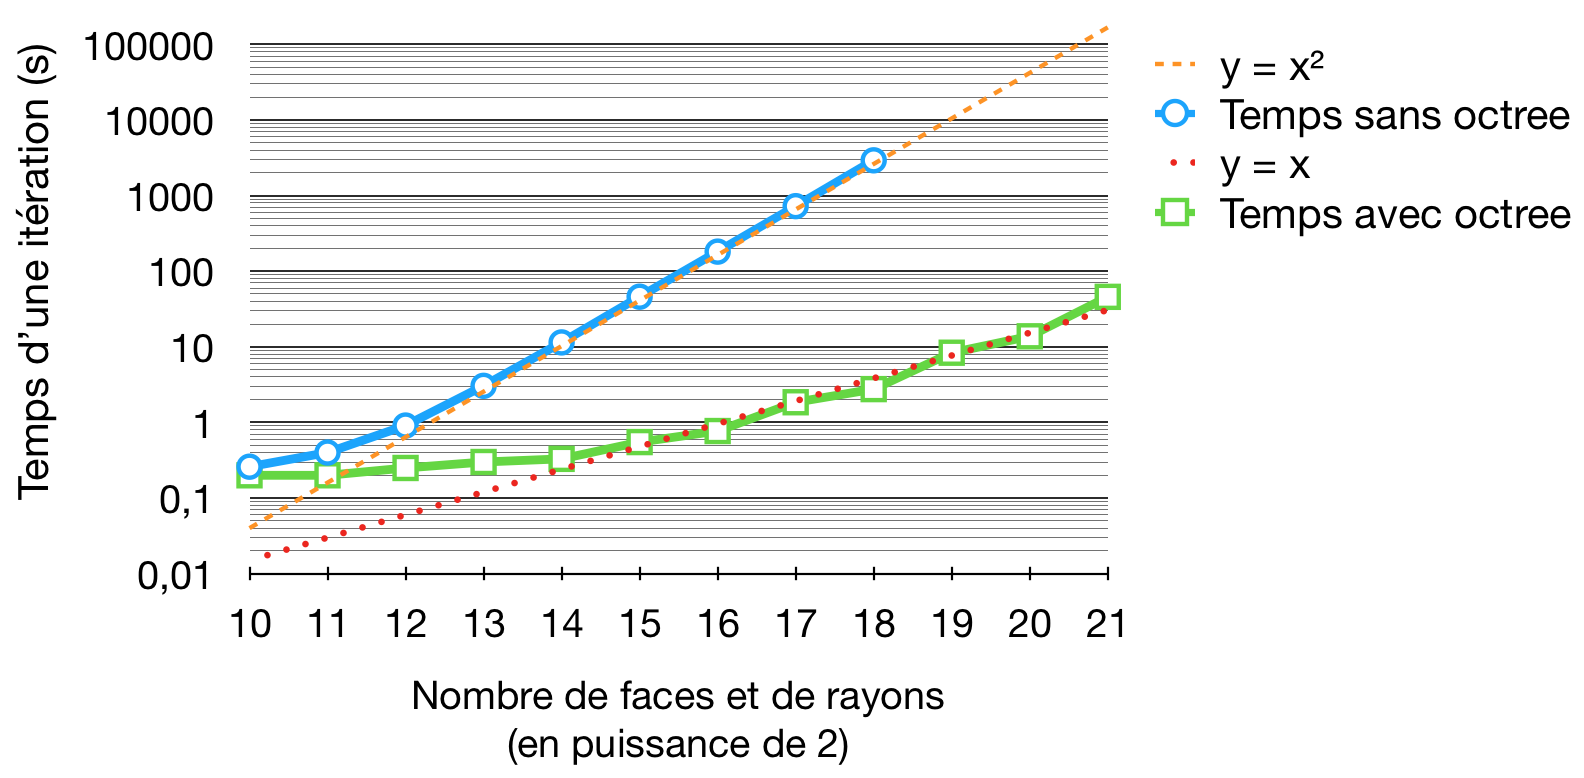
\includegraphics[width=\linewidth]{images/complexite}
	\caption{Temps de calcul (s) d'une itération en fonction du nombre de rayons et de faces avec N=M (échelle log)}
	\label{complexite}
\end{figureth}

\begin{tableth}
	\begin{tabular}{| c | c | c |}
		\hline
		Nombre de faces et de rayons & Temps \textbf{sans} \gls{octree} (s) & Temps \textbf{avec} \gls{octree} (s)\\
		  \hline
		  \hline
		   $2^{10}$ (=1~024) & 0,26 &	0,2 \\
		   \hline
		$2^{11}$ (=2~048)  & 0,4	& 0,2 \\
		   \hline
		$2^{12}$ (=4~096) & 0,91	& 0,25\\
		   \hline
		$2^{13}$ (=8~192) & 3,05 &	0,3\\
		   \hline
		$2^{14}$ (=16~384) & 11,44	&0,33\\
		   \hline
		$2^{15}$ (=32~768) & 46,02	&0,55 \\
		     \hline
		    $2^{16}$ (=65~536) & 181,61	& 0,77\\
		   \hline
		$2^{17}$ (=131~072) & 725,17	& 1,85\\
		\hline
		$2^{18}$ (=262~144) & 2927,9 & 2,76 \\
		\hline
		$2^{19}$ (=524~288) & X & 8,36 \\
		\hline
		$2^{20}$ (=1~048~576) & X & 13,78 \\
		\hline
		%$2^{21}$ (=2~097~152) & X & 45,83 \\
		%\hline
	 \end{tabular}
	\caption{Temps de calcul (s) d'une itération pour $N = M$}
	\label{tabComplexite}
\end{tableth}

%\begin{figureth}
%	\begin{subfigureth}{0.7\textwidth}
%		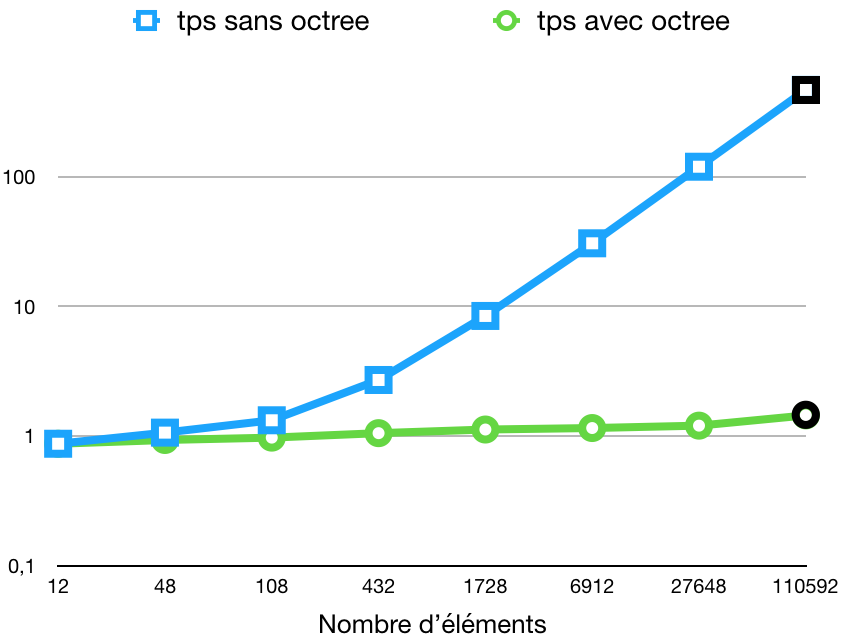
\includegraphics[width=\linewidth]{images/complexite1}
%		\caption{Temps (s) d'une itération en fonction du nombre d'éléments pour 100000 rayons (échelle log)}
%		\label{complexite1}
%	\end{subfigureth} \\
%\bigskip
%	\begin{subfigureth}{0.7\textwidth}
%		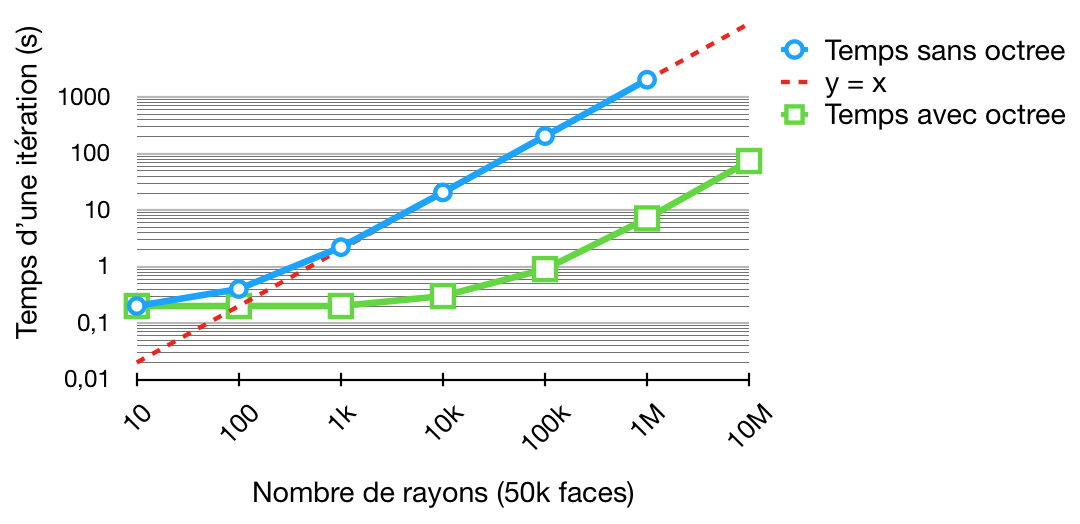
\includegraphics[width=\linewidth]{images/complexite2}
%		\caption{Temps (s) d'une itération en fonction du nombre de rayons pour 100000 éléments (échelle log)}
%		\label{complexite2}
%	\end{subfigureth}
%	\caption{Courbes de complexité}
%\end{figureth}

\clearpage

 \begin{figureth}
	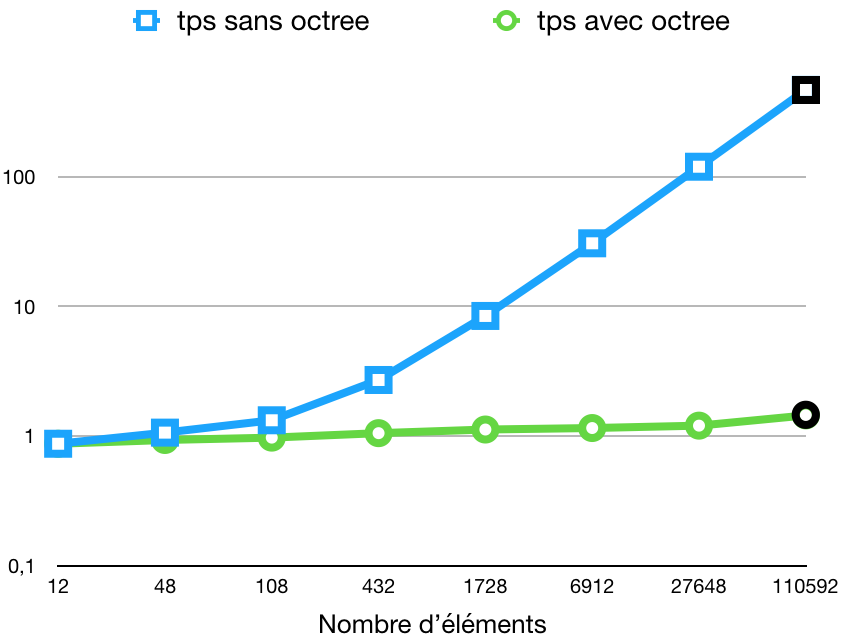
\includegraphics[width=\linewidth]{images/complexite1}
	\caption{Temps de calcul (s) d'une itération en fonction du nombre de faces pour 100k rayons (échelle log)}
	\label{complexite1}
\end{figureth}

\begin{tableth}
	\begin{tabular}{| c | c | c |}
			\hline
		Nombre de faces & Temps \textbf{sans} \gls{octree} (s) & Temps \textbf{avec} \gls{octree} (s)\\
		  \hline
		  \hline
		   12 &0,3&	0,3 \\
		   \hline
		48 &0,6	&0,4 \\
		   \hline
		192 & 1,2	&0,5\\
		   \hline
		768 & 3,55&	0,5\\
		   \hline
		3072 & 13,2	&0,6\\
		   \hline
		12288 &51	&0,7 \\
		     \hline
		     49152 & 203,6	&0,9\\
		   \hline
		196608 & 808,2	&1,1\\
		\hline
		786432 & X & 1,7 \\
		\hline
		3145728 & X & 6,1 \\
		\hline
	 \end{tabular}
	\caption{Temps de calcul (s) d'une itération pour 100k rayons}
	\label{tabComplexite1}
\end{tableth}

\clearpage

 \begin{figureth}
	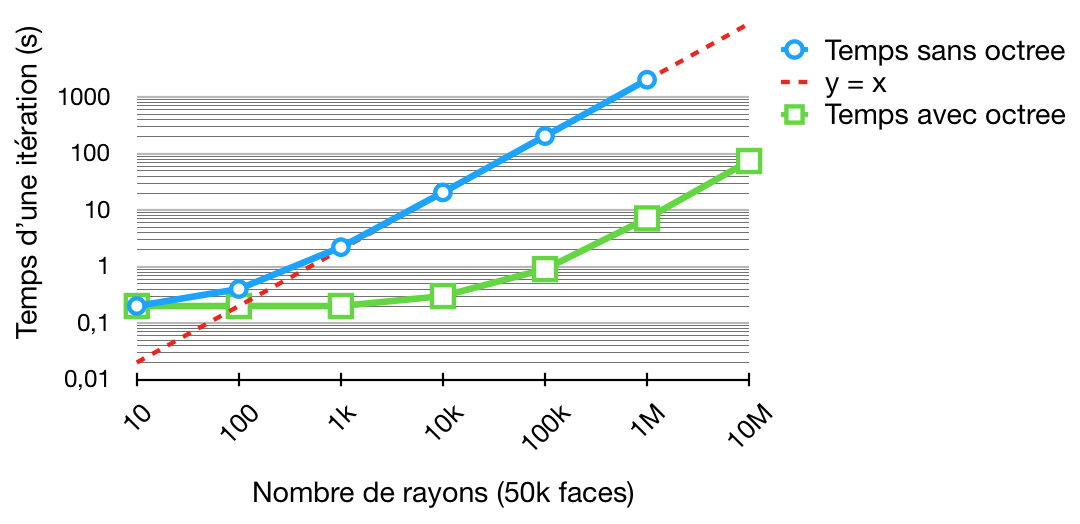
\includegraphics[width=\linewidth]{images/complexite2}
	\caption{Temps de calcul (s) d'une itération en fonction du nombre de rayons pour 50k faces (échelle log)}
	\label{complexite2}
\end{figureth}

\begin{tableth}
	\begin{tabular}{| c | c | c |}
		\hline
		Nombre de rayons & Temps \textbf{sans} \gls{octree} (s)& Temps \textbf{avec} \gls{octree} (s)\\
		  \hline
		  \hline
		   10 &0,2&	0,2 \\
		   \hline
		100 &0,4	&0,2 \\
		   \hline
		1k & 2,2	&0,2\\
		   \hline
		10k & 20,5&	0,3\\
		   \hline
		100k & 203,6&	0,9\\
		   \hline
		1M &2026 &	7,1 \\
		\hline
		10M & X &	73,7 \\
		\hline
	 \end{tabular}
	\caption{Temps de calcul (s) d'une itération pour 50k faces}
	\label{tabComplexite2}
\end{tableth}

%\begin{table}
%\footnotesize
%\center
%\begin{minipage}[t]{0.45\textwidth}
%	\begin{tabular}{|  m{2cm} |  m{2cm} |  m{2cm} |}
%		\hline
%		Nombre de faces & Temps \textbf{sans} \gls{octree} (s) & Temps \textbf{avec} \gls{octree} (s)\\
%		  \hline
%		  \hline
%		   12 &0,3&	0,3 \\
%		   \hline
%		48 &0,6	&0,4 \\
%		   \hline
%		192 & 1,2	&0,5\\
%		   \hline
%		768 & 3,55&	0,5\\
%		   \hline
%		3072 & 13,2	&0,6\\
%		   \hline
%		12288 &51	&0,7 \\
%		     \hline
%		     49152 & 203,6	&0,9\\
%		   \hline
%		196608 & 808,2	&1,1\\
%		\hline
%		786432 & X & 1,7 \\
%		\hline
%		3145728 & X & 6,1 \\
%		\hline
%	 \end{tabular}
%	\caption{Temps de calcul d'une itération pour 100k rayons}
%	\label{tabComplexite1}
%\end{minipage}
%\hfill
%\begin{minipage}[t]{0.45\textwidth}
%	\begin{tabular}{|  m{2cm} |  m{2cm} |  m{2cm} |}
%		\hline
%		Nombre de rayons & Temps \textbf{sans} \gls{octree} (s)& Temps \textbf{avec} \gls{octree} (s)\\
%		  \hline
%		  \hline
%		   10 &0,2&	0,2 \\
%		   \hline
%		100 &0,4	&0,2 \\
%		   \hline
%		1k & 2,2	&0,2\\
%		   \hline
%		10k & 20,5&	0,3\\
%		   \hline
%		100k & 203,6&	0,9\\
%		   \hline
%		1M &2026 &	7,1 \\
%		\hline
%		10M & X &	73,7 \\
%		\hline
%	 \end{tabular}
%	\caption{Temps de calcul d'une itération pour 50k faces}
%	\label{tabComplexite2}
%\end{minipage}
%\end{table}



% \begin{figureth}
%	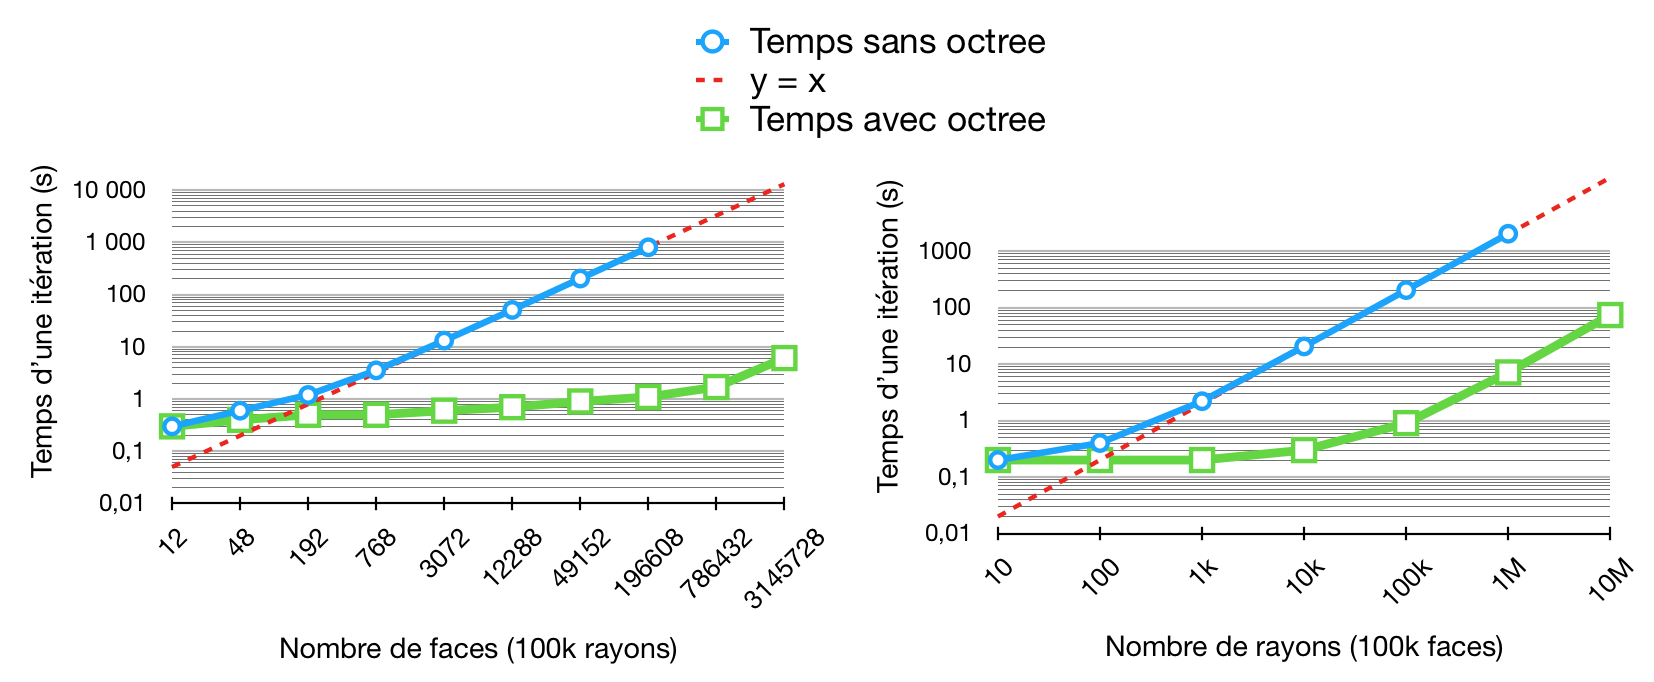
\includegraphics[width=\linewidth]{images/complexiteBis}
%	\caption{Courbes de complexité donnant le temps (s) avec et sans octree d'une itération en échelle logarithmique}
%	\label{complexiteBis}
%\end{figureth}






\chapter{Validation}
	\citationChap{
	L'observateur modifie ce qu'il observe. Certains événements ne se produisent que parce qu'ils sont observés. Sans personne pour les voir ils n'existeraient pas. 
	}{Bernard Werber}
	\minitoc
	\newpage
	
\section*{Introduction}

Dans le chapitre précédent, nous avons détaillé le fonctionnement de l'algorithme conçu pour analyser l'acoustique d'une salle. La méthode utilisée couple les principes de lancer de rayons, de sources-images et d'extrapolation stochastique. Elle vise à répondre aux problématiques de calcul acoustique en environnement complexe de manière géométrique et disrètisée. Géométrique, car seuls les effets de réflexion et absorption sont pris en compte et discrétisée car l'énergie d'onde n'est pas portée par une sphère mais par un grand nombre de rayons repartis de manière uniformes. Ainsi, il est essentiel de confirmer la justesse de ses approximations en les confrontant à des modèles théoriques. Dans ce chapitre, nous allons valider l'algorithme d'un point de vu physique et analyser ses performances. Nous allons donc choisir salles bien particulières afin d'effectuer cette validation de manière expérimentale. Tout d'abord nous vérifierons le bon comportement des rayons grâce à une analyse visuelle. Ensuite nous validerons la mesure d'un point de vu physique en comparant des réponses impulsionnelles obtenue avec des résultats théoriques.

\section{Analyse visuelle}
\subsection{Propagation de rayons}

Avant de tester la justesse des résultats d'un point de vu physique, il est bon d'en vérifier la justesse géométrique. Ainsi, nous analysons si les rayons ne traversent pas les parois et que la boite englobante assure bien son rôle. Pour cela, nous importons les rayons générés par notre logiciel dans des configurations de salles simples. En propageant les rayons dans un petit labyrinthe nous confirmons qu'ils s'arrêtent bien à la paroi la plus proche et qu'ils sont ainsi contenus à l'intérieur de la salle. 


\begin{figureth}
		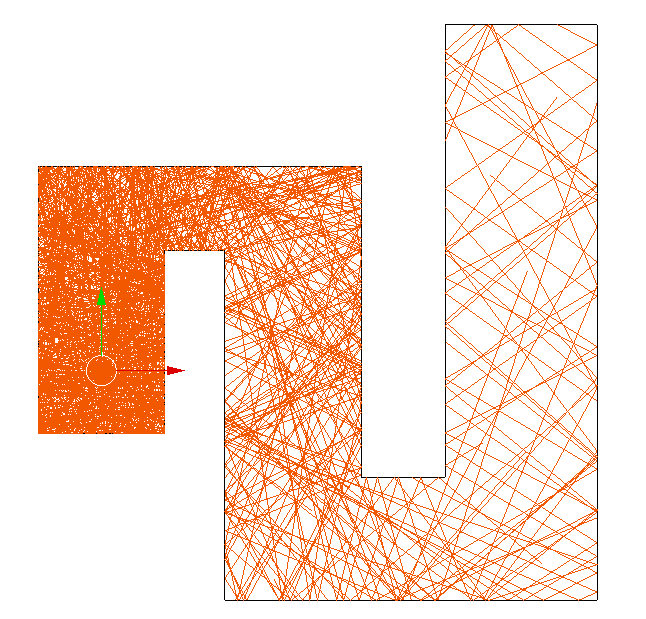
\includegraphics[width=0.5\linewidth]{images/test0}
		\caption{Propagation des rayons dans un labyrinthe}
		\label{test0}
\end{figureth}		

\subsection{Boite englobante}

De la même manière nous confirmons le bon fonctionnement de la boite englobante en utilisant une salle cubique dont on n'a gardé que les coins. On voit sur la figure \ref{testBE} que les rayons sont bien stoppés par une paroi invisible. Par ailleurs en effectuant une rotation de $45\degres$ sur chacun des axes on constate bien que la boite invisible englobe la salle.
\begin{figureth}		
	\begin{subfigureth}{0.45\textwidth}
		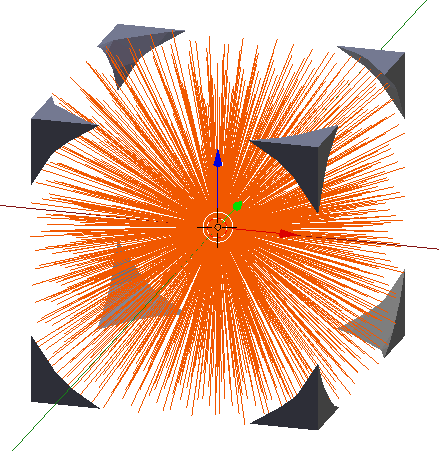
\includegraphics[width=\linewidth]{images/testBE}
		%\caption{Propagation des rayons dans un labyrinthe}
		%\label{testBE}
	\end{subfigureth}
	\quad
	\begin{subfigureth}{0.45\textwidth}
		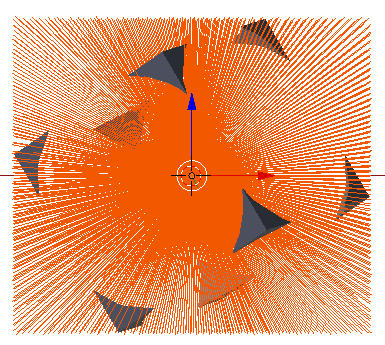
\includegraphics[width=\linewidth]{images/testBEbis}
		%\label{testBEbis}
	\end{subfigureth}
	\caption{Absorption des rayons par une boite englobante}
	\label{testBE}
\end{figureth}

\subsection{Rayons captés}
Nous vérifions finalement que les rayons captés par le récepteur sont bien portés par des cônes. Pour cela nous affichons sur blender uniquement les rayons générant une source image et les traçons depuis celle-ci.

\begin{figureth}
	\begin{subfigureth}{0.45\textwidth}
		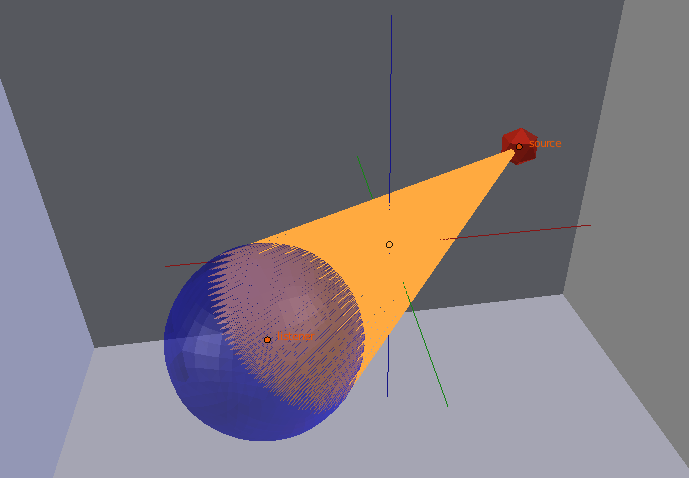
\includegraphics[width=\linewidth]{images/testBeam}
		\caption{Propagation des rayons depuis la source vers le récepteur.}
		\label{testBeam}
	\end{subfigureth}
	\quad
	\begin{subfigureth}{0.45\textwidth}
		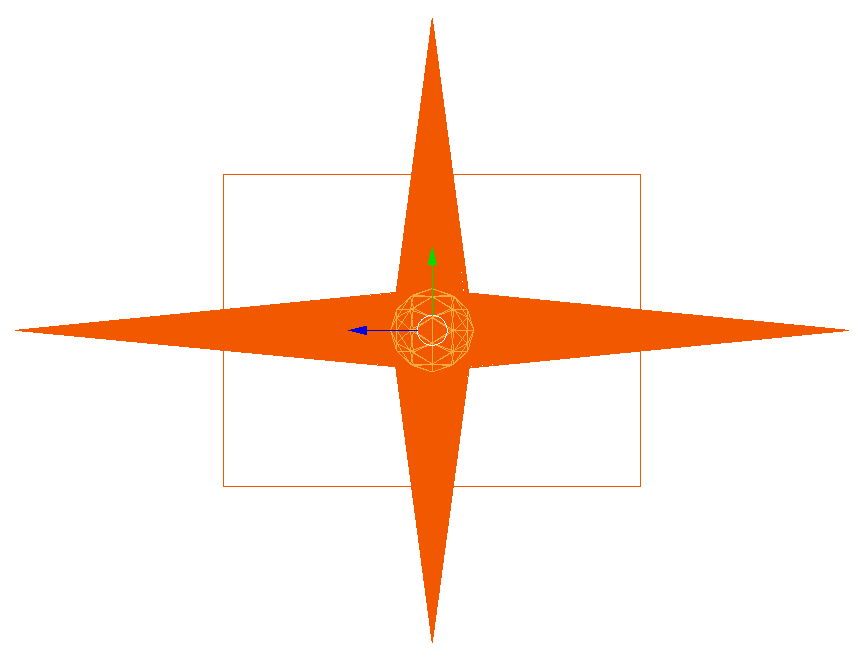
\includegraphics[width=\linewidth]{images/testBeam2}
		\caption{Propagation des rayons depuis les sources-images vers le récepteur à l'ordre 1.}
		\label{testBeam2}
	\end{subfigureth}
	\caption{Visualisation des rayons captés par le récepteur à l'ordre 0 et 1 récepteur (100000 rayons au total)}
\end{figureth}



%\section{Validation}

\section{Décroissance quadratique}


\begin{figureth}
	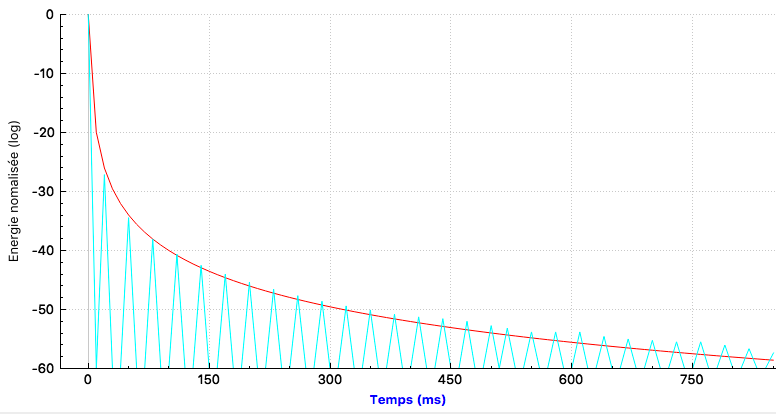
\includegraphics[width=0.8\linewidth]{images/test1}
	\caption{Réponse impulsionnelle en espace libre pour 3 millions de rayons (bleu) échantillonnée à 100Hz et fonction $f(x)=\frac{2}{x^2}$ (rouge)}
	\label{test1}
\end{figureth}


Suite à ces vérifications préliminaires, le premier test à réaliser pour analyser le comportement physique de l'algorithme est celui décrit dans la section \ref{sect_discretise}. Il s'agit de vérifier si l'utilisation d'un grand nombre de rayons et d'un récepteur de diamètre fixe permet de retrouver la loi de décroissance en $d^2$. Effectivement :
\begin{equation}
\frac{n}{N} = \frac{\int_s dS}{\int_{\sigma} dS} = \frac{\pi r^2}{4\pi d^2},
\end{equation}
avec :
\begin{itemize}
\item$n$ : le nombre de rayons captés,
\item$N$ : le nombre de rayons total,
\item$s$ : la surface (disque) constante du récepteur captant des rayons,
\item$\sigma$ : la surface de la sphère d'émission,
\item$r$ : le rayon constant du récépteur,
\item$d$ : le rayons de la sphère d'émission, autrement dit la distance entre le source-image et le récepteur.
\end{itemize}


Pour effectuer ce test, nous plaçons une source et un récepteur de rayons $1m$ au centre d'un cube de $10m$ de coté. Afin de simuler des mesures en espace libre (c'est à dire sans aucune paroi) où le récepteur s'éloigne de la source, nous allons affecter au cube des matériaux $100\%$ absorbants sur toutes ses parois sauf celles sur l'axe des $X$ qui seront $100\%$ réfléchissantes. Ainsi, cela revient à effectuer une mesure tous les $10m$, soit le temps d'aller retour des rayons du centre du cube jusqu'aux parois. N'ayant des réflexions que sur un axe, on reproduit une propagation en espace libre puisque seuls les rayons contenus dans le cône autour de l'axe $X$ conserveront leur énergie. Cependant, les rayons se réfléchissant en X et en -X de manière synchrone, on aura deux fois plus de rayons que si l'on se plaçait en espace libre. Nous pouvons comparer le résultat pour 30 itérations avec la fonction :

\begin{equation*}
f(x) = \frac{2}{x^2}.
\end{equation*}
Pour ce test, l'absorption de l'air a été désactivée afin de ne prendre en compte que la décroissance d'énergie portée par les rayons perçus. On observe bien sur la figure \ref{test1} que l'énergie suit la courbe de décroissance quadratique.
 		
		
\section{Cas de la salle sphérique}

Le deuxième test consiste à vérifier que l'énergie est bien conservée. Pour cela, nous plaçons une source et un récepteur de diamètre $1m$ au centre d'une sphère $100\%$ réfléchissante de diamètre $4m$. Ainsi à chaque itération, l'ensemble des $1000$ rayons revient se croiser au centre de la sphère et sont donc tous captés par le récepteur. Nous obtenons une réponse impulsionnelle de la forme d'une peigne de Dirac (voir fig. \ref{test2RIR}). L'écart entre chaque pic est de $11,76 ms$ ce qui correspond bien à une distance de $4m$ parcourue à la vitesse du son fixée à $340m/s$. Pour éviter la dispersion des rayons il est nécessaire d'avoir une sphère très bien raffinée. Celle utilisée pour le test possède $320000$ triangles. Notons que nous pouvons traiter rapidement ce nombre conséquent de triangles grâce à l'utilisation de l'\gls{octree}. Par ailleurs, la fréquence d'échantillonnage est descendue à 1000Hz pour s'assurer que les sources-images de chaque itération soient parfaitement synchronisées dans le calcul de l'énergie. On pourra par ailleurs importer les sources-images sous Blender et constater qu'elles sont bien réparties sur des sphères dont le diamètre augmente de $4m$ à chaque itération (voir fig. \ref{test2SI})

\begin{figureth}
	\begin{subfigureth}{0.45\textwidth}
		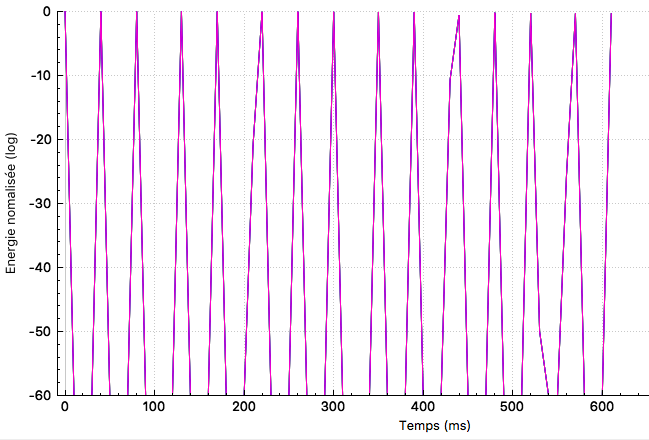
\includegraphics[width=\linewidth]{images/test2RIR}
		\caption{Réponse impulsionnelle dans une sphère 100\% réfléchissante pour 12 itérations}
		\label{test2RIR}
	\end{subfigureth}
	\quad
	\begin{subfigureth}{0.45\textwidth}
		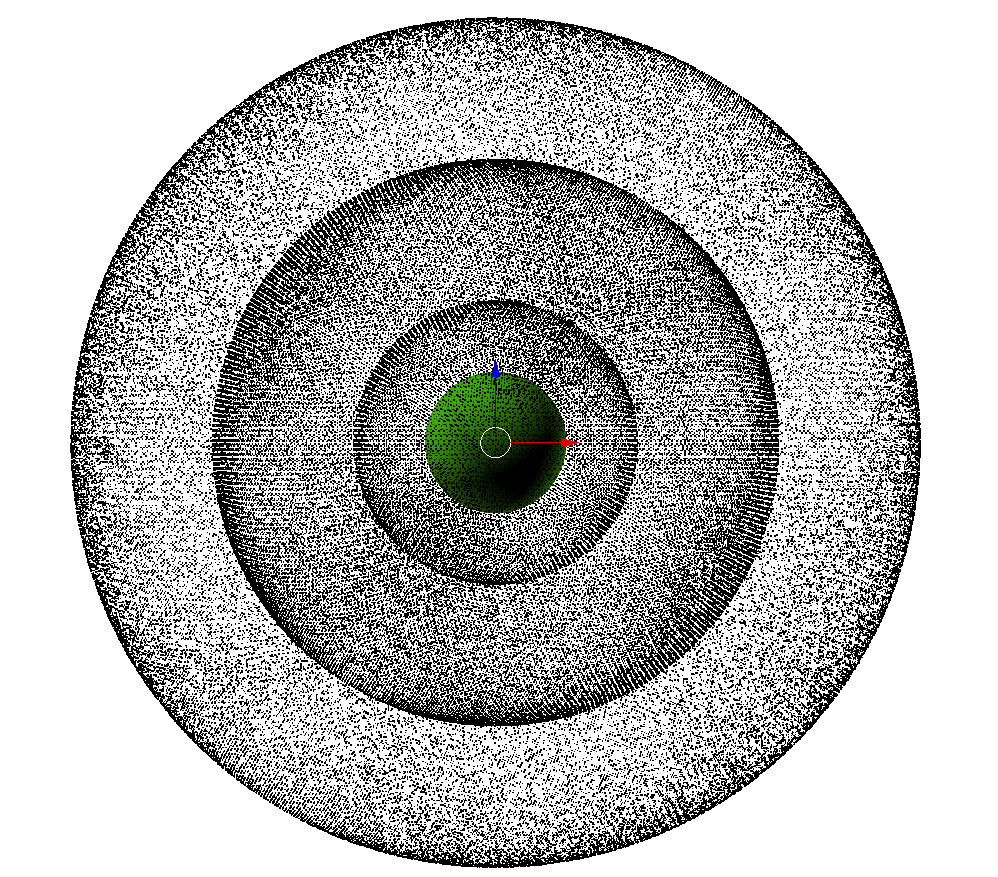
\includegraphics[width=\linewidth]{images/test2SI}
		\caption{Position des sources images dans le cas d'une sphère 100\% réfléchissante pour 4 itérations}
		\label{test2SI}
	\end{subfigureth}
	\caption{Cas d'une sphère 100\% réfléchissante}
\end{figureth}

Si l'on active l'absorption de l'air, on constate bien que les hautes fréquences sont plus absorbées que les basses fréquences en fonction de la distance (voir fig. \ref{test2absair}). Notamment au bout de 1700ms soit 578m, les fréquences à 8kHz ont quasiment totalement été absorbées par l'air, pour une température de 20°C et une pression relative de 50\%.

%On peut aussi vérifier ce comportement dans le cas plus général d'un ellipsoïde de révolution. Celui-ci peut être créé sous Blender à l'aide de l'add-on "\textit{Extra Objects}" en configurant un objet de type "\textit{XYZ Math Surface}". Nous créons alors un ellipsoïde avec les équations suivantes :

\begin{figureth}
	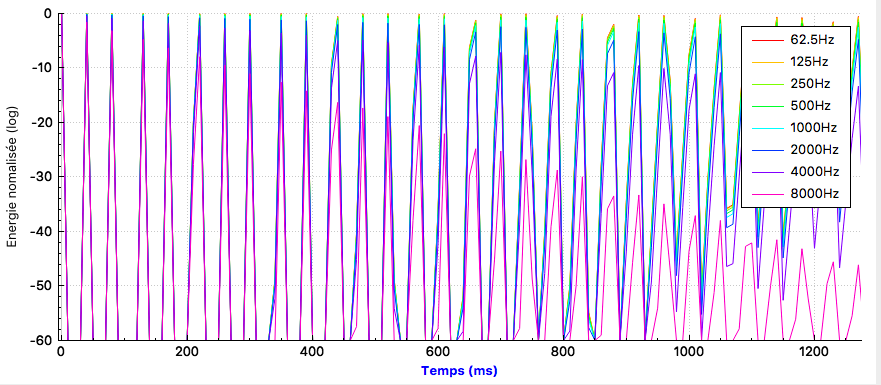
\includegraphics[width=\linewidth]{images/test2absair}
	\caption{Réponse impulsionnelle dans une sphère de $20m$ de diamètre, 100\% réfléchissante, pour 30 itérations avec absorption de l'air}
	\label{test2absair}
\end{figureth}



\section{Cas de la salle cubique}

Le dernier test consiste à comparer les résultats de calcul avec une formule analytique pour une pièce de type pavé droit. La formule \cite[p. 182-189]{mcgovern} est la suivante : 

%\begin{align}
%A &=  (-1)^i \\
%B &= i + 0,5 - 0,5 \times (-1)^i \\
%P_{si} &= A \times P_s + B \times D
%\end{align}
%
%Que l'on peut plus simplement écrire :

\begin{align}
P_{si} = i \times D + P_s \times (-1)^i,
\end{align}
avec : 
\begin{itemize}
\item$i \in (-n, n)$ et $n \in \mathbb{N}$,
\item$P_{si}$ : La coordonnée de la position de la source image selon X, Y ou Z,
\item$P_s$ : La coordonnée de la position de la source selon X, Y ou Z,
\item$D$ : La dimension de la salle selon X, Y ou Z.
\end{itemize}

\begin{figureth}
		\includegraphics[width=\linewidth]{images/test3_0}
		\caption{Position des sources-images pour une salle cubique, 10 itérations}
		\label{test3}
	\end{figureth}

On constate alors qu'on a une superposition parfaite des sources-images dans l'espace (voir fig. \ref{test3}) puisque l'écart des positions des sources-images expérimentales obtenues par lancer de rayons et les sources-images théoriques obtenues par formule analytique est inférieur à la précision machine (soit $10^{-6}$m pour des float). On mesure également l'erreur relative des énergies source-image par source-image en prenant comme valeur théorique $\frac{1}{d^2}$ où $d$ est la distance de la source-image au récepteur. On a alors :
\begin{align}
\epsilon_{rel} = \frac{|E_{exp}-E_{theo}|}{E_{theo}}.
\end{align}

On note que la salle est un pavé dont les dimensions sont respectivement 2m, 3m et 4m sur les axes X, Y, Z. d'arrête, que le récepteur a un diamètre de 40cm et qu'il n'est pas superposé à la source. On peut observer que l'erreur moyenne est inférieure à 1\% avec des pics pouvant aller jusqu'à 3\%. Par ailleurs étant donné que plus les sources-images sont éloignées moins leur énergie sera importante, autrement dit elles seront moins entendues par l'auditeur, on peut résonner avec la norme infinie telle que :
\begin{align}
\epsilon_{\infty} = \frac{|E_{exp}-E_{theo}|}{\max(E_{theo})}.
\end{align}

On constate alors une erreur relative inférieure à 0,5\% pour 1~000~000 de rayons (voir fig. \ref{test3_2}). On voit également qu'en augmentant le nombre de rayons on améliore la précision des 150 premières sources-images et les 1300 sources-images suivantes reste bien dans une plage d'erreur inférieures à 5\% (voir fig. \ref{test3_3}) et 0,2\% en norme infinie (voir fig. \ref{test3_4}).

\begin{figureth}
	\begin{subfigureth}{0.8\textwidth}
		\includegraphics[width=\linewidth]{images/test3_1}
		\caption{Erreur relative pour 1~000~000 rayons}
		\label{test3_1}
	\end{subfigureth}
	\begin{subfigureth}{0.8\textwidth}
		\includegraphics[width=\linewidth]{images/test3_2}
		\caption{Erreur relative pour 4~000~000 rayons}
		\label{test3_2}
	\end{subfigureth}
	\begin{subfigureth}{0.8\textwidth}
		\includegraphics[width=\linewidth]{images/test3_3}
		\caption{Erreur relative en norme infinie pour 1~000~000 rayons}
		\label{test3_3}
	\end{subfigureth}
	\begin{subfigureth}{0.8\textwidth}
		\includegraphics[width=\linewidth]{images/test3_4}
		\caption{Erreur relative en norme infinie pour 4~000~000 rayons}
		\label{test3_4}
	\end{subfigureth}
	\caption{Erreur relative des énergies des sources-images dans une salle parallélépipédique}
\end{figureth}
		
Dans un second temps, on assigne à chacune des six faces de la salle parallélépipédique des coefficients d'absorption différents. On met à jour les énergies des sources-images théoriques par la formule suivante :
\begin{align}
E_{si} = \frac{1}{d} \times \prod_{j=0}^{6}{(1-a_j^{\alpha_j})}, 
\end{align}
avec : 
\begin{itemize}
\item $a_j$ : les coefficient d'absorption de la j-ème paroi,
\item $\alpha_j  = 0,5i - 0,25b + 0,25b(-1)^i$,
\item $ i \in (-n, n), n \in \mathbb{N}$,
\item  $
 \left \{
   \begin{array}{r c c c l}
       b & = & 1 & si & X_j \geqslant 0, \\
       b & = & -1 & si & X_j < 0,
   \end{array}
   \right.$
\item $X_j$ : les coordonnées selon [x, -x, y, -y, z, -z].
\end{itemize}

\begin{figureth}
	\begin{subfigureth}{0.8\textwidth}
		\includegraphics[width=\linewidth]{images/test3_5}
		\caption{Erreur relative}
		\label{test3_5}
	\end{subfigureth}
	\begin{subfigureth}{0.8\textwidth}
		\includegraphics[width=\linewidth]{images/test3_6}
		\caption{Erreur relative en norme infinie}
		\label{test3_6}
	\end{subfigureth}
	\caption{Erreur relative des énergies des sources-images dans une salle parallélépipédique avec absorption des parois pour 4~000~000 rayons}
\end{figureth}


On constate que l'erreur relative source-image par source-image ainsi que l'erreur en norme infinie restent bien inférieures aux valeurs indiquées précédemment (voir fig. \ref{test3_5} et \ref{test3_6}). De la même manière, on implemente l'absorption atmosphérique dans le calcul de l'énergie théorique telle que :
\begin{align}
E_{si} = \frac{1}{d} \times \prod_{j=0}^{6}{(1-a_j^{\alpha_j})} \times e^{-m.d}, 
\end{align}
avec $m$ le coefficient d'absorption décrit dans la section \ref{sect_absAIr}. La température est fixée à $20°C$ et l'humidité relative à $30\%$. On obtient encore une fois pour un million de rayons des erreurs relatives sur l'énergie inférieures à 5\% (voir fig. \ref{test3_8}) et à 0,2\% en norme infinie (voir fig. \ref{test3_9}).


\begin{figureth}
	\begin{subfigureth}{0.8\textwidth}
		\includegraphics[width=\linewidth]{images/test3_8}
		\caption{Erreur relative avec absorption de l'air}
		\label{test3_8}
	\end{subfigureth}
	\begin{subfigureth}{0.8\textwidth}
		\includegraphics[width=\linewidth]{images/test3_9}
		\caption{Erreur relative en norme infinie}
		\label{test3_9}
	\end{subfigureth}
	\caption{Erreur relative des énergies des sources-images dans une salle parallélépipédique avec absorption de l'air pour 1~000~000 rayons}
\end{figureth}

\chapter{Outil logiciel}
	\citationChap{
	L'éducation est le logiciel de l'ordinateur central qui programme l'avenir des sociétés.
	}{Joseph ki zerbo}
	\minitoc
	\newpage
	
La figure \ref{synopsis} présente de manière synthétique l'architecture logicielle développée au cours du projet. 
%
\begin{figureth}
	\includegraphics[width=0.9\linewidth]{images/synopsis}
	\caption{Synopsis de l'architecture logiciel développé pour le calcul d'acoustique de salle}
	\label{synopsis}
\end{figureth}

	
\section{Utilisation générique du logiciel}
	
La force de ce développement logiciel est que l'utilisateur n'a pas besoin d'effectuer de manipulations complexes pour obtenir les résultats de calcul d'acoustique de salle. Il pourra travailler directement sur son maillage dans le logiciel \gls{cao} et lancer le calcul. Blender permet de développer des scripts en Python qui peuvent par la suite être installés sous forme de \textit{add-on}. L'interface homme-machine de Blender est donc complètement modulable et personnalisable. Un \textit{add-on} a donc été développé dans le cadre de ce projet et son rôle est de fournir un maillage adapté à un outil de calcul externe puis de réimporter les résultats dans Blender pour pouvoir les visualiser (voir fig. \ref{logiciel}). Le coeur du calcul s'effectue sur un programme séparé développé en C++ (via Qt creator). L'utilisation d'un langage compilé permet d'optimiser le temps de calcul et le fait d'être un programme séparé permet aux utilisateurs réticent à utiliser Blender pour pouvoir tout de même s'en servir. Il suffit de placer un fichier de maillage au format \gls{obj} dans le répertoire adéquate pour pouvoir lancer le calcul. A noter que le format \gls{obj} permet d'obtenir les informations sur les vertices, les normales et les faces ainsi que les matériaux. D'autres formats de maillages pourront être implémentés dans un développement futur.

\begin{figureth}
	\includegraphics[width=0.7\linewidth]{images/logiciel}
	\caption{Communication entre l'add-on Blender et l'outil de calcul}
	\label{logiciel}
\end{figureth}


Le add-on développé dans la cadre de ce projet possède quelques boutons (voir fig \ref{add-on}). La première étape consiste à notifier le répertoire de donnée de l'outil de calcul afin de pouvoir exporter le fichier de maillage. En utilisant le bouton "Run", Blender transforme les faces des objets sélectionnés en triangles et les exporte au format \gls{obj}. Dans le fichier de maillage, chaque objet est différencié par un en-tête comprenant son nom. S'en suit les coordonnées de l'ensemble de ses sommets (ou vertices), de ses textures et de ses normales. Ensuite sont regroupées par matériaux, les faces par combinaison de trois vertices, d'une texture et d'une normale. Un vecteur de sommets et un vecteur de normales sont remplis face par face en conservant le même ordre. Ces deux vecteurs stockent ainsi la totalité du maillage. Les textures quant à elles ne nous sont pas utiles. Les coefficients d'absorption des matériaux sont aussi assemblés dans un vecteur en les classant face par face en respectant l'ordre établi précédemment. Par défaut, une source et un récepteur sont positionnés au point [0, 0, 0]. Le rayon de mesure du récepteur est de 1m. Cependant, l'utilisateur pourra changer ces paramètres en créant des objets source et récepteur dans Blender. Pour être reconnus et discriminés du maillage, ces objets doivent respectivement comporter les mots "\textit{source}" et "\textit{listener}" dans leur nom. L'algorithme déterminera alors le centre des objets sources et des récepteurs en calculant la moyenne des coordonnées des sommets. Le rayon de mesure du récepteur correspond au rayon de la sphère circonscrite à l'objet "\textit{listener}". Notons qu'il est possible de placer plusieurs sources. L'ensemble des calculs se réaliseront séquentiellement pour une source après l'autre. Un seul récepteur est pris en compte. L'add-on Blender permet de mettre à jour uniquement les informations sur les sources et récepteurs sans avoir besoin de recharger tout le maillage. 
\begin{figureth}
	\includegraphics[width=\linewidth]{images/add-on}
	\caption{Add-on Blender et assignation des matériaux}
	\label{add-on}
\end{figureth}
Par ailleurs l'utilisateur assignera aux différentes parois un type de matériau en faisant apparaitre dans son nom la référence du matériau issue de la base de donnée Odéon (voir section \ref{sect_lectMat}). De nombreux autres paramètres sont configurables grâce à une \gls{ihm} générée par Qt (voir fig. \ref{ihm}). On peut alors paramètrer la température, la pression relative, le nombre de rayons, etc. L'outil permet donc d'afficher la \gls{rir} et d'écouter un fichier audio révérberé grace au calcul effectué. Il est ensuite possible de visualiser certains résultats directement sur Blender comme les rayons ou les sources-images par exemple (voir fig \ref{import}). Un option permet aussi de projeter les sources-images sur les parois de la salle afin de visualiser de manière plus intuitive d'où proviennent les reflexions (voir fig \ref{projete}).
\begin{figureth}
	\includegraphics[width=\linewidth]{images/import}
	\caption{Affichage des rayons (une itération) et des sources-images (-60dB) dans le théâtre d'Orange}
	\label{import}
\end{figureth}


\begin{figureth}
	\includegraphics[width=0.8\linewidth]{images/projete}
	\caption{Projeté des sources-images sur les parois du théâtre d'Orange}
	\label{projete}
\end{figureth}


\section{Paramètres de sortie}
L'étude de l'acoustique d'un bâtiment passe par le calcul de différents paramètres obtenus à partir de la \gls{rir}. Ceux-ci permettent de qualifier les qualités d'une salle. C'est Leo L. Beranek qui proposa le premier, bien après les études de Sabine, une approche de définition générale de la qualité acoustique d'une salle de spectacle. Il propose de comparer différentes salles de concert par des experts (chefs d’orchestre, interprètes et critiques musicaux). Ceux-ci ont permis de dégager sept facteurs perceptifs :
\begin{itemize}
	\item Reverberance : réverbérance, évaluation subjective du phénomène de réverbération ;
	\item Loudness : puissance sonore ;
	\item Spaciousness : spaciosité, sensation d'espace et d'enveloppement sonore ;
	\item Clarity : clarté ou transparence ;
	\item Intimacy : intimité, sensation de proximité sonore ;
	\item Warmth : chaleur apportée par la coloration des timbres par la salle ;
	\item Hearing on stage : aptitude pour les musiciens, les comédiens ou les conférenciers (donc dans le contexte d'une salle de spectacle uniquement) à s'entendre correctement. 
\end{itemize}

Dans notre étude nous nous appuierons sur certains de ces paramètres et calculerons ceux qui sont le plus couramment utilisés. Nous utilisions pout cela les formules implémentées dans le logiciel Odéon \cite[p.87-92]{odeonManuel}. %Les autres, moins pertinent pourront être implémentés à posteriori. Par exemple la spaciosité est pertinente dans les environnements où l'auditeur est proche de la source et où la source est volumineuse.
\subsection{Réverbérance : $T_{30}$}
Nous disposons de la réponse impulsionnelle de la salle et pouvons par consequent mesurer différent temps de réverbération. Un facteur qui est souvent utilisé dans les études acoustiques de bâtiments est le \gls{T30}. Celui-ci correspond au temps que l'énergie met pour passer de -5 à -35dB.

\subsection{Early Decay Time : EDT}
Il sera interessant de séparer les premières réflexions du champs diffus. Ce paramètre se nomme \gls{EDT} et correspond au temps pour que l'énergie diminue de 10dB.

\subsection{Clarté : $C_{80}$}
La clarté est un paramètre qui vise à exprimer la compréhensibilité exprimé en dB tel que :
%
\begin{equation}
C_{80} = 10\log{\left( \frac{E_{0\to80}}{E_{80\to\infty}} \right)},
\end{equation}
%
et $E_{a\to b}$ est la fraction d'énergie sonore comprise dans l'intervalle [a,b] telle que :
%
\begin{equation}
E_{a\to b} = \int_a^b p^2(t) dt. \footnotemark
\end{equation}
\citefnt[eq 74, p. 221]{jouhaneau}
Nous utilisons comme limite utile pour la compréhension de la parole la valeur de 80ms car c'est celle qui est le plus largement utilisée (introduite par Reichardt \cite[p.126]{Reichardt} en 1975). Précisons par ailleurs que ce facteur est subjectif, c'est à dire qu'il sera sensible à l'interpretation de l'auditeur en terme de psychoacoustique. Aussi, selon la répartition des premières réflexions, deux \gls{rir} dont la clarté calculée est identique pourra donner une clarté perçue différente \cite[p. 226]{jouhaneau}. %Il est d'usage de définir optimale entre -6 et 6 dB. Si la valeur est supérieure à cet intervalle, la salle répondra de manière sèche, et si elle est inférieure, le son direct sera noyé parmi les sons réverbérés et la salle sera dite « confuse » .
	
\subsection{Définition : $D_{50}$}
Le paramètre de \gls{D50} exprime en pourcentage le ratio entre les premières réflexions et le son réverbéré total. Il se calcul par la formule suivante :
\begin{equation}
D_{50} = \frac{E_{0\to50}}{E_{0\to\infty}}.
\end{equation}


\subsection{Temps central : $T_s$}
Le paramètre de \gls{D50} exprime le temps moyen de la répartition d'énergie :
\begin{equation}
T_s =  \frac{\sum\limits_{0}^{\infty} tE_t}{E_{0\to\infty}}.
\end{equation}

\subsection{Puissance sonore : SPL}
Le niveau de pression acoustique en dB ou \gls{spl} est défini tel que :
\begin{equation}
SPL =  10\log{E_{0\to\infty}}.
\end{equation}
Il est équivalent au terme G (gain par rapport au niveau produit par une source omnidirectionnelle placée à 10m en espace libre \footnote{ISO 3382-1, 2009}.

\subsection{Spaciosité : $LF_{80}$}
Pour déterminer la spaciosité, c'est à dire la largeur apparente de la source et l'enveloppement des auditeurs, on étudie le rapport entre les réflexions latérales et l'ensemble des réflexions précoces. Ce paramètre se calcul avec la formule suivante :
\begin{equation}
LF_{80} =   \frac{\sum\limits_{t=5}^{80} E_t \cos^2(\beta_t)}{E_{0\to80}}. 
\end{equation}


%\subsection{Speech Transmission Index : STI}
%Le \gls{STI} est un indice très interessant notamment pour l'étude de bâtiment où l'on transmet vocalement du texte.
	
\chapter*{Conclusion}
\addcontentsline{toc}{chapter}{Conclusion}

Dans cette partie, nous avons présenté les problématiques soulevées par une étude acoustique d'un monument antique. La géométrie complexe de ce type de bâtiment et leur taille colossale impose l'utilisation de méthodes de calcul approchées. Ainsi, par simulation des réflexions et absorptions des parois, il est possible d'étudier la réverbération d'une salle. Malgré les approximations inéluctables du modèle, nous avons prouvé que les lois de la physique sont respectées. Un algorithme rapide a été mis en place pour permettre aux utilisateurs de tester facilement et rapidement leurs hypothèses architecturales. Ainsi, le temps de calcul devient peu sensible aux nombres d'éléments du maillage ce qui est souvent limitant dans ce genre d'étude. Le fonctionnement de l'algorithme développé a été présenté en détail de même que les différents outils d'analyse qui en découlent. Celui-ci permet l'étude du graphe temporel de réverbération du bâtiment ainsi que la position dans l'espace des différentes réflexions sonores (voir fig \ref{projete}). Ces résultats pourront aussi être analysés à l'oreille en écoutant le son réverbéré émis depuis une ou plusieurs sources et entendu par un auditeur virtuel placé dans le bâtiment. %
%
%\begin{figureth}
%	\includegraphics[width=0.9\linewidth]{images/orange}
%	\caption{Représentation des réflexions des rayons sonores par projection des sources-images dans le théâtre d'Orange}
%	\label{orange}
%\end{figureth}
%

%Cet outil de calcul acoustique s'interface au logiciel Blender dans la continuité de l'étude présentée dans la partie \ref{part_1} de ce document.

Il y a cependant de nombreuses possibilités d'améliorations qui restent à l'étude pour ce type d'outil logiciel. Premièrement, l'écoute du signal sonore pourrait être rendue en trois dimensions grâce à des filtres binauraux. Ceux-ci permettent par l'intermédiaire d'un casque audio de transmettre un signal différent à chacune des deux oreilles afin de donner l'illusion d'espace et de profondeur. Cela est réalisable grâce au calcul de positionnement des sources-images dans l'espace. Tout en restant en position statique, l'auditeur pourra donc orienter son regard selon différentes directions et écouter en temps réel le son changer. Le contrôle de la direction pourrait alors être effectué au clavier ou à l'aide d'un casque avec "\textit{Head Tracker"}. En se plaçant en vu subjective dans le modèle 3D de Blender, on peut faire un premier pas vers l'analyse audiovisuelle immersive. Dans un second temps, dans un contexte ou la réalité virtuelle prend de plus en plus d'importance dans les applications d'aujourd'hui, on pourrait envisager de déplacer l'auditeur en temps réel et permettre ainsi une visite virtuelle complète du bâtiment.

Du point de vu des résultats d'analyse, il y a de nombreuses améliorations envisageables au niveau graphique. Cela pose certaines questions. Comment visualiser des résultats de calculs acoustiques ? Quelles sont les informations indispensables à recueillir pour un archéologue voulant étudier l'acoustique d'un monument ? 

De la même manière, est-il essentiel d'ajouter les effets de diffraction au modèle ? Si oui, quelle est la meilleur méthode ? Pourrait-on traiter de manière locale certains comportements acoustiques et les insérer ensuite dans le modèle par lancer de rayons ? Typiquement, pourrait-on analyser par méthode de résolution exacte (voir section \ref{sect_resExacte}) le comportement acoustique d'une colonne, ou de tout autre ornement avec un fort niveau de détail, puis de l'incorporer de manière analytique dans l'outil de lancer de rayons ? Ou bien, peut-on résonner avec des résolutions exactes pour les faibles fréquences et conserver notre approche par méthode couplées pour les hautes fréquences ?

Pour finir, nous l'avons déjà évoqué dans la section \ref{sect_rayon}, mais il serait également interessant d'utiliser des sources dont la directivité n'est pas uniforme. Cela serait d'ailleurs plus représentatif des cas réels et notamment de l'usage fait à Orange à l'origine du théâtre. Les sons étaient alors émis par des instruments de musique ou par la voix humaine éventuellement amplifiée par un masque.

 La prochaine partie vise à présenter concrètement comment s'utilise cet outil dans son état actuel autour du cas d'étude du théâtre antique d'Orange. Ainsi, nous tenterons d'analyser des hypothèses archéologiques précises grâce à l'étude acoustique du bâtiment.

%Ce sont des questions que nous allons pouvoir approfondir dans le partie suivante.



\newpage
	
% Biblio
 \bibliographystyle{francaissc}
 \bibliography{Part2/Biblio}
\addcontentsline{toc}{chapter}{Références}
